%% ============================================================================
%% AeroTray -- HardwareX manuscript, final English version
%% (MT5001 Mechatronic Systems Design, UTEC, 2026-2)
%% Compile with pdfLaTeX + BibTeX (Overleaf default). Each section lives in
%% sections/*.tex. Search for "TODO" and \tocheck{...} before submission.
%% ============================================================================
\documentclass[preprint,12pt,a4paper]{elsarticle}
%% ======================================================================
%% preamble.tex -- paquetes y macros comunes a todas las secciones
%% ======================================================================
\usepackage{iftex}
\ifXeTeX
  \usepackage{fontspec}
\else
  \usepackage[T1]{fontenc}
  \usepackage[utf8]{inputenc}
  \usepackage{lmodern}
  \usepackage{textcomp}
\fi
%% English typography with standard decimal point.
\usepackage[english]{babel}
\usepackage{amsmath,amssymb,bm}
\usepackage{graphicx}
\usepackage{booktabs,tabularx,multirow,longtable,array}
\usepackage{siunitx}
\usepackage{xcolor}
%% Shared palette with figuras_matlab_en/estilo_paper.m (adapted Okabe-Ito)
\definecolor{pAzul}{HTML}{0072B2}
\definecolor{pRojo}{HTML}{D55E00}
\definecolor{pVerde}{HTML}{009E73}
\definecolor{pOcre}{HTML}{B07A00}
\definecolor{pMorado}{HTML}{A0529A}
\definecolor{pGris}{HTML}{6E6E6E}
\usepackage{tikz}
\usetikzlibrary{arrows.meta,positioning,shapes.geometric,fit,calc,backgrounds}
\usepackage{subcaption}
\usepackage[section]{placeins}
\usepackage{enumitem}
\usepackage[colorlinks=true,linkcolor=blue!50!black,citecolor=blue!50!black,urlcolor=blue!60!black]{hyperref}
\makeatletter\g@addto@macro{\UrlBreaks}{\do\_\do\-\do\.}\makeatother

\sisetup{detect-all, range-phrase = \text{--}, per-mode = symbol, output-decimal-marker = {.},
         list-pair-separator = {\text{ and }}, list-final-separator = {\text{ and }}}
\setlist{itemsep=1pt,topsep=3pt}
\setlength{\emergencystretch}{3em}
\renewcommand{\arraystretch}{1.15}

%% ---------------------------------------------------------------- macros
\newcommand{\fn}[1]{\path{#1}}
\newcommand{\repourl}{\url{https://github.com/geo105/AeroTray}}
\newcommand{\us}{\,\si{\micro\second}}
\newcommand{\Rot}{\mathbf{R}}
\newcommand{\vect}[1]{\bm{#1}}
\newcommand{\ez}{\vect{e}_z}
\newcommand{\skw}[1]{[#1]_\times}
\newcommand{\T}{^{\!\top}}
\newcommand{\dd}{\mathrm{d}}
\newcommand{\sat}{\operatorname{sat}}
\newcommand{\diag}{\operatorname{diag}}
%% editorial marks (remove before submission)
\newcommand{\tocheck}[1]{\textcolor{red}{#1}}

\journal{HardwareX}

\begin{document}

%% ======================================================================
%% 00_frontmatter.tex -- title, authors, abstract, and keywords
%% ======================================================================
\begin{frontmatter}

\title{AeroTray: Ball-and-plate system on an octocopter coupled to a differential mobile base}

\author[utec]{Sebastián Rejas Córdova}
\ead{sebastian.rejas.c@utec.edu.pe}
\author[utec]{George Henry Ramos Astuhuamán\corref{cor1}}
\ead{george.ramos@utec.edu.pe}
\author[utec]{Johan Nireo Naupay Fabián}
\ead{johan.naupay@utec.edu.pe}
\author[utec]{Hideky Edu Garnique Pisfil}
\ead{hideky.garnique@utec.edu.pe}
\author[utec]{Diego André Miranda Zamora}
\ead{diego.miranda@utec.edu.pe}
\cortext[cor1]{Corresponding author.}
\address[utec]{Department of Mechatronics Engineering, Universidad de Ingeniería y Tecnología (UTEC), Jr. Medrano Silva 165, Barranco, Lima, Peru}

\begin{abstract}
AeroTray is a three-tier mechatronic platform: a differential mobile base (TETRIX chassis, NI myRIO-1900), an eight-rotor aerial module (\SI{3.6}{\kilo\gram}) mounted on a passive spherical joint that slides along a \SI{140}{\milli\metre} vertical guide, and a two-servo ball-and-plate stage atop the octocopter with a camera tracking the ball at \SI{187}{fps}. Every maneuver of the base propagates through the spherical joint to the octocopter and then to the ball, making the coupling between stacked balancing problems directly observable. We release all hardware and software and derive a symbolically verified first-principles model of the full chain: nonholonomic kinematics and dynamics of the base on a slope, Newton--Euler octocopter dynamics about an accelerating pivot, eight-rotor control allocation, and exact equations of a ball rolling on a translating and rotating plate. From hover telemetry, a static moment balance identifies the center-of-mass eccentricity ($9.5\pm1.8$\,mm) and its height above the spherical joint ($0.14\pm0.06$\,m), while the liftoff condition yields the actual thrust gain, which is 33--52\% higher than the firmware map. The model explains the role of the drone on a ramp: its rotors push against air rather than the base, so leveling decouples ground slope from the plate (on the ramp, the servos worked no harder than on flat ground). By supporting part of its own weight, the drone lowers the center of mass, raising the uphill tip-over angle from \SI{21.5}{\degree} (measured) to a predicted \SI{27.7}{\degree} when the rotors carry half of the module's weight. The model quantitatively accounts for the main experimental observations: slow attitude drifts in early flights (torque-authority region of attraction of only 3--4$^\circ$), residual hover oscillation frequency (0.2--0.3\,Hz predicted; 0.15--0.23\,Hz measured), the ball-controller stability limit (derivative gain 4.5 stable, 6 unstable), flat-ground base speed (0.072\,m/s predicted; 0.06--0.08\,m/s measured), and loss of flight as batteries discharge. As voltage drops from 12.4\,V to 11.1\,V, the liftoff collective rises from 1725--\SI{1775}{\micro\second} to 1850--\SI{2000}{\micro\second}, exceeding the firmware's sustained limit and leaving 3 to 7 minutes of usable flight per LiPo pair. Experimentally, the final firmware holds the octocopter on the guide within 0.55--1.7$^\circ$ RMS attitude error, and the ball controller keeps the ball at a median distance of 19\,mm from center with the base stationary and rotors spinning, and 28--30\,mm while the robot drives on flat ground and across a 10$^\circ$ ramp. In the final full-robot trials (23 Nov), we recorded 13 balancing runs lasting 23--\SI{122}{\second} (\SI{816}{\second} total; median 29--44\,mm), 10 of them with rotors running and the drone leveled to 0.71--1.0$^\circ$ RMS. In four full-system trials, the base crossed the 10$^\circ$ ramp with the ball balanced for 18--\SI{30}{\second} (median 30--35\,mm, drone at 0.85--1.15$^\circ$ RMS without cutoffs, before the ball exited the plate on the final stretch). The aerial module also took off and landed on the guide with the tray mounted (the ball exited at liftoff due to the guide's breakaway friction jump); residual error concentrates in an $x$-axis tilt offset of the plate. All CAD files, firmware, LabVIEW VIs, analysis scripts, and logs are publicly released.
\end{abstract}

\begin{keyword}
Mobile robot \sep Octocopter testbed \sep Ball and plate \sep Nonholonomic dynamics \sep Disturbance propagation \sep System identification \sep Computer vision \sep Education
\end{keyword}

\end{frontmatter}
         % title, authors, abstract, keywords

%% ======================================================================
%% 01_specifications.tex -- HardwareX specifications table
%% ======================================================================
\section*{Specifications table}
\noindent\begin{tabularx}{\textwidth}{@{}>{\raggedright\arraybackslash}p{0.27\textwidth}X@{}}
\toprule
Hardware name & AeroTray (mobile base + octocopter on a spherical joint + vision-based ball and plate) \\
Subject area & Engineering and materials science; educational tools and open-source alternatives to existing infrastructure \\
Hardware type & Mechanical engineering and materials science; electrical engineering and computer science (robotics, control) \\
Closest commercial analog & No commercial product combines all three tiers. Partial analogs: Quanser 3 DOF Hover / Aero (multirotor attitude testbeds), Quanser 2 DOF Ball Balancer, TETRIX/myRIO mobile robot kits. \\
Open source license & Hardware (CAD, drawings): CERN-OHL-S v2. Software, firmware, and analysis scripts: MIT. Documentation and data: CC BY 4.0. \\
Cost of hardware & Approximately USD 1460 (Table~\ref{tab:bom}); about USD 680 when reusing a university-lab myRIO-1900, TETRIX kit, and battery. \\
Source file repository & \repourl \\
\bottomrule
\end{tabularx}
      % HardwareX specifications table
%% ======================================================================
%% 02_context.tex -- 1. Hardware in context
%% ======================================================================
\section{Hardware in context}
\label{sec:context}

Balancing systems, such as the inverted pendulum, ball and beam, ball and plate, and multirotor attitude testbeds, are standard benchmarks in control education and research because they are open-loop unstable, inexpensive, and visually intuitive \cite{astrom2008,hauser1992,awtar2002}. Open versions published in HardwareX include a multi-arm pendulum on a cart \cite{kaheman2023} and a low-cost video-tracked double pendulum \cite{myers2020}, alongside open educational mobile robots such as ROBOTONT \cite{raudmae2023} and PlatROB \cite{balbuena2026}, and educational manipulators and heads such as EduSCARA \cite{clark2026} and BEATRIX \cite{al2024}. These platforms study one balancing problem at a time on a fixed base.

In field robotics, the relevant scenario is the opposite: a payload that must stay level rides on a vehicle that accelerates, turns, and climbs slopes, and the vehicle itself may carry an actively stabilized stage. Examples include camera gimbals on ground vehicles, stabilized trays for fragile objects \cite{selvaggio2023}, and aerial vehicles balancing an unstable payload \cite{hehn2011}. In these systems, disturbances generated by the base propagate through each stage; every stabilizer attenuates part of the disturbance while adding its own dynamics, delays, and saturations. Prior projects in our university course addressed a single stabilized stage (a two-axis gimbal on a differential robot tracking the ball with a resistive touchscreen or a camera). To our knowledge, no documented open platform allows disturbance propagation through \emph{two} actively controlled stages---one of them an aerial vehicle---to be measured with synchronized logs \emph{and} predicted with a validated model.

\paragraph{Why a drone instead of a gimbal}
A natural question is why the intermediate stage is an octocopter rather than a motorized two-axis gimbal, which would also level the plate. Section~\ref{sec:porquedron} gives the quantitative answer. A gimbal can only \emph{tilt} the payload; the octocopter levels itself with the same control law while also \emph{supporting its own weight}. That vertical force is the only force on the platform that bypasses the wheel--ground contact, changing the base's limits on a ramp: with half of the module's weight carried by the rotors, the static uphill tip-over angle rises from \SI{21.5}{\degree} (measured) to a predicted \SI{27.7}{\degree}, the downhill tip-over angle rises from \SI{30.5}{\degree} (measured) to a predicted \SI{38.2}{\degree}, and the acceleration margin on a \SI{20}{\degree} slope increases by a factor of 3.5. At the same time, the drone is the most demanding intermediate stage (an inverted pendulum with actuator lag and limited torque authority), making the platform a safe, measurable stepping stone toward free-flight aerial manipulation, our group's research focus.

AeroTray fills this gap using off-the-shelf components. Its contributions are:
\begin{enumerate}[label=(\roman*)]
  \item a reproducible three-tier architecture (ground base, octocopter on a passive spherical joint with a vertical guide, and ball-and-plate stage) with documented interfaces across three independent controllers (myRIO, ESP32, ESP32-S3) and a Raspberry Pi supervisor, supported by isolated power domains and an emergency stop (Section~\ref{sec:description});
  \item a symbolically verified first-principles kinematic and dynamic model of the full chain, from wheel velocities to ball acceleration, covering the nonholonomic base on a slope, the octocopter as an inverted pendulum on an accelerating pivot, eight-rotor control allocation, and exact equations of a ball rolling on a translating and rotating plate (Section~\ref{sec:model} and \ref{app:derivations});
  \item a set of model-based results explaining prototype behavior: center-of-mass identification of the aerial module from hover telemetry, quantitative justification of the drone on a ramp (tip-over, torque, and traction versus supported weight fraction), thrust margin and endurance versus battery voltage, an attitude-loop stability map, a torque-authority region of attraction, the delay-induced stability limit of the ball loop, transmissibility from base accelerations to the ball, and static and dynamic base tip-over limits (Sections~\ref{sec:porquedron}--\ref{sec:modelval});
  \item open firmware for an octocopter attitude controller with guided-flight mode, safety interlocks, and onboard logging; a \SI{187}{fps} vision-based ball controller on a Raspberry Pi 3B+; and quantitative validation including failed iterations, comparison with the Isaac Lab model used during design \cite{mittal2023,schulman2017}, telemetry-synchronized flight videos, and all raw data (Section~\ref{sec:validation}).
\end{enumerate}
The platform is designed to teach integration, modeling, and validation in mechatronic design, and to serve as a testbed for cascaded, learning-based, and disturbance-feedforward controllers under base-induced perturbations.
             % 1. Hardware in context
%% ======================================================================
%% 03_description.tex -- 2. Hardware description (architecture, power, pins, decisions)
%% ======================================================================
\section{Hardware description}
\label{sec:description}

\subsection{Architecture}
Fig.~\ref{fig:overview} shows the final prototype and its CAD model, and Fig.~\ref{fig:architecture} shows its electrical and communications architecture. The robot is organized into four subsystems (three mechanical tiers and auxiliary electronics):

\begin{figure}[!htbp]
  \centering
  \begin{subfigure}[b]{0.43\textwidth}\centering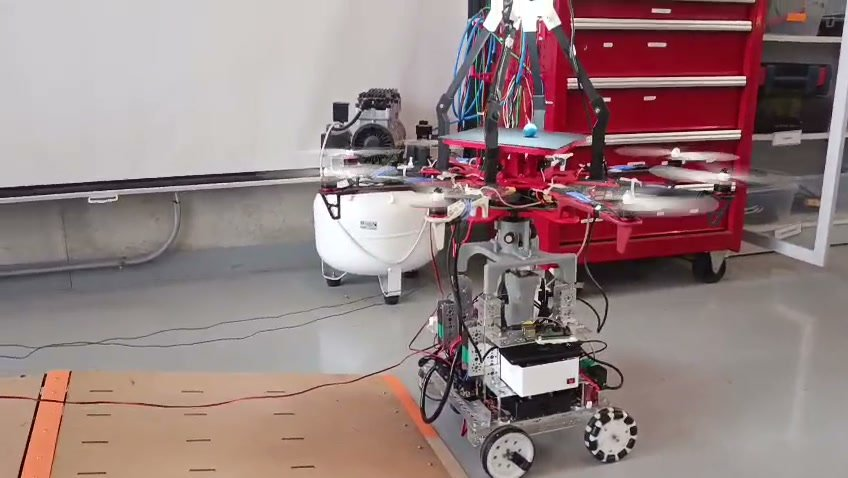
\includegraphics[width=\linewidth]{figures/photo_robot_side.jpg}\caption{Integrated prototype.}\end{subfigure}\hfill
  \begin{subfigure}[b]{0.30\textwidth}\centering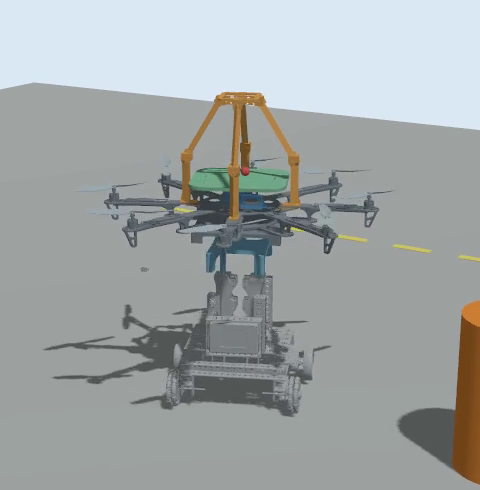
\includegraphics[width=\linewidth]{figures/cad_assembly.png}\caption{CAD assembly (383 parts).}\end{subfigure}\hfill
  \begin{subfigure}[b]{0.25\textwidth}\centering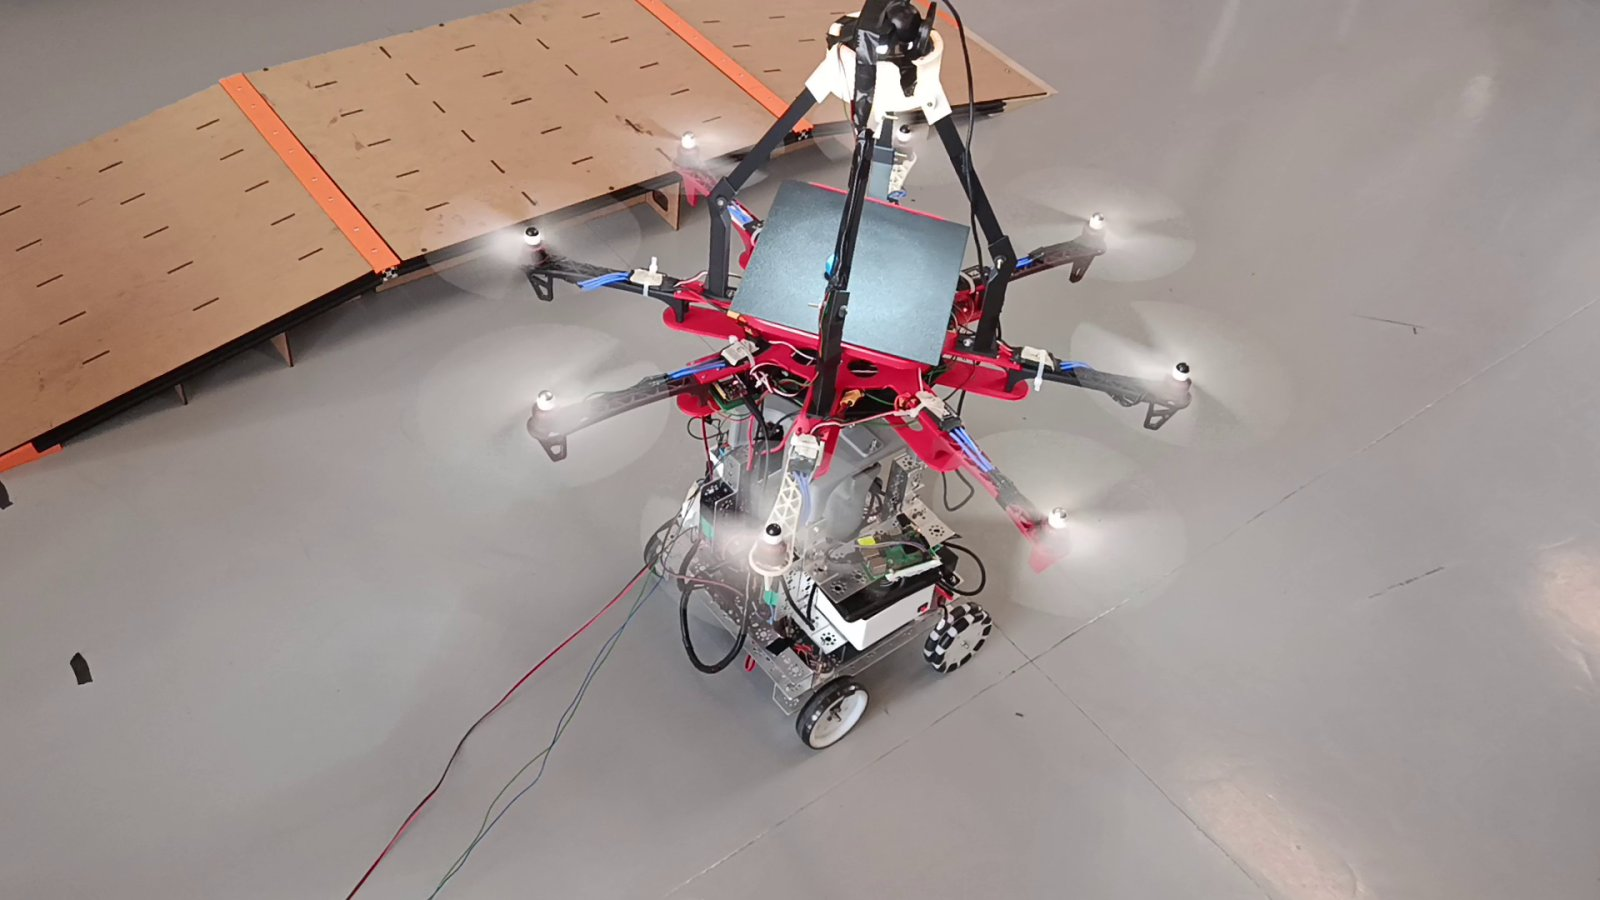
\includegraphics[width=\linewidth,trim=420 0 420 0,clip]{figures/photo_ramp_top.jpg}\caption{On the \SI{10}{\degree} ramp.}\end{subfigure}
  \caption{AeroTray. From bottom to top: TETRIX differential mobile base with myRIO, mast with vertical guide, spherical joint, octocopter (red frame, eight rotors), and ball-and-plate tray with overhead camera. The blue ball has a diameter of \SI{27}{\milli\metre}.}
  \label{fig:overview}
\end{figure}

\begin{enumerate}[label=\textbf{N\arabic*.}]
  \item \textbf{Mobile base.} TETRIX MAX aluminum chassis with two drive wheels (TETRIX TorqueNADO DC motors with quadrature encoders) and two omnidirectional wheels as passive supports. An NI myRIO-1900 reads the encoders, computes odometry, and executes a per-wheel PI velocity loop; an MDD10A H-bridge drives the motors from a \SI{12}{\volt} TETRIX NiMH battery. Track width $b=\SI{0.3794}{\metre}$; wheel travel per encoder count \SI{0.2151}{\milli\metre} (wheel radius $r\approx\SI{49.3}{\milli\metre}$).
  \item \textbf{Aerial module.} Octocopter with arms of radius $L=\SI{0.350}{\metre}$ (one motor every \SI{45}{\degree}), eight A2212 920\,KV brushless motors with 9450 propellers and 30\,A BEC-less ESCs, two 3S \SI{3300}{\milli\ampere\hour} LiPo batteries (one per group of four ESCs), an MPU-6050 IMU, and a VL53L0X time-of-flight sensor measuring distance to a matte-white target fixed to the base (Section~\ref{sec:altura}). A NodeMCU-32S (ESP32) runs attitude control at \SI{200}{\hertz}. The module mounts to the mast via a spherical joint on a carriage sliding along a vertical guide (measured travel of about \SI{140}{\milli\metre}); the spherical joint leaves roll and pitch free while friction and mechanical stops permit only a small yaw rotation, so the octocopter turns with the base. The moving assembly weighs \SI{3.6}{\kilo\gram} (\SI{3.3}{\kilo\gram} rotating assembly and \SI{0.3}{\kilo\gram} carriage). The rotor plane sits \SI{95}{\milli\metre} above the spherical joint center.
  \item \textbf{Ball-and-plate tray.} A $\SI{250}{\milli\metre}\times\SI{220}{\milli\metre}$ plate supported at its center on a universal joint atop a pillar fixed to the octocopter center plate, \SI{104}{\milli\metre} above the spherical joint, and tilted along two axes by two Futaba S3003 servos via four-bar linkages (Section~\ref{sec:linkage}). An ESP32-S3 generates the \SI{50}{\hertz} servo pulses (GPIO47 for $x$, GPIO21 for $y$) and runs the ball PID controller. A PS3 Eye camera, supported $\approx$\SI{0.20}{\metre} above the plate by four towers fixed to the octocopter (not the plate), streams $320\times240$ frames at \SI{187}{fps} to the Raspberry Pi, which detects the ball and sends its position and velocity to the ESP32-S3.
  \item \textbf{Supervisor, electronics distribution, and emergency stop.} The Raspberry Pi 3B+ centralizes vision, communications, and logging, with isolated logic domains and an emergency stop (Section~\ref{sec:power}). On the aerial module, both controllers mount beneath the center plate on opposite arms to balance weight and isolate ESC noise: the NodeMCU-32S (attitude control) on arm 8 ($+x$) and the ESP32-S3 (tray) on arm 6 ($-x$). The MPU-6050 IMU and VL53L0X laser sit beside the NodeMCU on arm 8 on the same I$^2$C bus, with the laser pointing down at the fixed target on the base. Both sensors are therefore offset from the spherical joint axis, and Section~\ref{sec:altura} corrects the height measurement for this lever arm.
\end{enumerate}

\begin{figure}[!htbp]
\centering
\begin{tikzpicture}[font=\footnotesize, >=Latex,
  colhdr/.style={font=\footnotesize\bfseries, text=pGris!85!black, align=center},
  blk/.style={draw, rounded corners=2pt, align=center, minimum height=11.5mm, inner xsep=2pt, inner ysep=2.5pt, line width=0.6pt},
  blkusr/.style={blk, fill=white, draw=pGris, text width=3.34cm},
  blkpw/.style={blk, fill=pRojo!7, draw=pRojo, text width=3.34cm},
  blkcp/.style={blk, fill=pAzul!7, draw=pAzul, text width=3.34cm},
  blksa/.style={blk, fill=pVerde!7, draw=pVerde, text width=4.04cm},
  pw/.style={->, line width=1.05pt, pRojo, rounded corners=2pt},
  pwbr/.style={pw, preaction={-, draw=white, line width=2.6pt, rounded corners=2pt}},
  dt/.style={<->, line width=0.85pt, pAzul, rounded corners=2pt},
  dt1/.style={->, line width=0.85pt, pAzul, rounded corners=2pt},
  lab/.style={font=\footnotesize, text=pAzul!90!black, inner sep=1.5pt}]
  % 3-column coordinates (total width = 13.38 cm < 13.74 cm = \textwidth)
  % Col 1: x=1.74 ([0.00, 3.48]), Col 2: x=6.28 ([4.54, 8.02]), Col 3: x=11.24 ([9.15, 13.33])
  \node[colhdr] at (1.74, -0.84) {Power};
  \node[colhdr] at (6.28, 0.90) {Compute};
  \node[colhdr] at (11.24, 0.90) {Sensors and actuators};

  % ---- Row 1 (y = 0.00) -- all boxes exactly 2 lines and equal height
  \node[blkusr] (web)  at (1.74,  0.00) {\textbf{Web browser}\\ laptop or phone};
  \node[blkcp]  (pi)   at (6.28,  0.00) {\textbf{Raspberry Pi 3B+}\\ vision, logging, web};
  \node[blksa]  (cam)  at (11.24, 0.00) {\textbf{PS3 Eye camera}\\ 320$\times$240 at 187 fps};

  % ---- Row 2 (y = -1.68)
  \node[blkpw]  (pipw) at (1.74, -1.68) {\textbf{BT5: 3S 18650}\\ XL4015 $\to$ 5.2 V};
  \node[blkcp]  (s3)   at (6.28, -1.68) {\textbf{ESP32-S3}\\ ball PID};
  \node[blksa]  (srv)  at (11.24,-1.68) {\textbf{2$\times$ Futaba S3003}\\ tray servos};

  % ---- Row 3 (y = -3.36)
  \node[blkpw]  (bt6)  at (1.74, -3.36) {\textbf{BT6: 3S 18650}\\ 5.2 V (servos, SB1)};
  \node[blksa]  (imu)  at (11.24,-3.36) {\textbf{MPU-6050, VL53L0X}\\ IMU and height laser};

  % ---- Row 4 (y = -5.04)
  \node[blkpw]  (lipo) at (1.74, -5.04) {\textbf{2$\times$ LiPo 3S}\\ 30 A fuses, K1, K2};
  \node[blkcp]  (nm)   at (6.28, -5.04) {\textbf{NodeMCU-32S}\\ attitude at 200 Hz};
  \node[blksa]  (esc)  at (11.24,-5.04) {\textbf{8$\times$ 30 A ESCs}\\ and drone motors};

  % ---- Row 5 (y = -7.08)
  \node[blkpw]  (bt4)  at (1.74, -7.08) {\textbf{BT4: power bank}\\ 5 V $\to$ 12 V boost};
  \node[blkcp]  (rio)  at (6.28, -7.08) {\textbf{NI myRIO-1900}\\ odometry, PI loop};
  \node[blksa]  (hb)   at (11.24,-7.08) {\textbf{MDD10A H-bridge}\\ 2$\times$TorqueNADO, enc.};

  % ---- Row 6 (y = -8.68)
  \node[blkpw]  (nimh) at (1.74, -8.68) {\textbf{12 V NiMH}\\ TETRIX, 20 A, K3};

  % ---- Data links (blue #0072B2)
  \draw[dt]  ([yshift=2.2mm]web.east) -- node[lab, above=1.5pt]{Wi-Fi} ([yshift=2.2mm]pi.west);
  \draw[dt]  (pi.east) -- node[lab, above=1.5pt]{USB} (cam.west);
  \draw[dt]  ([xshift=3mm]pi.south) -- node[lab, right=2pt]{USB} ([xshift=3mm]s3.north);
  \draw[dt1] (s3.east) -- node[lab, above=1.5pt]{PWM} (srv.west);

  % Pi <-> NodeMCU (USB) via left corridor of Col 2 and open Row 3 cell
  \draw[dt] ([xshift=-9mm]pi.south) -- ++(0,-0.42) -| (4.35,-3.36)
            -- node[lab, above=1.5pt, pos=0.55]{USB} (6.28,-3.36) -- (nm.north);
  % Pi <-> myRIO (UART 9600) via parallel corridor and open lane above myRIO
  \draw[dt] ([xshift=-13mm]pi.south) -- ++(0,-0.20) -| (3.98,-6.24)
            -- node[lab, above=1.5pt, pos=0.60]{UART 9600} (6.28,-6.24) -- (rio.north);

  % NodeMCU <-> IMU+VL53 (I2C) and NodeMCU -> ESC (PWM)
  \draw[dt]  ([xshift=10mm]nm.north) |- (8.05,-3.36) -- node[lab, above=1.5pt]{I$^2$C} (imu.west);
  \draw[dt1] (nm.east) -- node[lab, above=1.5pt]{PWM} (esc.west);
  % myRIO <-> MDD10A+TorqueNADO (PWM and encoders)
  \draw[dt1] ([yshift=2mm]rio.east) -- node[lab, above=1.5pt]{PWM} ([yshift=2mm]hb.west);
  \draw[dt1] ([yshift=-2mm]hb.west) -- node[lab, below=1.5pt]{enc.} ([yshift=-2mm]rio.east);

  % ---- Power links (red #D55E00)
  \draw[pw]   (pipw.east) -- (3.72,-1.68) |- ([yshift=-2.4mm]pi.west);
  \draw[pwbr] (bt6.east)  -- (3.72,-3.36) |- (3.72,-2.52) -| (srv.south);
  \draw[pwbr] (lipo.east) -- (3.72,-5.04) |- (3.72,-5.82) -| (esc.south);
  \draw[pw]   (bt4.east)  -- (rio.west);
  \draw[pw]   (nimh.east) -| (hb.south);

  % ---- Legend inside figure (centered below Row 6)
  \node[draw=pGris!60, rounded corners=2pt, fill=white, inner xsep=6pt, inner ysep=4pt, anchor=north]
    (leg) at (6.66,-9.48) {%
    \begin{tikzpicture}[baseline=-0.5ex, font=\footnotesize]
      \draw[dt]  (0.00,0) -- (0.58,0); \node[right=2.5pt, inner sep=0pt] at (0.58,0) {Data};
      \draw[pw]  (1.75,0) -- (2.33,0); \node[right=2.5pt, inner sep=0pt] at (2.33,0) {Power};
      \draw[fill=pRojo!7,  draw=pRojo,  rounded corners=1pt] (3.70,-0.12) rectangle (4.00,0.12);
      \node[right=2.5pt, inner sep=0pt] at (4.00,0) {Supplies};
      \draw[fill=pAzul!7,  draw=pAzul,  rounded corners=1pt] (5.70,-0.12) rectangle (6.00,0.12);
      \node[right=2.5pt, inner sep=0pt] at (6.00,0) {Compute};
      \draw[fill=pVerde!7, draw=pVerde, rounded corners=1pt] (7.82,-0.12) rectangle (8.12,0.12);
      \node[right=2.5pt, inner sep=0pt] at (8.12,0) {Sensors and actuators};
    \end{tikzpicture}};
\end{tikzpicture}
\caption{Electrical and communications architecture. Power domains share ground only through signal cables; the Raspberry Pi powers the camera, ESP32-S3, and NodeMCU-32S over USB. Pin assignments are listed in Table~\ref{tab:pins} and message frames in Section~\ref{sec:interfaces}.}
\label{fig:architecture}
\end{figure}

\subsection{Power system and emergency stop}
\label{sec:power}
Power distribution follows the Rev.~I electrical schematic (18 Nov 2026), released with the design files, and the group's power audit. Five independent power domains connect only through the signal grounds of the PWM and USB cables:
\begin{enumerate}[label=\textbf{S\arabic*.}]
  \item \textbf{Drone propulsion, two isolated branches.} Each 3S \SI{3300}{\milli\ampere\hour} 25C LiPo battery (BT1, BT2) runs through an XT60 connector, a \SI{30}{\ampere} ATO fuse (F1, F2), and contacts 30--87 of an automotive relay (K1, K2), then up to the drone via an $\approx$\SI{1}{\metre} 14\,AWG cable (loop resistance \SI{16.6}{\milli\ohm}) to a \SI{1000}{\micro\farad}/\SI{25}{\volt} capacitor per node. Branch A supplies ESCs 1, 3, 5, and 7 (M1, M3, M5, M7), and branch B supplies ESCs 2, 4, 6, and 8. Each branch drives two opposing pairs with two motors of each rotation direction, so an unevenly discharged battery lowers total thrust without producing yaw torque. Negative rails A$-$ and B$-$ join only on the drone (GND\_D), and the red BEC wire of every ESC is cut.
  \item \textbf{TETRIX base.} A \SI{12}{\volt} \SI{3000}{\milli\ampere\hour} NiMH pack (BT3), internal \SI{20}{\ampere} fuse, and relay K3 feed the MDD10A H-bridge ($2\times\SI{10}{\ampere}$) and both TorqueNADO motors.
  \item \textbf{myRIO.} A \SI{5}{\volt}/\SI{3}{\ampere} power bank (BT4) and a 5-to-\SI{12}{\volt} boost converter supply the myRIO, which powers the encoders.
  \item \textbf{\SI{5}{\volt} logic} (root of the ground tree). A 3S 18650 pack with BMS (BT5), \SI{3}{\ampere} fuse, switch SW1, and XL4015 regulator set to \SI{5.2}{\volt} powers the Raspberry Pi and, through the USB hub, the NodeMCU-32S (with its sensors) and the ESP32-S3.
  \item \textbf{Servos and emergency stop.} A second 3S 18650 pack with BMS (BT6), \SI{3}{\ampere} fuse, SW2, and XL4015 feeds both S3003 servos (with \SI{1000}{\micro\farad} and $2\times\SI{100}{\micro\farad}$ capacitors) and the LED ring. Through a \SI{1}{\ampere} fuse and a \SI{4}{\metre} two-conductor cable, the same pack energizes relay coils K1--K4 via the latching normally closed mushroom emergency stop (SB1) on the control box; each coil carries a 1N4007 flyback diode. Pressing SB1 simultaneously opens both LiPo branches, the base battery, and servo power (K4), while logic remains powered and logging.
\end{enumerate}
In hover, each branch delivers 18--\SI{22}{\ampere} (60--75\% of the fuse rating; Section~\ref{sec:bateria}). Above \SI{1850}{\micro\second}, current approaches \SI{30}{\ampere}, so the firmware restricts operation in that band to \SI{20}{\second}. The Rev.~I schematic omits battery sensing: although the Rev.~E wiring diagram shows \SI{10}{\kilo\ohm}/\SI{3.3}{\kilo\ohm} dividers to GPIO34 and GPIO35, firmware v11 does not read them, and LiPo voltages are measured manually before and after each session (Section~\ref{sec:operation}).

\subsection{Pin assignments}
\label{sec:pins}
Some earlier project documents (previous wiring diagrams and the power audit's proposal to relocate ESC4 and ESC7) diverge from the code. Table~\ref{tab:pins} follows the flight firmware released in \fn{03_firmware}.

\begin{table}[!htbp]
\centering
\caption{Embedded controller pin assignments per the flight firmware: drone v11 and ESP32-S3 ball PID (folder \texttt{03\_firmware}).}
\label{tab:pins}
\small
\begin{tabularx}{\textwidth}{@{}llX@{}}
\toprule
Controller & Pin & Function \\
\midrule
NodeMCU-32S (U10) & GPIO25, 27, 21, 5 & \SI{50}{\hertz} PWM for M1, M3, M5, M7 (branch A) \\
 & GPIO26, 14, 19, 17 & \SI{50}{\hertz} PWM for M2, M4, M6, M8 (branch B) \\
 & GPIO23 / GPIO22 & I$^2$C SDA / SCL at \SI{100}{\kilo\hertz}: MPU-6050 (0x68) and VL53L0X (0x29) \\
 & GPIO34 / GPIO35 & VBAT\_A / VBAT\_B via $\div4.03$ divider (wired in Rev.~E; unused by firmware v11) \\
 & USB & \SI{5}{\volt}, commands, heartbeat, and telemetry with the Raspberry Pi \\
ESP32-S3 (U16) & GPIO47 / GPIO21 & $x$-servo / $y$-servo pulse (\SI{50}{\hertz}, neutral 1386/\SI{1392}{\micro\second}, $\pm\SI{220}{\micro\second}$) \\
Raspberry Pi 3B+ & GPIO14 / GPIO15 & UART TX / RX to myRIO MXP-A pin 10 (RX) / pin 14 (TX), 9600 8N1 \\
myRIO-1900 & MXP-A, MXP-B & PWM and DIR to MDD10A and encoder inputs (left motor on MXP-A, right on MXP-B); UART on MXP-A \\
\bottomrule
\end{tabularx}
\end{table}

GPIO5 and GPIO14 output glitch pulses during ESP32 boot. As long as ESCs remain on those pins, the LiPo branches are energized (releasing SB1 to close K1 and K2) only after the NodeMCU has booted and is outputting \SI{1000}{\micro\second} to all ESCs.

\subsection{Supervisor and interfaces}
\label{sec:interfaces}
The Raspberry Pi 3B+ serves as the system hub. Its program (\texttt{seguidor.py}) performs five functions:
\begin{itemize}
  \item captures raw YUYV frames from the PS3 Eye at \SI{187}{fps}, rectifies the plate with a four-corner homography, and detects the ball by color with OpenCV \cite{bradski2000};
  \item streams ball position and velocity to the ESP32-S3 over USB serial (frame \texttt{p x,y,vx,vy});
  \item exchanges commands, a heartbeat (\texttt{hb}), and telemetry with the octocopter over USB serial;
  \item communicates with the myRIO over the hardware UART on the GPIO header;
  \item logs all streams to CSV files and serves three web pages: \texttt{/} (ball and plate), \texttt{/dron} (octocopter), and \texttt{/robot} (full robot).
\end{itemize}
The myRIO and Pi exchange two text frames at 9600\,baud, 8N1:
\begin{itemize}
  \item from myRIO to Pi, \texttt{cmd1,cmd2}, where codes 1--4 command the octocopter and codes 5--11 command the ball-and-plate stage;
  \item from Pi to myRIO, every \SI{50}{\milli\second}, \texttt{x,y,roll,pitch,uav,bp}.
\end{itemize}
Commands received from the myRIO take priority over web commands for \SI{250}{\milli\second}.

\subsection{Design decisions and modifications}
The final configuration emerged from several iterations; the key decisions are:
\begin{itemize}
  \item \textbf{A drone rather than a gimbal on the base.} The octocopter fulfills two roles a motorized gimbal cannot achieve simultaneously: it levels relative to gravity, eliminating ground slope from the ball dynamics (Section~\ref{sec:chain}), and it supports part of its own weight, lowering the robot's effective center of mass on a ramp and reducing climbing torque (Section~\ref{sec:porquedron}).
  \item \textbf{Passive spherical joint instead of free flight.} A spherical joint on a vertical guide allows the octocopter to balance in roll and pitch and lift a few centimeters while remaining captive; this ensures indoor safety and preserves the mechanical base coupling under study.
  \item \textbf{Eight rotors.} With 8 motors, the \SI{3.6}{\kilo\gram} assembly hovers on charged batteries at 1725--\SI{1775}{\micro\second} (68--74\% of the usable map range), allowing the mixer to trade collective thrust for attitude torque (Section~\ref{sec:aerial}). Thrust margin depends strongly on battery voltage (Section~\ref{sec:bateria}).
  \item \textbf{Camera on the Pi instead of on the ESP32.} The first version used a camera on the ESP32-S3, limited to about 50\,fps by JPEG compression (lowering JPEG quality caused hundreds of corrupt frames per minute). Switching to a PS3 Eye on the Pi raised the rate to \SI{187}{fps} with uncompressed frames, making velocity estimation and the ball PID derivative term usable; remaining loop delay sets the derivative-gain ceiling (Section~\ref{sec:ballcontrol}).
  \item \textbf{Isolated power domains.} Each subsystem has its own supply and domains share only ground (Section~\ref{sec:power}). The original BMS for servos and relay coils failed during testing and was replaced by a bench supply in part of the trials (Section~\ref{sec:limits}).
  \item \textbf{Flight firmware iterations.} Nine guided-flight trials led to firmware v9 (Section~\ref{sec:flights}): an accelerometer low-pass filter against rotor vibration, an active yaw loop, a larger angle-integral term, a wider in-flight angular-rate command limit, and hysteresis in flight-gain switching. The model in Section~\ref{sec:authority} explains why the decisive change was the angular-rate command limit rather than the gains. The final v11 release added a sliding yaw window at idle for base turns and a Kalman filter with cascaded altitude control over the calibrated laser (Section~\ref{sec:altura}).
\end{itemize}
         % 2. Hardware description (incl. power and pins)
%% ======================================================================
%% 04a_kinematics.tex -- 3. Model (part 1): assumptions, frames, parameters, kinematics
%% Symbolic verification: scripts_modelo/derive_*.py ; numbers: scripts_modelo/analysis.py
%% ======================================================================
\section{Kinematic and dynamic model}
\label{sec:model}

This section derives the model of the full chain---base $\to$ spherical joint $\to$ octocopter $\to$ plate $\to$ ball---used to size the prototype, design and diagnose its three controllers, and interpret the experiments in Section~\ref{sec:validation}. The derivation proceeds from the bottom up: assumptions, frames, and parameters (Section~\ref{sec:assumptions}); kinematics of the base, the full chain, and the plate actuation (Sections~\ref{sec:basekin}--\ref{sec:linkage}); dynamics of the base, the octocopter, and the ball (Sections~\ref{sec:basedyn}--\ref{sec:ball}); the rationale for using a drone on the ramp and its thrust margin versus battery voltage (Sections~\ref{sec:porquedron}--\ref{sec:bateria}); and finally, the coupled linear model, the controllers, and the resulting fundamental limitations (Sections~\ref{sec:coupling}--\ref{sec:limits_fund}). Every equation for the ball and octocopter dynamics was verified symbolically in SymPy, and all numerical values in this section are computed by the scripts in \fn{scripts_modelo/} in the repository (\ref{app:derivations}).

\subsection{Assumptions, frames, and parameters}
\label{sec:assumptions}

\paragraph{Modeling assumptions}
\begin{enumerate}[label=\textbf{A\arabic*.}, leftmargin=*]
  \item All links are rigid; the compliance of the PLA plates and towers is neglected.
  \item The driven wheels roll without longitudinal or lateral slip; the omnidirectional wheels are passive supports with negligible lateral resistance.
  \item The spherical joint is ideal in roll and pitch; its friction torque $\vect{\tau}_f$ is treated as an unmodeled disturbance. Its yaw is locked by friction and mechanical stops, so the octocopter heading follows the base (confirmed by the yaw cutoffs in Section~\ref{sec:integrated}).
  \item The vertical guide is a prismatic joint with Coulomb and viscous friction $F_g(\dot d)$ and rigid end stops at $d=0$ and $d=d_{\max}$.
  \item Each rotor produces thrust $F_i$ along $+\vect{z}_D$ and a proportional reaction torque; the ESC--motor--propeller assembly responds to its command with a pure time delay followed by a first-order lag $\tau_m$. Thrust at a fixed command scales with the square of the voltage reaching the ESCs (Section~\ref{sec:bateria}).
  \item The ball is a homogeneous sphere rolling without slip; rolling resistance is neglected. The inertia factor $\gamma_b=1/(1+I_b/m_br_b^2)$ is kept general ($\gamma_b=5/7$ for a solid sphere, $3/5$ for a thin spherical shell).
  \item The servos are position servos with a pure time delay and a first-order lag; linkage backlash is treated as a nonlinearity outside the linear model.
  \item For linear analysis, angles, angular rates, and accelerations are small, and the base moves at constant slope except at the ramp transitions.
\end{enumerate}

\paragraph{Frames and notation}
Figure~\ref{fig:frames} shows the coordinate frames. $\{W\}$ is an inertial frame with $\vect z_W$ pointing upward. $\{B\}$ is fixed to the base, with its origin on the ground below the midpoint of the driven (rear) axle, $\vect x_B$ pointing forward (toward the omnidirectional wheels), and $\vect z_B$ normal to the ground. $\{J\}$ has its origin at the center of the spherical joint, at height $h_{J0}+d$ above the ground and distance $\ell_J$ ahead of the driven axle, where $d\in[0,d_{\max}]$ is the displacement along the vertical guide. $\{D\}$ is fixed to the octocopter with its origin at the spherical joint center, $\vect x_D$ toward motor M8, $\vect y_D$ toward motor M7, and $\vect z_D$ upward (the firmware FLU convention). $\{G\}$ is fixed to the octocopter at the center of the plate universal joint, at height $h_P$ along $\vect z_D$. $\{P\}$ is the plate frame, with its origin at the universal joint center; the ball center has coordinates $\vect\rho=[x_b,\,y_b,\,\varepsilon]\T$ in $\{P\}$, where $\varepsilon$ is the height of the ball center above the universal joint center. $\Rot_x,\Rot_y,\Rot_z$ are elementary rotations, $\skw{\vect a}$ is the skew-symmetric matrix of $\vect a$, and orientations use the $z$--$y$--$x$ Euler angles $(\psi,\theta,\phi)$ implemented in the firmware. A vector without a superscript is expressed in the frame specified in the text; $\vect a^{B}$ denotes components in $\{B\}$.

The robot configuration is described by
\begin{equation}
  \vect{q}=\big[\,x,\ y,\ \psi\ \big|\ d\ \big|\ \phi,\ \theta,\ \psi_D\ \big|\ \alpha_x,\ \alpha_y\ \big|\ x_b,\ y_b\,\big]\T\in\mathbb{R}^{11},
  \label{eq:q}
\end{equation}
where $(x,y,\psi)$ is the planar pose of the base in the ground plane, $d$ is the vertical guide displacement, $(\phi,\theta,\psi_D)$ are the roll, pitch, and heading of the octocopter relative to $\{W\}$, $(\alpha_x,\alpha_y)$ are the servo-driven plate tilt angles relative to $\{D\}$, and $(x_b,y_b)$ is the ball position on the plate. The yaw lock in A3 eliminates $\psi_D$ and leaves ten configuration coordinates; the base is subject to one nonholonomic constraint (Section~\ref{sec:basekin}), so the robot has nine velocity degrees of freedom, while the ball's rolling constraints fix its angular velocity in terms of $(\dot x_b,\dot y_b)$ (Section~\ref{sec:ball}). Seven actuation channels drive these nine degrees of freedom (two wheels; the eight rotors, acting as one collective and two torques; two servos), while two coordinates, $(x_b,y_b)$, are unactuated.

\begin{figure}[!htbp]
\centering
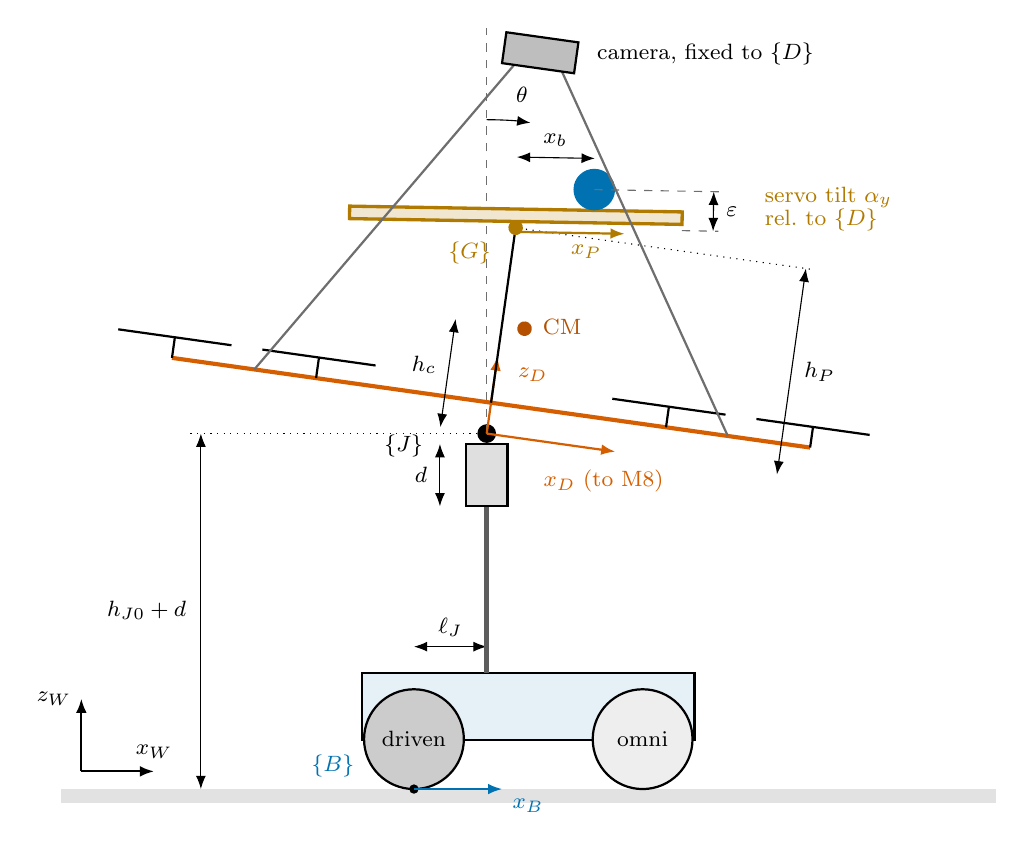
\begin{tikzpicture}[scale=1.32, font=\footnotesize, ax/.style={-{Latex[length=1.8mm]}, thick}]
  % ground and world frame
  \fill[pGris!20] (-4.5,-0.32) rectangle (4.5,-0.45);
  \draw[ax] (-4.3,-0.15) -- (-3.6,-0.15) node[above=1pt]{$x_W$};
  \draw[ax] (-4.3,-0.15) -- (-4.3,0.55) node[left]{$z_W$};
  % base: driven (rear) wheel and omni (front) wheel
  \draw[thick, fill=pAzul!10] (-1.6,0.15) rectangle (1.6,0.8);
  \draw[thick, fill=pGris!35] (-1.1,0.16) circle (0.48); \draw[thick, fill=pGris!12] (1.1,0.16) circle (0.48);
  \node at (-1.1,0.16) {driven}; \node at (1.1,0.16) {omni};
  \fill (-1.1,-0.32) circle (0.045);
  \draw[ax, pAzul] (-1.1,-0.32) -- (-0.25,-0.32) node[below right]{$x_B$};
  \node[pAzul] at (-1.88,-0.10) {$\{B\}$};
  % mast offset l_J
  \draw[{Latex}-{Latex}] (-1.1,1.05) -- (-0.4,1.05); \node[above] at (-0.75,1.05) {$\ell_J$};
  \draw[line width=2pt, pGris!85!black] (-0.4,0.8) -- (-0.4,3.0);
  \draw[thick, fill=pGris!22] (-0.6,2.4) rectangle (-0.2,3.0);
  \draw[{Latex}-{Latex}] (-0.85,2.4) -- (-0.85,3.0); \node[left] at (-0.88,2.7) {$d$};
  \draw[{Latex}-{Latex}] (-3.15,-0.32) -- (-3.15,3.1); \node[left] at (-3.20,1.4) {$h_{J0}+d$};
  \draw[dotted] (-3.25,3.1) -- (-0.5,3.1);
  % joint
  \fill (-0.4,3.1) circle (0.09); \node[below left] at (-0.92,3.18) {$\{J\}$};
  \draw[dashed, pGris] (-0.4,3.1) -- (-0.4,7.0);
  % octocopter pitched by theta (all lengths in its own frame)
  \begin{scope}[shift={(-0.4,3.1)}, rotate=-8]
    \draw[line width=1.5pt, pRojo] (-3.1,0.3) -- (3.1,0.3);
    \foreach \xx in {-3.1,-1.7,1.7,3.1} {\draw[thick] (\xx,0.3) -- (\xx,0.5); \draw[thick] (\xx-0.55,0.5) -- (\xx+0.55,0.5);}
    \draw[ax, pRojo] (0,0) -- (1.25,0); \node[pRojo, below] at (1.15,-0.10) {$x_D$ (to M8)};
    \draw[ax, pRojo] (0,0) -- (0,0.75); \node[pRojo] at (0.36,0.62) {$z_D$};
    % centre of mass
    \fill[pRojo!85!black] (0.22,1.05) circle (0.07); \node[right, pRojo!85!black] at (0.30,1.08) {CM};
    \draw[{Latex}-{Latex}] (-0.45,0) -- (-0.45,1.05); \node[left] at (-0.48,0.6) {$h_c$};
    % pillar, universal joint G and plate
    \draw[thick] (0,0.3) -- (0,1.95);
    \fill[pOcre] (0,2.0) circle (0.07); \node[below left, pOcre] at (-0.14,1.94) {$\{G\}$};
    \draw[{Latex}-{Latex}] (2.82,0) -- (2.82,2.0); \node[right] at (2.85,1.0) {$h_P$};
    \draw[dotted] (0.1,2.0) -- (2.88,2.0);
    \begin{scope}[shift={(0,2.0)}, rotate=7]
      \draw[very thick, pOcre, fill=pOcre!18] (-1.6,0.06) rectangle (1.6,0.18);
      \fill[pAzul] (0.75,0.38) circle (0.2);
      \draw[ax, pOcre] (0,-0.04) -- (1.05,-0.04); \node[pOcre, below] at (0.68,-0.06) {$x_P$};
      \draw[pGris, dashed] (0.75,0.38) -- (1.95,0.38); \draw[pGris, dashed] (1.6,0) -- (1.95,0);
      \draw[{Latex}-{Latex}] (1.9,0) -- (1.9,0.38); \node[right] at (1.93,0.19) {$\varepsilon$};
      \draw[{Latex}-{Latex}] (0,0.68) -- (0.75,0.68); \node[above] at (0.37,0.69) {$x_b$};
      \node[pOcre, right, align=left] at (2.30,0.22) {servo tilt $\alpha_y$\\[-1pt]rel.\ to $\{D\}$};
    \end{scope}
    % camera towers (fixed to the drone)
    \draw[thick, pGris] (-2.3,0.3) -- (-0.2,3.6); \draw[thick, pGris] (2.3,0.3) -- (0.2,3.6);
    \draw[thick, fill=pGris!45] (-0.35,3.55) rectangle (0.35,3.85); \node[right] at (0.45,3.75) {camera, fixed to $\{D\}$};
  \end{scope}
  \draw[-{Latex}] (-0.4,6.12) arc (90:82:3.02); \node at (-0.06,6.36) {$\theta$};
\end{tikzpicture}
\caption{Coordinate frames and lengths of the kinematic chain in the $x$--$z$ plane (pitch $\theta$ is shown; roll is analogous about $x$). Frame $\{D\}$ has its origin at the spherical joint center $\{J\}$. The camera towers are fixed to the octocopter, so the camera measures the ball in a frame that tilts with the octocopter but not with the servos.}
\label{fig:frames}
\end{figure}

\paragraph{Parameters}
Table~\ref{tab:params} summarizes the model parameters and their sources. Dimensions come from the CAD assembly of the final prototype (383 parts); masses from weighing; actuator specifications from datasheets; gains from firmware; and three quantities ($\delta_x,\delta_y$, $h_c$, and $k_F$) are identified from flight logs in Section~\ref{sec:ident}.

\begin{small}
\begin{longtable}{@{}>{\raggedright\arraybackslash}p{0.16\textwidth}>{\raggedright\arraybackslash}p{0.43\textwidth}>{\raggedleft\arraybackslash}p{0.35\textwidth}@{}}
\caption{Model parameters. Sources: [CAD] assembly model; [M] measured; [DS] datasheet; [FW] firmware or LabVIEW code; [ID] identified in this work; [E] engineering estimate.}\label{tab:params}\\
\toprule
Symbol & Description & Value [source] \\
\midrule\endfirsthead
\toprule Symbol & Description & Value [source] \\ \midrule\endhead
\multicolumn{3}{@{}l}{\emph{Mobile base}}\\
$r$, $b$, $L$ & wheel radius, track width, wheelbase & \SI{49.3}{\milli\metre}, \SI{0.3794}{\metre}, \SI{0.220}{\metre} [FW, M] \\
$\kappa_e$ & wheel travel per encoder count (1440 counts/rev) & \SI{0.2151}{\milli\metre} [FW, DS] \\
$\tau_s$, $\omega_0$, $i_s$ & TorqueNADO stall torque, no-load speed, and stall current (12\,V, 60:1) & \SI{4.94}{\newton\metre}, \SI{100}{rpm}, \SI{8.7}{\ampere} [DS] \cite{pitsco_torquenado} \\
$M$ & total robot mass with all batteries (remainder \SI{6.8}{\kilo\gram} + module \SI{3.6}{\kilo\gram}) & \SI{10.4}{\kilo\gram} [M] \\
$x_G$, $h_G$ & CM ahead of driven axle and above support plane, from measured tip-over slopes (\SI{21.5}{\degree} and \SI{30.5}{\degree}, module locked) & \SI{0.088}{\metre}, \SI{0.224}{\metre} [M] \\
$\ell_J$, $h_{J0}$, $d_{\max}$ & mast offset, spherical joint height at $d=0$, guide stroke & \SI{0.088}{\metre}, \SI{0.495}{\metre}, \SI{0.140}{\metre} [CAD, M] \\
$C_{rr}$ & rolling resistance coefficient & 0.02 [E] \\
\midrule
\multicolumn{3}{@{}l}{\emph{Aerial module}}\\
$m$, $m_c$ & rotating assembly, carriage & \SI{3.3}{\kilo\gram}, \SI{0.3}{\kilo\gram} [M] \\
$\vect J$ & inertia about spherical joint center & $\diag(0.12;\ 0.12;\ 0.20)$\,\si{\kilo\gram\metre\squared} [CAD] \\
$h_c$ & CM height above spherical joint & $0.14\pm0.06$\,m [ID]; 0.10\,m [CAD] \\
$\delta_x$, $\delta_y$ & horizontal CM eccentricity & $9.5\pm1.8$\,mm, $1.9\pm1.5$\,mm [ID] \\
$L_r$, $h_r$ & rotor radius, rotor plane above spherical joint & \SI{0.350}{\metre}, \SI{0.095}{\metre} [CAD] \\
$(x_i,y_i)$, M1--M4 & rotor positions, clockwise ($s_i=-1$) & $(D,-D)$, $(-D,-D)$, $(-D,D)$, $(D,D)$, $D=L_r/\sqrt2$ [FW] \\
$(x_i,y_i)$, M5--M8 & rotor positions, counterclockwise ($s_i=+1$) & $(0,-L_r)$, $(-L_r,0)$, $(0,L_r)$, $(L_r,0)$ [FW] \\
$k_F$, $u_0$, $n$ & thrust map $F=k_F((u-u_0)/\SI{860}{\micro\second})^n$ & 5.40\,N [FW], 7.17--8.18\,N [ID] at 12.4\,V; \SI{1140}{\micro\second}; 1.6 \\
$c_Q$ & reaction torque per unit thrust & \SI{0.020}{\metre} [FW] \\
$\tau_m$, $T_a$ & motor--ESC lag, actuation delay (50\,Hz ESC frame, IMU filter) & \SI{0.07}{\second} [E], \SI{0.02}{\second} [FW] \\
$C_b$, $R_\Sigma$ & capacity per 3S LiPo; internal + cable + contact resistance per branch & \SI{3.3}{\ampere\hour} [DS]; 41--\SI{68}{\milli\ohm} [E, audit] \\
\midrule
\multicolumn{3}{@{}l}{\emph{Ball and plate}}\\
$h_P$ & universal joint center above spherical joint & \SI{0.104}{\metre} [CAD] \\
$\varepsilon$, $r_b$ & ball center height above universal joint, ball radius & \SI{36.9}{\milli\metre}, \SI{13.5}{\milli\metre} [CAD, M] \\
$r_a$, $\ell_r$, $R_h$ & servo arm, connecting rod, and linkage horn radius & 20, 36, \SI{45.85}{\milli\metre} [CAD] \\
$k_s$ & servo gain (S3003: \SI{45}{\degree} per \SI{400}{\micro\second}) & \SI{0.1125}{\degree\per\micro\second} [DS] \cite{futaba_s3003} \\
$K_\alpha$ & plate tilt per microsecond of pulse width & \SI{0.0491}{\degree\per\micro\second} [CAD, DS] \\
$H_c$ & camera height above plate & \SI{0.20}{\metre} [CAD] \\
\bottomrule
\end{longtable}
\end{small}

\subsection{Differential base kinematics}
\label{sec:basekin}

Let $v$ and $\omega$ be the linear and angular velocities of $\{B\}$, and let $\omega_R,\omega_L$ be the angular velocities of the right and left wheels. By A2, the velocity of the axle midpoint has no lateral component, yielding the Pfaffian (nonholonomic) constraint
\begin{equation}
  \big[-\sin\psi\ \ \cos\psi\ \ 0\big]\,\big[\dot x\ \ \dot y\ \ \dot\psi\big]\T=0,
  \label{eq:pfaff}
\end{equation}
and the kinematic model \cite{siegwart2011,campion1996}
\begin{equation}
  \begin{bmatrix}\dot x\\ \dot y\\ \dot\psi\end{bmatrix}=\begin{bmatrix}\cos\psi&0\\ \sin\psi&0\\ 0&1\end{bmatrix}\begin{bmatrix}v\\ \omega\end{bmatrix},\qquad
  \begin{bmatrix}v\\ \omega\end{bmatrix}=\begin{bmatrix}r/2 & r/2\\ r/b & -r/b\end{bmatrix}\begin{bmatrix}\omega_R\\ \omega_L\end{bmatrix},
  \label{eq:diff}
\end{equation}
whose inverse, used on the myRIO, is $v_{R,L}=r\omega_{R,L}=v\pm\tfrac{b}{2}\omega$, with $b/2=\SI{0.1897}{\metre}$. The instantaneous center of rotation lies on the axle line at distance $R_c=\tfrac{b}{2}\,(\omega_R+\omega_L)/(\omega_R-\omega_L)$ from the midpoint. The two turns specified in the course guide are therefore pivoting about the axle midpoint ($\omega_L=-\omega_R$, $R_c=0$, $\omega=2v_R/b$) and pivoting about one wheel ($\omega_L=0$, $R_c=b/2$, $\omega=v_R/b$). Because the spherical joint lies a distance $\ell_J$ ahead of the axle, it traces a circle of radius $\ell_J=\SI{0.088}{\metre}$ in the first case and $\sqrt{(b/2)^2+\ell_J^2}=\SI{0.209}{\metre}$ in the second; Section~\ref{sec:coupling} shows that the resulting centripetal accelerations are negligible.

\paragraph{Odometry}
The LabVIEW node integrates the encoder increments $\Delta N_{R,L}$ at each sample period using the midpoint rule:
\begin{gather}
  \Delta s_{R,L}=\kappa_e\,\Delta N_{R,L},\qquad \Delta s=\tfrac12(\Delta s_R+\Delta s_L),\qquad \Delta\psi=\frac{\Delta s_R-\Delta s_L}{b},\\
  \begin{bmatrix}x\\y\end{bmatrix}_{k+1}=\begin{bmatrix}x\\y\end{bmatrix}_{k}+\Delta s\begin{bmatrix}\cos(\psi_k+\Delta\psi/2)\\ \sin(\psi_k+\Delta\psi/2)\end{bmatrix},\qquad \psi_{k+1}=\psi_k+\Delta\psi .
  \label{eq:odo}
\end{gather}
For constant wheel velocities within a sample period, the exact (circular-arc) update multiplies the increment by $\operatorname{sinc}(\Delta\psi/2)=1-\Delta\psi^2/24+O(\Delta\psi^4)$, so the truncation error of \eqref{eq:odo} is $\Delta s\,\Delta\psi^2/24$ per step---under \SI{1}{\nano\metre} at the operating speeds ($|\omega|\le\SI{0.5}{\radian\per\second}$, \SI{10}{\milli\second} period). Resolution is one count: $\kappa_e=\SI{0.2151}{\milli\metre}$ in translation and $\kappa_e/b=\SI{0.57}{\milli\radian}$ ($0.032^\circ$) in heading. The dominant odometry errors are therefore systematic \cite{borenstein1996}: a relative difference $\epsilon_d$ between wheel radii produces a heading drift $\epsilon_d S/b$ and a lateral offset $\epsilon_d S^2/(2b)$ over a straight run of length $S$ (\SI{1.5}{\degree} and \SI{13}{\milli\metre} per meter for $\epsilon_d=1\%$), and a relative track-width error $\epsilon_b$ produces a heading error $-\epsilon_b\Theta$ over an in-place turn $\Theta$. Both are calibrated with the 1\,m and 360$^\circ$ tests in Section~\ref{sec:integrated}.

\subsection{Slope embedding and kinematic chain}
\label{sec:chain}

Let the ground be a plane of slope $\beta$ whose direction of steepest ascent is $\vect x_W$. With $(x,y,\psi)$ measured in that plane, the base pose is
\begin{equation}
  \Rot_{WB}=\Rot_y(-\beta)\,\Rot_z(\psi),\qquad \vect p_{B}=\Rot_y(-\beta)\,[x\ \ y\ \ 0]\T ,
  \label{eq:slope}
\end{equation}
and gravity, expressed in $\{B\}$, is
\begin{equation}
  \vect g^{B}=\Rot_{WB}\T\begin{bmatrix}0\\0\\-g\end{bmatrix}=g\begin{bmatrix}-\sin\beta\cos\psi\\ \sin\beta\sin\psi\\ -\cos\beta\end{bmatrix}.
  \label{eq:gB}
\end{equation}
The positions of the spherical joint, universal joint, and ball follow from the chain of homogeneous transformations:
\begin{align}
  \vect p_J&=\vect p_B+\Rot_{WB}\big[\ell_J\ \ 0\ \ h_{J0}+d\big]\T, \label{eq:pJ}\\
  \vect p_G&=\vect p_J+\Rot_{WD}\,h_P\ez,\qquad \Rot_{WD}=\Rot_z(\psi_D)\Rot_y(\theta)\Rot_x(\phi), \label{eq:pG}\\
  \vect p_b&=\vect p_G+\Rot_{WD}\Rot_{DP}\,\vect\rho,\qquad \Rot_{DP}=\Rot_y(\alpha_y)\Rot_x(\alpha_x),\qquad \vect\rho=[x_b\ \ y_b\ \ \varepsilon]\T . \label{eq:pb}
\end{align}
Two properties of \eqref{eq:pG}--\eqref{eq:pb} shape the entire design. First, $(\phi,\theta)$ are \emph{absolute} angles: the octocopter IMU estimates them relative to gravity and its controller drives them to zero. To first order, the absolute tilt of the plate is
\begin{equation}
  \Theta_P\simeq\theta+\alpha_y,\qquad \Phi_P\simeq\phi+\alpha_x ,
  \label{eq:tilt}
\end{equation}
which does not contain the slope $\beta$: the passive spherical joint and self-leveling octocopter decouple ground slope from the plate. If the tray were fixed to the base, the plate would tilt by $\arcsin(\sin\beta\cos\psi)$; on the \SI{10}{\degree} ramp the servos would spend \SI{10}{\degree} of their \SI{\pm10.8}{\degree} stroke (Section~\ref{sec:linkage}) just to level it, and on a \SI{20}{\degree} ramp they could not level it at all. Second, the ball sits at height $h_P+\varepsilon=\SI{0.141}{\metre}$ above the spherical joint, a lever arm that converts octocopter angular accelerations into linear ball accelerations.

\paragraph{Velocity and acceleration propagation}
With $\vect r_{BJ}=[\ell_J,0,h_{J0}+d]\T$, base angular velocity and acceleration $\vect\omega_B,\vect\alpha_B$, and octocopter body-frame angular rates $\vect\omega_D=[p,q,r]\T$, the accelerations of the spherical joint and universal joint are
\begin{align}
  \vect a_J&=\vect a_B+\vect\alpha_B\times\vect r_{BJ}+\vect\omega_B\times(\vect\omega_B\times\vect r_{BJ})+2\,\vect\omega_B\times\dot d\,\ez+\ddot d\,\ez, \label{eq:aJ}\\
  \vect a_G&=\vect a_J+\vect\alpha_D\times h_P\ez+\vect\omega_D\times(\vect\omega_D\times h_P\ez). \label{eq:aG}
\end{align}
For planar motion on a constant slope ($\vect\omega_B=\omega\,\vect z_B$) and $\ddot d=0$, \eqref{eq:aJ} reduces in $\{B\}$ to
\begin{equation}
  \vect a_J^{B}=\big[\dot v-\omega^2\ell_J,\ \ v\omega+\dot\omega\,\ell_J,\ \ 0\big]\T ,
  \label{eq:aJplanar}
\end{equation}
because the axle midpoint acceleration of a nonholonomic base is $[\dot v,\ v\omega,\ 0]\T$. Terms with $\vect\omega_B\times$ and $\vect\alpha_B\times$ in the vertical plane appear only at the ramp transitions, where the base pitches and the spherical joint, \SI{0.5}{\metre} above the ground, experiences the tangential acceleration $(h_{J0}+d)\,\ddot\theta_B$. The octocopter Euler-angle derivatives relate to body angular velocities via
\begin{equation}
  \dot\phi=p+\tan\theta\,(q\sin\phi+r\cos\phi),\quad \dot\theta=q\cos\phi-r\sin\phi,\quad \dot\psi_D=\frac{q\sin\phi+r\cos\phi}{\cos\theta},
  \label{eq:euler_rates}
\end{equation}
which is the integration law of the attitude estimator (\ref{app:derivations}).

\subsection{Plate actuation and ball measurement}
\label{sec:linkage}

\paragraph{Four-bar linkage}
Each plate axis is driven by a four-bar linkage in a vertical plane (Fig.~\ref{fig:ballstab}b): the servo shaft $S$ is the fixed pivot of a crank of length $r_a$, a connecting rod of length $\ell_r$ joins the crank tip to a horn of radius $R_h$ on the universal joint, and the universal joint center $G$ is the second fixed pivot. With $\vect d=G-S=(d_x;\,d_z)=(-25.85;\,36.0)$\,mm, the loop-closure equation $\|S+r_a\vect e(\gamma)-G-R_h\vect e(\alpha)\|=\ell_r$, where $\vect e(\cdot)=[\cos(\cdot),\sin(\cdot)]\T$, becomes the Freudenstein-type equation \cite{freudenstein1955}
\begin{gather}
  A(\gamma)\cos\alpha+B(\gamma)\sin\alpha=C(\gamma), \nonumber\\
  \alpha(\gamma)=\operatorname{atan2}(B,A)+\arccos\frac{C}{\sqrt{A^2+B^2}}, \label{eq:freud}\\
  A=2R_h(r_a\cos\gamma-d_x),\qquad B=2R_h(r_a\sin\gamma-d_z), \nonumber\\
  C=r_a^2+d_x^2+d_z^2+R_h^2-\ell_r^2-2r_a(d_x\cos\gamma+d_z\sin\gamma), \nonumber
\end{gather}
where $\gamma$ and $\alpha$ are the crank and plate angles (on the branch containing the assembled neutral position). Because at neutral the connecting rod is vertical while the crank and horn are horizontal, the small-signal gain is $G_\ell=\dd\alpha/\dd\gamma|_0=r_a/R_h=0.436$. With the servo gain $k_s=\SI{45}{\degree}/\SI{400}{\micro\second}$ \cite{futaba_s3003}, the plate tilts by $K_\alpha=G_\ell k_s=\SI{0.0491}{\degree\per\micro\second}$ ($8.56\times10^{-4}$\,rad/\si{\micro\second}), and the firmware limit of $\pm\SI{220}{\micro\second}$ corresponds to $\pm\SI{10.8}{\degree}$ of plate tilt. Over the full $\pm\SI{60}{\degree}$ servo range, \eqref{eq:freud} spans \SI{-23.0}{\degree} to \SI{21.3}{\degree}, a 7\% asymmetry neglected in the linear model. The backlash measured via servo steps (6/12\,\si{\micro\second} in $x$, 35/15\,\si{\micro\second} in $y$ for positive/negative directions) corresponds to 0.3--\SI{1.7}{\degree} of plate tilt; the firmware adds it to the command with a \SI{30}{\micro\second} ramp.

\paragraph{Camera measurement}
The camera is rigidly attached to the octocopter, so it measures the ball in the plate plane \emph{as seen from} $\{D\}$. A homography $\vect H$ computed from the four plate corners at neutral maps image points to plate millimeters \cite{hartley2004}. Three systematic effects follow from geometry. (i) The ball center lies $r_b$ above the plate surface, so its image projects onto the plate plane with a constant scale factor $H_c/(H_c-r_b)=1.07$, which is absorbed into the loop gain. (ii) A servo tilt $\alpha$ moves the plate relative to the camera and homography; to second order, the reading becomes $x_b\cos\alpha+r_b\sin\alpha$, an error below \SI{2.5}{\milli\metre} at extreme tilt. (iii) Detection runs on the raw image (about 1.04\,px/mm on the plate), and the centroid standard deviation is \SI{0.1}{\milli\metre} for a stationary ball (75\,s log). The Raspberry Pi estimates velocity as the least-squares slope of positions over a window $W=\SI{60}{\milli\second}$ ($N\approx12$ samples at $h=\SI{5.35}{\milli\second}$):
\begin{gather}
  \hat v_k=\sum_{j=0}^{N-1}w_j\,x_{k-j},\qquad w_j=\frac{t_{k-j}-\bar t}{\sum_i (t_{k-i}-\bar t)^2}, \label{eq:lsvel}\\
  \sigma_{\hat v}=\sigma_x\sqrt{\frac{12}{N(N^2-1)}}\;\frac1h\approx\SI{1.6}{\milli\metre\per\second}, \nonumber
\end{gather}
an unbiased FIR differentiator for constant velocity whose low-frequency phase lag matches a delay of $W/2=\SI{30}{\milli\second}$ and whose gain rolls off above $\approx1/W$. Equation~\eqref{eq:lsvel} is used directly, as an FIR filter, in the closed-loop analysis of Section~\ref{sec:ballcontrol}.
         % 3. Model: assumptions, frames, kinematics
%% ======================================================================
%% 04b_dynamics.tex -- 3. Model (part 2): base, aerial module, and ball dynamics; identification
%% ======================================================================
\subsection{Mobile base dynamics}
\label{sec:basedyn}

\paragraph{Equations of motion}
Applying the Lagrange--d'Alembert principle to the base under constraint \eqref{eq:pfaff} \cite{fierro1997,siciliano2009}, with the center of mass a distance $x_G$ ahead of the axle, yields in $\{B\}$
\begin{align}
  M_{\mathrm{eq}}\,\dot v-M x_G\,\omega^2&=\frac{\tau_R+\tau_L}{r}+M g^{B}_x-C_{rr}Mg\cos\beta\,\operatorname{sign}v, \label{eq:basev}\\
  I_{\mathrm{eq}}\,\dot\omega+M x_G\,v\,\omega&=\frac{b}{2r}(\tau_R-\tau_L)+M x_G\,g^{B}_y-\tau_{\mathrm{scrub}}, \label{eq:basew}
\end{align}
where $M_{\mathrm{eq}}=M+2J_w/r^2$, $I_{\mathrm{eq}}=I_G+Mx_G^2+J_wb^2/(2r^2)$, $J_w$ is the wheel inertia including reflected rotor inertia, $I_G$ is the yaw inertia about the center of mass, $g^{B}_{x,y}$ are the gravity components from \eqref{eq:gB}, and $\tau_{\mathrm{scrub}}$ is the small lateral friction of the omnidirectional wheels. The lateral constraint force at the axle closes the system. Driven by the H-bridge at duty cycle $u_i\in[-1,1]$ with armature inductance neglected, each TorqueNADO motor obeys the averaged torque--speed law
\begin{equation}
  \tau_i=\tau_s\Big(u_i-\frac{\omega_i}{\omega_0}\Big),\qquad \tau_s=\frac{k_tV_b}{R_a}=\SI{4.94}{\newton\metre},\quad \omega_0=\frac{V_b}{k_e}=\SI{10.5}{\radian\per\second},
  \label{eq:motor}
\end{equation}
with datasheet values at the output shaft \cite{pitsco_torquenado}. For straight-line motion at constant speed on a slope $\beta$, \eqref{eq:basev} and \eqref{eq:motor} give the steady-state velocity
\begin{equation}
  v_{ss}(u,\beta)=r\omega_0\Big[u-\frac{rMg(\sin\beta+C_{rr}\cos\beta)}{2\tau_s}\Big].
  \label{eq:vss}
\end{equation}
At the 15\% duty cycle used in the integrated tests and the measured mass ($M=\SI{10.4}{\kilo\gram}$), \eqref{eq:vss} predicts \SI{0.072}{\metre\per\second} on flat ground---matching the 0.06--\SI{0.08}{\metre\per\second} read in LabVIEW telemetry---and \SI{0.027}{\metre\per\second} on the \SI{10}{\degree} ramp. On a \SI{20}{\degree} slope, load torque reaches 18.4\% of stall torque, exceeding the 15\% duty cycle, so the base cannot climb without raising $u$ (Fig.~\ref{fig:base}a). The maximum no-load speed is $r\omega_0=\SI{0.52}{\metre\per\second}$. The initial acceleration from a duty-cycle step $u$ is bounded by $a_0\le 2\tau_su/(Mr)=\SI{2.9}{\metre\per\second\squared}$ for $u=0.15$ (reached when reflected rotor inertia is negligible); this is of the same order as the tip-over limit derived below (and exceeds that of the \SI{10}{\degree} ramp), which is why base references must follow ramps.

\paragraph{Tip-over and traction limits}
Consider the robot climbing a slope $\beta$ with forward acceleration $a$. Taking moments of gravity and d'Alembert forces about the contact line of the driven (rear) wheels, the base does not tip backward as long as
\begin{equation}
  a< a_{\max}(\beta)=g\Big(\frac{x_G}{h_G}\cos\beta-\sin\beta\Big),\qquad\text{i.e.,}\qquad \tan\beta<\frac{x_G}{h_G}\ \ \text{for }a=0 .
  \label{eq:tip}
\end{equation}
Because the octocopter self-levels, its center of mass remains vertically above the spherical joint; repeating the moment balance with its CM at $\vect p_J+h_c\vect z_W$ shows that $h_c$ cancels, so statically the aerial module acts as a point mass at the spherical joint. Static tip-over slopes were measured on 23 November on the complete robot (\SI{10.4}{\kilo\gram}, with all batteries and the module locked) by tilting it manually about each axle to the balance point and reading the angle with an inclinometer: \SI{21.5}{\degree} backward (climbing forward) and \SI{30.5}{\degree} forward (descending forward). With $L=\SI{0.22}{\metre}$, these give $x_G=\SI{88}{\milli\metre}$ and $h_G=\SI{224}{\milli\metre}$. A geometric nuance merits note: when tilting the robot on flat ground about wheels of radius $r=\SI{49.3}{\milli\metre}$, the formula $L/(\tan\theta_A+\tan\theta_B)$ gives the height above the wheel axle ($h_a=\SI{224}{\milli\metre}$, i.e., $h_a+r=\SI{273}{\milli\metre}$ above the ground with the module locked); unlocking the module so it levels on the spherical joint removes the $h_c$ contribution and lowers the effective height by $(m/M)h_c=\SI{44}{\milli\metre}$ to \SI{229}{\milli\metre}. Because these two effects ($+r$ and $-mh_c/M$) nearly cancel, the value $h_G=\SI{224}{\milli\metre}$ used in the leveled-module model differs by only \SI{5}{\milli\metre} (2\%). This confirms the longitudinal CAD position (\SI{81}{\milli\metre}) and rules out an earlier test value (\SI{180}{\milli\metre}). The lateral tip-over angle is $\arctan(b/2h_G)=\SI{40.3}{\degree}$. On the \SI{10}{\degree} ramp, margins of \SI{11.5}{\degree} remain uphill and \SI{20.5}{\degree} downhill. With the module on the spherical joint, the acceleration margin \eqref{eq:tip} is \SI{3.9}{\metre\per\second\squared} on flat ground, \SI{2.1}{\metre\per\second\squared} on the \SI{10}{\degree} ramp, and only \SI{0.26}{\metre\per\second\squared} on a \SI{20}{\degree} slope (Fig.~\ref{fig:base}b). With zero rotor thrust, a \SI{20}{\degree} slope sits at the static stability limit; the course tests are restricted to \SI{10}{\degree}. The friction coefficient required at the driven wheels, $\mu=Mg(\sin\beta+C_{rr}\cos\beta)/N_r$, with rear normal force $N_r=Mg[(L-x_G)\cos\beta+h_G\sin\beta]/L$, is 0.25 at \SI{10}{\degree} and 0.40 at \SI{20}{\degree}---below typical rubber-on-plywood values (0.5--0.8)---so without thrust, traction is not the active limit.

\begin{figure}[!htbp]
  \centering
  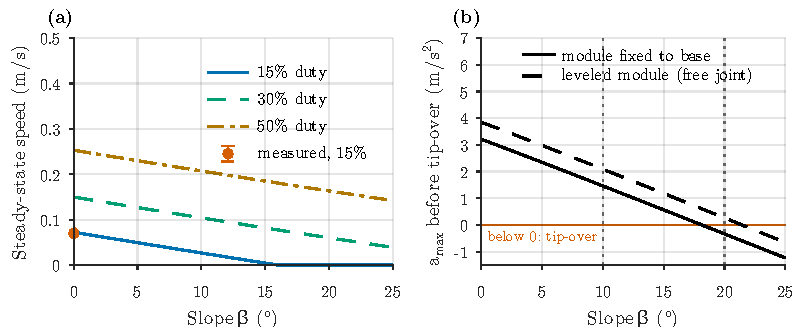
\includegraphics{figures/fig_base_limits.pdf}
  \caption{Mobile base. (a) Steady-state speed versus slope from \eqref{eq:vss} for three duty cycles, together with the measured speed at 15\% on flat ground. (b) Longitudinal acceleration margin before backward tip-over \eqref{eq:tip} with the module on the spherical joint, calibrated against the measured tip-over slope (dot).}
  \label{fig:base}
\end{figure}

\subsection{Aerial module dynamics}
\label{sec:aerial}

\paragraph{Rotor model and control allocation}
Each rotor produces thrust $F_i$ along $\vect z_D$ and reaction torque $-c_Qs_iF_i$ about $\vect z_D$, where $s_i=+1$ for counterclockwise rotors (viewed from above). Using the rotor positions $\vect r_i=[x_i,y_i,h_r]\T$ from Table~\ref{tab:params}, the collective thrust and body-frame torques are
\begin{equation}
  \begin{bmatrix}T\\ \tau_x\\ \tau_y\\ \tau_z\end{bmatrix}=\underbrace{\begin{bmatrix}\vect 1\T\\ \vect y\T\\ -\vect x\T\\ -c_Q\vect s\T\end{bmatrix}}_{\vect B\in\mathbb R^{4\times8}}\vect F,
  \qquad \vect B\vect B\T=\diag\big(8,\ 4L_r^2,\ 4L_r^2,\ 8c_Q^2\big),
  \label{eq:alloc}
\end{equation}
because $\sum x_i=\sum y_i=\sum s_i=\sum x_iy_i=\sum s_ix_i=\sum s_iy_i=0$ and $\sum x_i^2=\sum y_i^2=4L_r^2$ for the octocopter geometry (arm height $h_r$ does not contribute because thrust is parallel to $\vect z_D$). The four channels are therefore orthogonal, and the minimum-norm allocation is explicit:
\begin{equation}
  \vect F=\vect B\T(\vect B\vect B\T)^{-1}\vect w=\frac{T}{8}\vect 1+\frac{\vect y\,\tau_x-\vect x\,\tau_y}{4L_r^2}-\frac{\vect s\,\tau_z}{8c_Q},\qquad \vect w=[T,\tau_x,\tau_y,\tau_z]\T .
  \label{eq:alloc_inv}
\end{equation}
The firmware implements \eqref{eq:alloc_inv} directly \cite{johansen2013}: the collective sets the baseline force $F_0=T/8$, roll and pitch increments are added, and the yaw increment is added along the yaw row projected onto the null space of the other three rows (which, by the orthogonality above, is the yaw row itself). When an increment would drive any rotor outside $[F_{\min},F_{\max}]$ (\SIrange{1180}{2000}{\micro\second}), roll and pitch are scaled first and yaw second. For pure pitch torque, the $x$-axis rotors ($|x_i|=L_r$) saturate first, giving the achievable torque
\begin{equation}
  |\tau_y|_{\max}=4L_r\,\min\{F_{\max}-F_0,\ F_0-F_{\min}\},
  \label{eq:taumax}
\end{equation}
which, under the firmware thrust map, equals \SI{3.2}{\newton\metre} at a collective of \SI{1750}{\micro\second} and \SI{2.4}{\newton\metre} at \SI{1816}{\micro\second}---well above the torques required in hover (Section~\ref{sec:authority}). The firmware converts each force to a pulse width by inverting $F=k_F\big((u-u_0)/\SI{860}{\micro\second}\big)^n$ with $k_F=\SI{5.40}{\newton}$; if the true gain is $k_F'$, every torque generated by the controller is multiplied by the thrust-gain ratio $k_T=k_F'/k_F$, identified in Section~\ref{sec:ident}.

\paragraph{Newton--Euler equations about the moving pivot}
The rotating assembly (mass $m$, inertia $\vect J$ about the spherical joint, center of mass at $\vect r_c=[\delta_x,\delta_y,h_c]\T$ in $\{D\}$) rotates about the spherical joint center, a body-fixed point whose acceleration $\vect a_J$ \eqref{eq:aJ} is imposed by the base and vertical guide. For a body-fixed point on a rigid body, the angular momentum about it is $\vect J\vect\omega_D$, and its inertial derivative equals the external moment minus $m\,\vect r_c\times\vect a_J$ \cite{ginsberg1998}. In $\{D\}$ components:
\begin{equation}
  \vect J\dot{\vect\omega}_D+\vect\omega_D\times\vect J\vect\omega_D=
  \underbrace{\sum_{i=1}^{8}\vect r_i\times F_i\ez-\sum_{i=1}^{8}c_Qs_iF_i\ez}_{[\tau_x,\ \tau_y,\ \tau_z]\T}
  +\,m\,\vect r_c\times\Rot_{WD}\T\big(\vect g_W-\vect a_J\big)-\vect\tau_f ,
  \label{eq:euler}
\end{equation}
with $\vect g_W=[0,0,-g]\T$ and spherical-joint friction $\vect\tau_f$. The third term contains the three couplings that dominate module behavior. Linearizing about level hover (verified symbolically, \ref{app:derivations}):
\begin{align}
  J_x\ddot\phi&=\tau_x+m(g+a_{J,z})h_c\,\phi+m h_c\,a_{J,y}-m g\,\delta_y, \label{eq:rolllin}\\
  J_y\ddot\theta&=\tau_y+m(g+a_{J,z})h_c\,\theta-m h_c\,a_{J,x}+m g\,\delta_x, \label{eq:pitchlin}
\end{align}
with $\vect a_J$ in $\{D\}$ components. (i) Because $h_c>0$, the module is an inverted pendulum on the spherical joint, with open-loop poles $\pm p$, $p=\sqrt{mgh_c/J_y}=\SI{6.1}{\radian\per\second}$ for $h_c=\SI{0.14}{\metre}$ (doubling time \SI{0.11}{\second}). (ii) Horizontal base acceleration produces the torque $\mp mh_ca_J$: the top of the module lags behind the spherical joint, which is the primary disturbance path from the base to the octocopter. (iii) A horizontal CM eccentricity $\delta$ produces a constant torque $mg\delta$ that the controller must permanently oppose. Vertical spherical-joint acceleration parametrically modulates pendulum stiffness.

Along the vertical guide (axis $\vect z_B$), the carriage and module obey
\begin{equation}
  (m+m_c)\ddot d=T\,\vect z_D\!\cdot\!\vect z_B-(m+m_c)\big(g\cos\beta+\vect a_B\!\cdot\!\vect z_B\big)-F_g(\dot d)+F_{\mathrm{stop}},
  \label{eq:guide}
\end{equation}
so the module lifts off when $T>(m+m_c)g\cos\beta+F_{g,\mathrm{static}}$. While $T$ stays lower, the module rests on the lower stop and transmits its weight minus $T$ to the base; this is the weight relief exploited on the ramp (Section~\ref{sec:porquedron}).

\paragraph{Hover power}
By momentum theory \cite{leishman2006}, hover thrust per rotor, $T/8=\SI{4.41}{\newton}$, across a 9.4-inch propeller disk induces a velocity $v_h=\sqrt{T/(16\rho A)}=\SI{6.4}{\metre\per\second}$ and requires an ideal power of $Tv_h/8=\SI{28}{\watt}$ per rotor. With a figure of merit of 0.5 and a motor--ESC efficiency of 0.8, the eight rotors draw roughly \SI{570}{\watt}; the A2212 datasheet table with a 9450 propeller, scaled to \SI{3.6}{\kilo\gram}, gives \SI{500}{\watt}. That equals 22--\SI{25}{\ampere} per fused branch, and power grows as $T^{3/2}$, so every collective increase to offset voltage sag costs current. This is why the firmware limits operation above \SI{1850}{\micro\second} to \SI{20}{\second} (\SI{30}{\ampere} fuses), and why a \SI{29}{\milli\metre} propeller tip clearance was kept with $L_r=\SI{0.350}{\metre}$. Section~\ref{sec:bateria} translates these figures into thrust margin and endurance.

\subsection{Aerial module identification from hover telemetry}
\label{sec:ident}

\paragraph{Thrust gain}
At liftoff, \eqref{eq:guide} gives $8k_F'\big((u-u_0)/860\big)^n=(m+m_c)g+F_{g,\mathrm{static}}$. Liftoff occurred between \SI{1725}{\micro\second} and \SI{1775}{\micro\second} with charged LiPo packs at 12.4\,V at rest at the start of the session (Section~\ref{sec:flights}); neglecting guide friction yields lower bounds $k_F'=$ \SIrange{7.17}{8.18}{\newton}, so the thrust-gain ratio is $k_T=1.33$--1.52 (Fig.~\ref{fig:ident}b). The firmware map, and the Isaac Lab model built on it, predicted hover at \SI{1899}{\micro\second}; an independent power audit based on motor and propeller data predicted \SI{1770}{\micro\second}, inside the measured band, though for a mass of \SI{3.10}{\kilo\gram} rather than \SI{3.6}{\kilo\gram}.

\paragraph{Center of mass}
During quasi-static hover ($\dot{\vect\omega}_D\approx\vect 0$, integrators settled, $T\approx(m+m_c)g$), \eqref{eq:rolllin}--\eqref{eq:pitchlin} reduce to moment balances. Dividing by collective thrust cancels the unknown gain $k_F'$ and leaves the center-of-thrust coordinates,
\begin{equation}
  x_{cp}=\frac{\sum_i x_iF_i}{\sum_iF_i}=c\,(\delta_x+h_c\sin\theta),\qquad
  y_{cp}=\frac{\sum_i y_iF_i}{\sum_iF_i}=c\,(\delta_y-h_c\sin\phi),
  \label{eq:cop}
\end{equation}
with $c=m/(m+m_c)$, which is linear in $(\delta_x,\delta_y,h_c)$ and computed from logged motor commands. Averaging \eqref{eq:cop} over the hover phase of the seven flights that lifted off (samples with $|p|,|q|<\SI{15}{\degree\per\second}$ above \SI{1650}{\micro\second}) and solving the 14 equations by least squares gives
\begin{equation}
  \hat\delta_x=9.5\pm1.8\ \mathrm{mm},\qquad \hat\delta_y=1.9\pm1.5\ \mathrm{mm},\qquad \hat h_c=0.14\pm0.06\ \mathrm{m}\quad(\pm1\sigma),
  \label{eq:idres}
\end{equation}
with an RMS residual of \SI{3.3}{\milli\metre} (Fig.~\ref{fig:ident}a). The estimate of $h_c$ shifts by less than its uncertainty when the map exponent varies between 1.3 and 1.6 (0.11--\SI{0.14}{\metre}), and agrees with the \SI{0.10}{\metre} value from the CAD model. The eccentricity produces a constant gravity torque $mg\delta_x=\SI{0.31}{\newton\metre}$ toward M8.

\begin{figure}[!htbp]
  \centering
  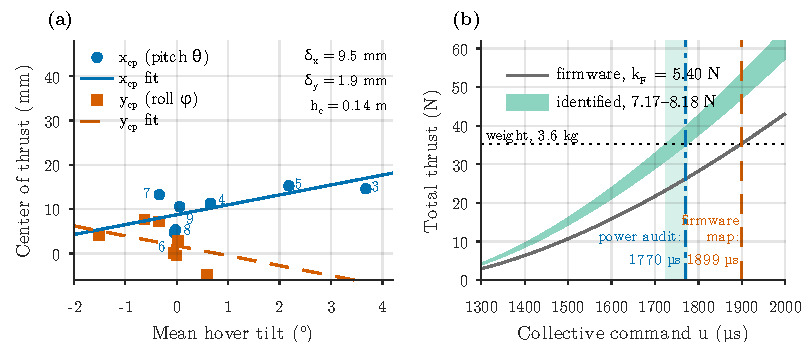
\includegraphics{figures/fig_ident.pdf}
  \caption{Identification from hover telemetry. (a) Center of thrust versus mean tilt across the seven hover flights (labels: flight number) and least-squares fit of \eqref{eq:cop}. (b) Total thrust from the firmware map, band identified from the liftoff condition, moving-assembly weight, and hover predictions from the firmware map and power audit.}
  \label{fig:ident}
\end{figure}

\subsection{Ball on an accelerating and rotating plate}
\label{sec:ball}

Let $\vect\Omega$ be the angular velocity of the plate frame $\{P\}$ and let $\vect a_G$ be the absolute acceleration of its origin (the universal joint center), both expressed in $\{P\}$. The ball center is at $\vect\rho=[x_b,y_b,\varepsilon]\T$, its absolute angular velocity is $\vect\omega_b$, and rolling without slip (A6) requires the contact-point velocity of the ball to equal that of the plate surface beneath it. This gives $\dot{\vect\rho}=r_b(\vect\omega_b-\vect\Omega)\times\ez$, i.e., the relative angular velocity is $\vect w=\vect\omega_b-\vect\Omega=[-\dot y_b/r_b,\ \dot x_b/r_b,\ w_z]\T$, with a free spin $w_z$ about the plate normal. Writing Newton's law for the ball center in the rotating frame and Euler's law for the ball about its center, with the contact force applied at $-r_b\ez$, and eliminating the tangential contact forces (\ref{app:derivations}) yields, exactly,
\begin{align}
  \frac{\ddot x_b}{\gamma_b}&=g_x-a_{G,x}-\kappa\dot\Omega_y+\dot\Omega_z\,y_b+(\Omega_y^2+\Omega_z^2)\,x_b-\Omega_x\Omega_y\,y_b \notag\\
   &\quad-\varepsilon\,\Omega_x\Omega_z+(2+\iota)\,\Omega_z\dot y_b+\iota r_b\,\Omega_xw_z, \label{eq:ballx}\\
  \frac{\ddot y_b}{\gamma_b}&=g_y-a_{G,y}+\kappa\dot\Omega_x-\dot\Omega_z\,x_b+(\Omega_x^2+\Omega_z^2)\,y_b-\Omega_x\Omega_y\,x_b \notag\\
   &\quad-\varepsilon\,\Omega_y\Omega_z-(2+\iota)\,\Omega_z\dot x_b+\iota r_b\,\Omega_yw_z, \label{eq:bally}\\
  \dot w_z&=-\dot\Omega_z-\frac{\Omega_x\dot x_b+\Omega_y\dot y_b}{r_b}, \label{eq:spin}
\end{align}
where $[g_x,g_y,g_z]\T=\Rot_{WP}\T\vect g_W$ is gravity in $\{P\}$, $\iota=I_b/(m_br_b^2)$ ($2/5$ for a solid sphere), $\gamma_b=1/(1+\iota)$, and
\begin{equation}
  \kappa=\varepsilon+\frac{I_b}{m_br_b}=\varepsilon+\iota r_b=\SI{42.3}{\milli\metre}
  \label{eq:kappa}
\end{equation}
is the effective height of the ball above the rotation axis. Equations \eqref{eq:ballx}--\eqref{eq:spin} contain the classical ball-and-plate model as the special case $\vect a_G=\vect 0$, $\Omega_z=0$, $\varepsilon=0$ \cite{awtar2002,hauser1992}; the additional terms are the translational acceleration of the plate center, the Euler term $\kappa\dot{\vect\Omega}$ from ball height, centrifugal and Coriolis terms from base rotation, and spin coupling.

\paragraph{Linearization and transfer functions}
For small angles, $g_x\simeq g\,\Theta_P$ and $g_y\simeq-g\,\Phi_P$; with \eqref{eq:tilt} and the linearization of \eqref{eq:aG}, $a_{G,x}\simeq a_{J,x}+h_P\ddot\theta$ and $a_{G,y}\simeq a_{J,y}-h_P\ddot\phi$, the ball obeys
\begin{align}
  \ddot x_b&=\gamma_b\Big[g(\theta+\alpha_y)-\kappa\,\ddot\alpha_y-(h_P+\kappa)\,\ddot\theta-a_{J,x}\Big], \label{eq:balllinx}\\
  \ddot y_b&=\gamma_b\Big[-g(\phi+\alpha_x)+\kappa\,\ddot\alpha_x+(h_P+\kappa)\,\ddot\phi-a_{J,y}\Big]. \label{eq:balllinly}
\end{align}
Equations \eqref{eq:balllinx}--\eqref{eq:balllinly} summarize the coupling across the entire robot: the ball is driven by servo tilt (the control input), residual octocopter attitude amplified by the lever arm $h_P+\kappa=\SI{0.146}{\metre}$, and spherical-joint acceleration produced by the base. With $\alpha_y=K_\alpha u$, the three $x$-axis transfer functions are
\begin{equation}
  \frac{X_b}{U}=K_b\,\frac{1-s^2/z_1^2}{s^2},\qquad
  \frac{X_b}{\Theta}=\gamma_b g\,\frac{1-s^2/z_2^2}{s^2},\qquad
  \frac{X_b}{A_{J,x}}=-\frac{\gamma_b}{s^2},
  \label{eq:balltf}
\end{equation}
with plant gain $K_b=\gamma_bgK_\alpha=\SI{6.0}{\milli\metre\per\second\squared}$ per microsecond (solid sphere) and zeros $z_1=\sqrt{g/\kappa}=\SI{15.2}{\radian\per\second}$ and $z_2=\sqrt{g/(h_P+\kappa)}=\SI{8.2}{\radian\per\second}$. Each pair contains a right-half-plane zero: the servo path is non-minimum phase (a rapid tilt initially pushes the ball in the wrong direction because the plate surface accelerates beneath it), and above $z_2/2\pi=\SI{1.3}{\hertz}$ octocopter angular acceleration disturbs the ball more than its tilt.

\paragraph{Base rotation}
For a base turning at constant rate $\omega$ ($\vect\Omega=\omega\ez$), \eqref{eq:ballx}--\eqref{eq:bally} add negative stiffness $\gamma_b\omega^2$ and gyroscopic coupling $\gamma_b(2+\iota)\omega$ between axes. Even for a turn faster than any test ($\omega=\SI{0.53}{\radian\per\second}$, wheels at $\pm\SI{0.10}{\metre\per\second}$), the negative stiffness is \SI{0.20}{\per\second\squared}, less than 10\% of the stiffness $K_bk_p\approx\SI{2}{\per\second\squared}$ provided by the ball controller (Section~\ref{sec:ballcontrol}).
           % 3. Model: base, octocopter, and ball dynamics
%% ======================================================================
%% 04d_dron_rampa_bateria.tex -- 3. Model (part 3): why a drone on the ramp and battery margin
%% Numbers: scripts_modelo/rampa.py and scripts_modelo/bateria.py
%% ======================================================================
\subsection{Why a drone on the ramp}
\label{sec:porquedron}

AeroTray's intermediate stage could have been a motorized two-axis gimbal. Using the equations derived above, this section quantifies what the octocopter contributes on the ramp and at what cost.

\paragraph{Core idea: an actuator that does not push against the base}
A plate driven by base-mounted servos, or by a motorized gimbal, generates its torque \emph{between} the base and the plate. By action and reaction, three things happen: every base tilt (both the slope and the jolts across the ramp breaks) must be subtracted out of the actuator's own stroke; those jolts reach the plate through a rigid transmission; and the level reference is the base itself. The octocopter on the spherical joint breaks that chain. The spherical joint transmits force only, not torque. The drone generates its torque against the air and references gravity with its IMU. Ground slope therefore never enters the plate, and the actuators separate by scale: the drone handles large, slow angles (the slope, \SIrange{0}{20}{\degree}, below \SI{0.3}{\hertz}), while the servos handle the small, fast angles required by the ball. No stage reacting against the base can provide this separation without consuming actuator stroke. The drone also adds an exclusive capability: its thrust acts as adjustable ballast (point~2).

\paragraph{Evidence from the 18 November logs}
Across the eleven runs recorded that day, the drone sat free on the spherical joint at \SI{1300}{\micro\second}. Mean servo stroke usage was 36--57\% over the seven ramp runs and 43--63\% over the four flat-ground runs. Median pulse-width bias on the ramp never exceeded \SI{\pm60}{\micro\second}. With the tray fixed to the base, merely leveling the \SI{10}{\degree} slope would have required a bias of about \SI{204}{\micro\second}---93\% of available stroke. The servos worked no harder on the ramp than on flat ground: the slope did not reach the plate. A direct comparative test---Test~D in Section~\ref{sec:metodologia}, traversing the same ramp with the drone locked to the base (\emph{servos only}) versus free on the joint to compare servo usage, saturation, ball error, and losses---remains future work (Section~\ref{sec:limits}).

\paragraph{1. Leveling: slope disappears from the plate}
By \eqref{eq:tilt}, absolute plate tilt is $\theta+\alpha_y$ and does not contain $\beta$. The octocopter drives $\theta$ to zero using its own IMU, so the servos only regulate ball position. With the tray fixed to the base, the slope would consume $\beta$ of the \SI{\pm10.8}{\degree} plate travel: on the \SI{10}{\degree} ramp only \SI{0.8}{\degree} would remain for ball control, and at \SI{20}{\degree} the plate could not level. In hover, the octocopter held the tray plane within 0.55--1.7$^\circ$ RMS of horizontal (Section~\ref{sec:flights}), leaving 84--95\% of the servo stroke free. A gimbal with its own IMU could also level the tray, though still reacting against the base with finite actuator stroke; the next function, however, is exclusive to the drone.

\paragraph{2. Weight relief: adjustable ballast}
Let $f=T/\big((m+m_c)g\big)\in[0,1]$ be the fraction of the module weight supported by the rotors. While $f<1$, the module rests on the lower stop of the vertical guide \eqref{eq:guide}, and because it self-levels, its thrust is vertical in $\{W\}$. In the moment balance \eqref{eq:tip}, thrust therefore reduces the effective weight of the module at the spherical joint to $(1-f)(m+m_c)$. With the rest of the robot (mass $M_b=\SI{6.8}{\kilo\gram}$, CM at $x_b=\SI{0.088}{\metre}$ ahead of the driven axle and $h_b=\SI{0.081}{\metre}$ above the support plane, deduced from the measured tip-over slopes) and $m_a=m+m_c$,
\begin{equation}
\begin{gathered}
  M(f)=M_b+(1-f)m_a,\\
  x_G(f)=\frac{M_bx_b+(1-f)m_a\ell_J}{M(f)},\qquad
  h_G(f)=\frac{M_bh_b+(1-f)m_a(h_{J0}+d)}{M(f)},
\end{gathered}
  \label{eq:descarga}
\end{equation}
and substituting \eqref{eq:descarga} into the static condition of \eqref{eq:tip}, \eqref{eq:vss}, and the traction condition of Section~\ref{sec:basedyn} gives the relieved limits. The acceleration margin requires one extra distinction: thrust removes \emph{weight}, not \emph{mass}. The vertical guide still accelerates all \SI{3.6}{\kilo\gram} of the module together with the base, so its full d'Alembert force acts at the spherical joint and
\begin{equation}
\begin{split}
  a_{\max}(f,\beta)=\frac{g}{M_bh_b+m_a(h_{J0}+d)}\Big\{&\big[M_bx_b+(1-f)m_a\ell_J\big]\cos\beta\\
  &-\big[M_bh_b+(1-f)m_a(h_{J0}+d)\big]\sin\beta\Big\}.
\end{split}
  \label{eq:amaxf}
\end{equation} Figure~\ref{fig:rampa} and Table~\ref{tab:rampa} show the outcome. The \SI{3.6}{\kilo\gram} module sits high (spherical joint at \SI{0.5}{\metre}) and nearly on the same vertical line as the CM of the rest of the robot ($\ell_J\approx x_b\approx\SI{88}{\milli\metre}$). Supporting a fraction $f$ of its weight with the rotors therefore shifts the CM neither forward nor backward: it \emph{lowers} it, improving tip-over stability in both directions.
\begin{itemize}
  \item \textbf{Tip-over.} Uphill static tip-over slope rises from \SI{21.4}{\degree} ($f=0$; measured: \SI{21.5}{\degree}) to \SI{27.7}{\degree} ($f=0.5$) and \SI{47.4}{\degree} ($f=1$). Downhill, it rises from \SI{30.5}{\degree} to \SI{38.2}{\degree} and \SI{58.5}{\degree}. On the \SI{10}{\degree} ramp, the uphill margin grows from \SI{11.5}{\degree} to \SI{17.7}{\degree} at $f=0.5$, a 54\% increase.
  \item \textbf{Acceleration margin.} At \SI{10}{\degree} it barely changes (\SI{2.1}{\metre\per\second\squared}), because thrust removes weight rather than mass \eqref{eq:amaxf}. At \SI{20}{\degree} it grows from \SI{0.26}{\metre\per\second\squared} to \SI{0.92}{\metre\per\second\squared} at $f=0.5$---a 3.5-fold increase. Weight relief becomes decisive on steep slopes.
  \item \textbf{Traction.} The friction coefficient required at the driven wheels increases modestly: from 0.25 to 0.27 at \SI{10}{\degree} and from 0.40 to 0.44 at \SI{20}{\degree} for $f=0.5$, reaching 0.52 at $f=1$. All values stay below the rubber-on-wood range (0.5--0.8). Even so, the drone should not hover on the ramp: at $f=1$, traction on a \SI{20}{\degree} slope sits at the limit.
\end{itemize}
We propose an operating window of $f=0.35$--0.55 (\emph{ramp mode}). This corresponds to a collective of 1460--\SI{1560}{\micro\second} on charged batteries---below the firmware flight threshold (\SI{1650}{\micro\second})---and 5--\SI{9}{\ampere} per branch (power scales as $f^{3/2}$). One minute of climbing draws 0.08--\SI{0.15}{\ampere\hour} per battery, or 2--5\% of capacity. On the actual test ramp (\SI{0.7}{\metre} uphill at \SI{10}{\degree}, \SI{0.8}{\metre} flat plateau, and \SI{0.7}{\metre} downhill, \SI{12.2}{\centi\metre} height; Fig.~\ref{fig:rampa_cotas}), the model predicts a full cycle at 15\% duty cycle of about \SI{41}{\second} at idle (\SI{24}{\second} climb) and \SI{37}{\second} in ramp mode (\SI{20}{\second} climb), and about \SI{19}{\second} at 25\% duty cycle (23 November tests).

\begin{figure}[!htbp]
\centering
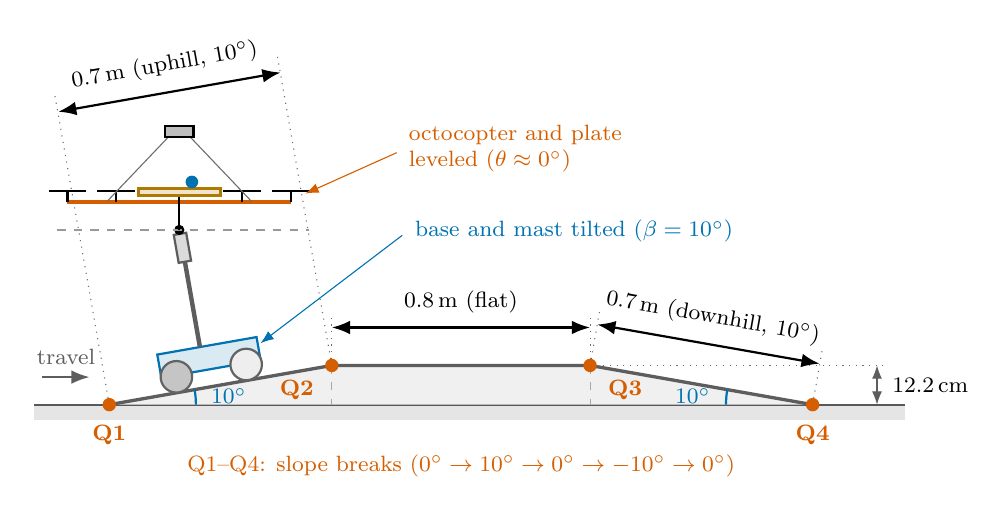
\begin{tikzpicture}[font=\footnotesize, >=Latex]
  % True scale (1 m = 4.10 cm). Ramp measured 24 Nov: 0.7 m at 10 deg + 0.8 m + 0.7 m at 10 deg
  % Q1=(0,0), Q2=(2.826, 0.498), Q3=(6.106, 0.498), Q4=(8.932, 0)
  \coordinate (Q1) at (0.000, 0.000);
  \coordinate (Q2) at (2.826, 0.498);
  \coordinate (Q3) at (6.106, 0.498);
  \coordinate (Q4) at (8.932, 0.000);

  % Level ground (approach and exit)
  \fill[pGris!18] (-0.95,-0.20) rectangle (10.10,0.00);
  \draw[thick, pGris!80!black] (-0.95,0.00) -- (10.10,0.00);

  % Ramp profile (1:1 scale)
  \fill[pGris!10] (Q1) -- (Q2) -- (Q3) -- (Q4) -- cycle;
  \draw[very thick, pGris!85!black] (Q1) -- (Q2) -- (Q3) -- (Q4);

  % Subtle vertical dashed guides under plateau
  \draw[dashed, pGris!60] (Q2) -- (2.826,0.00);
  \draw[dashed, pGris!60] (Q3) -- (6.106,0.00);

  % 10 deg slope angles at Q1 and Q4
  \draw[pAzul, thick] (1.10,0.00) arc (0:10:1.10);
  \node[pAzul] at (1.52,0.11) {\SI{10}{\degree}};
  \draw[pAzul, thick] (7.832,0.00) arc (180:170:1.10);
  \node[pAzul] at (7.41,0.11) {\SI{10}{\degree}};

  % Vertical height dimension (12.2 cm) on the right
  \draw[dotted, pGris] (Q3) -- (9.90,0.498);
  \draw[<->, pGris!85!black] (9.75,0.00) -- (9.75,0.498);
  \node[right=2pt, align=left] at (9.75,0.25) {\SI{12.2}{\centi\metre}};

  % Schematic robot climbing the ramp (1:1 true proportions, centered at s=0.47 m)
  \begin{scope}[shift={(1.330,0.235)}, rotate=10]
    % Differential base chassis + wheels (wheelbase L=0.22 m -> 0.90 cm, r=0.049 m -> 0.20 cm)
    \draw[thick, fill=pAzul!15, draw=pAzul] (-0.64,0.22) rectangle (0.64,0.52);
    \draw[thick, fill=pGris!40, draw=pGris!90!black] (-0.45,0.20) circle (0.20);
    \draw[thick, fill=pGris!12, draw=pGris!90!black] ( 0.45,0.20) circle (0.20);
    % Mast and vertical guide carriage (l_J=0.088 m -> 0.36 cm ahead of driven axle)
    \draw[line width=1.6pt, pGris!85!black] (-0.09,0.52) -- (-0.09,1.98);
    \draw[thick, fill=pGris!25, draw=pGris!85!black] (-0.17,1.62) rectangle (-0.01,1.98);
    \coordinate (J) at (-0.09,2.03);
    \coordinate (BaseTip) at (0.64,0.40);
  \end{scope}

  % Leveled octocopter and tray (theta = 0 deg) on spherical joint J
  \fill[black] (J) circle (0.065);
  \begin{scope}[shift={(J)}]
    % Horizontal reference through spherical joint
    \draw[dashed, pGris!70] (-1.55,0.00) -- (1.65,0.00);
    % Red octocopter frame (2 L_r = 0.70 m -> 2.87 cm)
    \draw[line width=1.4pt, pRojo] (-1.42,0.36) -- (1.42,0.36);
    \foreach \xx in {-1.42,-0.80,0.80,1.42}{
      \draw[thick] (\xx,0.36) -- (\xx,0.49);
      \draw[thick] (\xx-0.24,0.49) -- (\xx+0.24,0.49);
    }
    % Pillar, plate (ochre), and ball (blue)
    \draw[thick] (0,0.00) -- (0,0.44);
    \draw[very thick, pOcre, fill=pOcre!20] (-0.52,0.44) rectangle (0.52,0.53);
    \fill[pAzul] (0.16,0.61) circle (0.08);
    % Camera towers and overhead camera
    \draw[thin, pGris] (-0.92,0.36) -- (-0.12,1.20);
    \draw[thin, pGris] ( 0.92,0.36) -- ( 0.12,1.20);
    \draw[thick, fill=pGris!45] (-0.18,1.18) rectangle (0.18,1.32);
    \coordinate (OctoR) at (1.50,0.40);
  \end{scope}

  % Clean robot annotations (in open space on the right, clear of flat-segment dimension)
  \draw[->, pRojo, thin] (3.65,3.20) -- (2.49,2.68);
  \node[pRojo, right, align=left] at (3.68,3.25) {octocopter and plate\\ leveled ($\theta\approx\SI{0}{\degree}$)};
  \draw[->, pAzul, thin] (3.72,2.15) -- (1.92,0.78);
  \node[pAzul, right, align=left] at (3.76,2.20) {base and mast tilted ($\beta=\SI{10}{\degree}$)};

  % Parallel dimensions for the three ramp segments
  % Segment 1: uphill 0.7 m (above robot, with extension lines from Q1 and Q2)
  \coordinate (Q1u) at ($(Q1)+(-0.69,3.92)$);
  \coordinate (Q2u) at ($(Q2)+(-0.69,3.92)$);
  \draw[dotted, pGris] (Q1) -- (Q1u);
  \draw[dotted, pGris] (Q2) -- (Q2u);
  \draw[<->, thick] ($(Q1)+(-0.65,3.72)$) -- node[above=2pt, sloped]{\SI{0.7}{\metre} (uphill, \SI{10}{\degree})} ($(Q2)+(-0.65,3.72)$);

  % Segment 2: flat plateau 0.8 m (lowered to y=0.98 to clear the blue arrow)
  \draw[dotted, pGris] (Q2) -- (2.826,1.12);
  \draw[dotted, pGris] (Q3) -- (6.106,1.12);
  \draw[<->, thick] (2.826,0.98) -- node[above=1.5pt]{\SI{0.8}{\metre} (flat)} (6.106,0.98);

  % Segment 3: downhill 0.7 m
  \coordinate (Q3d) at ($(Q3)+(0.13,0.74)$);
  \coordinate (Q4d) at ($(Q4)+(0.13,0.74)$);
  \draw[dotted, pGris] (Q3) -- (Q3d);
  \draw[dotted, pGris] (Q4) -- (Q4d);
  \draw[<->, thick] ($(Q3)+(0.09,0.52)$) -- node[above=2pt, sloped]{\SI{0.7}{\metre} (downhill, \SI{10}{\degree})} ($(Q4)+(0.09,0.52)$);

  % Markers for the 4 slope breaks (Q1..Q4)
  \foreach \q in {Q1, Q2, Q3, Q4}{
    \fill[pRojo] (\q) circle (0.085);
  }
  \node[pRojo, font=\footnotesize\bfseries, below=4pt] at (Q1) {Q1};
  \node[pRojo, font=\footnotesize\bfseries, below left=2pt and 3pt] at (Q2) {Q2};
  \node[pRojo, font=\footnotesize\bfseries, below right=2pt and 3pt] at (Q3) {Q3};
  \node[pRojo, font=\footnotesize\bfseries, below=4pt] at (Q4) {Q4};

  % Travel direction and slope-break note below ground (clear of Q1 and Q4)
  \draw[->, thick, pGris!85!black] (-0.85,0.35) -- (-0.25,0.35);
  \node[above=1pt, pGris!85!black] at (-0.55,0.35) {travel};
  \node[pRojo] at (4.47,-0.78) {Q1--Q4: slope breaks ($0^\circ \to 10^\circ \to 0^\circ \to -10^\circ \to 0^\circ$)};
\end{tikzpicture}
\caption{Geometry of the test ramp, to scale (measured: \SI{0.7}{\metre} uphill at \SI{10}{\degree}, \SI{0.8}{\metre} flat plateau, and \SI{0.7}{\metre} downhill at \SI{10}{\degree}; \SI{12.2}{\centi\metre} height, \SI{2.18}{\metre} horizontal length) with AeroTray in true proportion. Points Q1--Q4 mark the four slope breaks where base pitch changes and the spherical joint receives tangential accelerations $(h_{J0}+d)\ddot\theta_B$; during the climb, the octocopter stays horizontal on the passive spherical joint.}
\label{fig:rampa_cotas}
\end{figure}

\begin{table}[!htbp]
\centering
\caption{Effect of the module weight fraction supported by the rotors, $f$, on climbing performance (model \eqref{eq:descarga}--\eqref{eq:amaxf} with parameters from Table~\ref{tab:params}; $k_F'=\SI{7.6}{\newton}$, charged LiPo packs). At idle (\SI{1300}{\micro\second}), the rotors already support 12\% of the weight.}
\label{tab:rampa}
\resizebox{\textwidth}{!}{%
\begin{tabular}{@{}lccccccc@{}}
\toprule
$f$ & Uphill tip-over & Downhill tip-over & $a_{\max}$ at \SI{20}{\degree} & Req.\ $\mu$ \SI{10}{\degree} & Req.\ $\mu$ \SI{20}{\degree} & Collective & $I$ per branch \\
 & (\si{\degree}) & (\si{\degree}) & (\si{\metre\per\second\squared}) & & & (\si{\micro\second}) & (\si{\ampere}) \\
\midrule
0 (motors off) & 21.4 (measured 21.5) & 30.5 (measured 30.5) & 0.26 & 0.25 & 0.40 & $\le$1140 & 0 \\
0.12 (idle) & 22.5 & 31.9 & 0.42 & 0.25 & 0.40 & 1300 & 0.9 \\
0.25 & 23.9 & 33.6 & 0.59 & 0.26 & 0.41 & 1397 & 2.8 \\
0.50 & 27.7 & 38.2 & 0.92 & 0.27 & 0.44 & 1537 & 7.9 \\
0.75 & 34.2 & 45.6 & 1.25 & 0.28 & 0.47 & 1652 & 14.5 \\
1 & 47.4 & 58.5 & 1.57 & 0.30 & 0.52 & 1752 & 22.3 \\
\bottomrule
\end{tabular}}
\end{table}

\begin{figure}[!htbp]
  \centering
  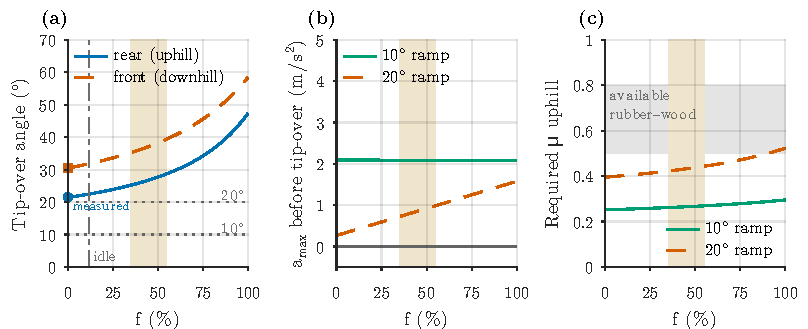
\includegraphics{figures/fig_rampa.pdf}
  \caption{Weight relief on the ramp versus the module weight fraction supported by the rotors, $f$ ($f=0.5$ corresponds to about \SI{1540}{\micro\second} collective). (a) Static backward (uphill forward) and forward (downhill forward) tip-over slopes; dots show the slopes measured on 23 November with the module locked. (b) Tip-over-free acceleration margin at \SI{10}{\degree} and \SI{20}{\degree}, with the full module inertia \eqref{eq:amaxf}. (c) Friction coefficient required at the driven wheels while climbing, with the rubber-on-wood band. The ochre band marks the proposed ramp-mode window.}
  \label{fig:rampa}
\end{figure}

\paragraph{3. Trade-off versus a gimbal}
An honest comparison with a lightweight gimbal is as follows. Under the same model, a \SI{1}{\kilo\gram} motorized gimbal at the same height would achieve a \SI{33.3}{\degree} uphill tip-over slope at zero power cost; the octocopter surpasses it only for $f>0.72$. The drone's advantage is therefore not low mass, but \emph{adjustable} ballast: at $f=0$ it loads the driven wheels for traction, at $f\approx0.5$ it balances tip-over and traction, and at $f=1$ its weight disappears from the base. A gimbal is fixed ballast. Moreover, the octocopter is the project's object of study: an inverted pendulum with actuator delay and limited torque authority validated here, captive and instrumented, prior to free flight. The cost is twofold: power (Section~\ref{sec:bateria}) and a 0.2--\SI{0.3}{\hertz} band in which the octocopter amplifies base accelerations (Section~\ref{sec:coupling}), which base reference ramps must avoid.

\paragraph{What was tested and what remains}
The \SI{10}{\degree} ramp runs on 18 November used the bench firmware with collective at \SI{1300}{\micro\second} ($f\approx0.12$): the drone leveled the tray while providing minimal weight relief. Weight relief is thus still a model prediction. Validating it requires three measurements: base motor current via clamp meter, the duty cycle required to climb at constant speed at $f=0$ and $f=0.5$, and the angle at which the omnidirectional wheels begin to lift on a variable-slope ramp.

\subsection{Thrust margin and endurance versus battery voltage}
\label{sec:bateria}

On 20 November, the module lifted off with the LiPo packs at 12.4\,V at rest, and later failed to lift off at 11.1\,V. This section explains that observation and calculates thrust margin and endurance.

\paragraph{Model}
Each ESC applies a fraction of its branch voltage, $V_{\mathrm{bus}}$, to the motor. With the propeller as load, rotor speed scales with voltage and thrust with its square, so at a fixed command,
\begin{equation}
  T=8k_F'\Big(\frac{V_{\mathrm{bus}}}{V_{\mathrm{ref}}}\Big)^2\Big(\frac{u-u_0}{860}\Big)^n ,
  \label{eq:tv}
\end{equation}
where $k_F'$ is the gain identified at voltage $V_{\mathrm{ref}}$ in Section~\ref{sec:ident}. The branch voltage equals the LiPo open-circuit voltage, $V_{oc}$, minus the drop across internal resistance, the \SI{1}{\metre} cable, and contacts (fuse, relay, XT60), $R_\Sigma$. Because hover power $P_b$ per branch is fixed (thrust equals weight), branch current is $I_b=P_b/V_{\mathrm{bus}}$, and
\begin{equation}
  V_{\mathrm{bus}}=\tfrac12\Big(V_{oc}+\sqrt{V_{oc}^2-4R_\Sigma P_b}\Big).
  \label{eq:vbus}
\end{equation}
Equating \eqref{eq:tv} to weight gives the liftoff collective at another voltage:
\begin{equation}
  u_{\mathrm{req}}=u_0+860\,x_{\mathrm{ref}}\Big(\frac{V_{\mathrm{bus,ref}}}{V_{\mathrm{bus}}}\Big)^{2/n},\qquad x_{\mathrm{ref}}=\frac{u_{\mathrm{ref}}-u_0}{860}=0.68\text{--}0.74,
  \label{eq:ureq}
\end{equation}
and with $n=1.6$ the collective grows as the $1.25$ power of the relative voltage drop. Inputs are: $P_b=\SI{250}{\watt}$ (A2212 with 9450 propeller table from the power audit, \SI{4.2}{\ampere} at 370\,gf and 11.1\,V, scaled as $T^{3/2}$ to 441\,gf per motor); $R_\Sigma=3r_c+\SI{22.6}{\milli\ohm}$, with $r_c=6$--\SI{15}{\milli\ohm} per cell [E] and a 50\% increase below 40\% state of charge; and a typical LiPo rest-voltage versus state-of-charge curve [E]. Result bands combine the extreme values of $k_F'$ and $r_c$.

\paragraph{Results}
Figure~\ref{fig:bateria} and Table~\ref{tab:bateria} give the liftoff collective and available thrust-to-weight ratio versus rest voltage:
\begin{itemize}
  \item At 12.4\,V (93\% charge), each branch delivers \SI{22}{\ampere} at \SI{11.2}{\volt}. The module lifts off at 1725--\SI{1775}{\micro\second}: the firmware \texttt{flotar} (hover) command (\SI{1750}{\micro\second}) falls squarely inside this band. At the \SI{1850}{\micro\second} sustained limit, the thrust-to-weight ratio is 1.20--1.36, and at the \SI{1950}{\micro\second} maximum, 1.48--1.68.
  \item At 11.1\,V at rest (12\% charge), bus voltage drops to \SI{9.3}{\volt} at \SI{27}{\ampere}, and liftoff demands 1850--\SI{2000}{\micro\second}: in the best case right at the sustained limit with no margin for attitude control, and in the worst case beyond what the ESC can deliver. This matches the experimental observation.
  \item The minimum rest voltage for liftoff without exceeding \SI{1850}{\micro\second} is 11.1--\SI{11.6}{\volt} (12--60\% charge). With the fixed \texttt{flotar} command, the module lifts off only above 12.05--\SI{12.1}{\volt}, and at the pessimistic bound of $k_F'$ it never lifts off.
  \item \textbf{Endurance.} Starting from 12.4\,V, continuous hover lasts 2.7--\SI{6.8}{\minute} until liftoff requires \SI{1850}{\micro\second} (3.3--\SI{7.4}{\minute} from 12.6\,V). The energy limit at 80\% discharge would be \SI{6.6}{\minute}. Flight time is therefore limited by thrust margin rather than battery capacity: only the upper end of the discharge curve is usable.
\end{itemize}

\begin{table}[!htbp]
\centering
\caption{Thrust margin versus LiPo voltage at rest (model \eqref{eq:vbus}--\eqref{eq:ureq}). Nominal collective computed with $u_{\mathrm{ref}}=\SI{1750}{\micro\second}$ and $r_c=\SI{10}{\milli\ohm}$; uncertainty band in parentheses.}
\label{tab:bateria}
\footnotesize
\setlength{\tabcolsep}{4pt}
\begin{tabular}{@{}cccccc@{}}
\toprule
$V_{oc}$ (V) & Charge (\%) & $V_{\mathrm{bus}}$ (V) & $I_b$ (A) & $u_{\mathrm{req}}$ (\si{\micro\second}) & Thrust/weight at \SI{1850}{\micro\second} \\
\midrule
12.6 & 100 & 11.45 & 21.8 & 1735 (1710--1760) & 1.24--1.42 \\
12.4 & 93 & 11.23 & 22.3 & 1750 (1725--1775) & 1.20--1.36 \\
12.2 & 84 & 11.00 & 22.7 & 1766 (1739--1793) & 1.14--1.31 \\
12.0 & 78 & 10.78 & 23.2 & 1782 (1754--1811) & 1.09--1.26 \\
11.8 & 68 & 10.55 & 23.7 & 1799 (1769--1831) & 1.04--1.21 \\
11.6 & 59 & 10.33 & 24.2 & 1817 (1786--1852) & 1.00--1.16 \\
11.4 & 40 & 10.10 & 24.8 & 1837 (1803--1875) & 0.95--1.12 \\
11.1 & 12 & 9.32 & 26.8 & 1910 (1850--2000) & 0.74--1.00 \\
\bottomrule
\end{tabular}
\end{table}

\begin{figure}[!htbp]
  \centering
  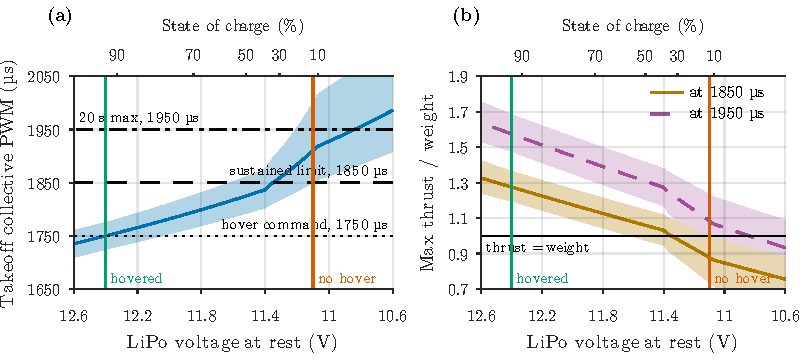
\includegraphics{figures/fig_bateria.pdf}
  \caption{Thrust margin versus LiPo voltage at rest. (a) Liftoff collective \eqref{eq:ureq}: nominal curve and band from uncertainty in $k_F'$ and internal resistance; horizontal lines show the \texttt{flotar} command, sustained limit, and maximum command of firmware v11; top axis shows state of charge. (b) Available thrust-to-weight ratio at the sustained limit and at maximum collective.}
  \label{fig:bateria}
\end{figure}

\paragraph{Comparison with flight logs}
Integrating the logged motor commands from Flights~6--9 on 20 November with the same power model gives a charge draw per battery of 0.10, 0.22, 0.25, and \SI{0.44}{\ampere\hour} (\SI{1.0}{\ampere\hour} total, 31\% of capacity). From this draw, \eqref{eq:ureq} predicts that Flight~9 liftoff required \SI{1787}{\micro\second} (band 1758--\SI{1817}{\micro\second}); the log shows liftoff at \SI{1796}{\micro\second}, compared to \SI{1775}{\micro\second} in Flight~8. At the end of Flight~9 the model predicts roughly 11.6\,V at rest, right on the edge of the sustained limit. The 11.1\,V reading reflects greater discharge than logged: subsequent unlogged attempts, or a measurement taken under load or shortly after landing before LiPo recovery. For this reason, the operating procedure (Section~\ref{sec:operation}) specifies measuring and logging battery voltage at rest.

\paragraph{Design implications}
(i) The firmware should sample VBAT\_A and VBAT\_B (dividers are already wired to GPIO34/35; the power audit recommends changing R2 and R4 to \SI{2.2}{\kilo\ohm} to remain in the ADC linear region below \SI{2.45}{\volt}) and compensate collective via \eqref{eq:ureq} as feedforward, so that \texttt{flotar} means thrust equal to weight rather than a fixed pulse width. (ii) Sessions should be aborted once liftoff exceeds \SI{1825}{\micro\second} to preserve torque margin. (iii) The team's four LiPo packs enable two 3--\SI{7}{\minute} sessions of continuous hover; ramp mode (Section~\ref{sec:porquedron}) draws far less (2--5\% charge per minute) and fits well within that endurance. (iv) Upgrading to 12\,AWG cable cuts cable drop from \SI{0.34}{\volt} to roughly \SI{0.2}{\volt}, saving about \SI{10}{\micro\second} of collective.
 % 3. Model: why a drone on the ramp; battery margin
%% ======================================================================
%% 04c_coupling_control.tex -- 3. Model (part 4): controllers, coupled model, disturbance
%% propagation, and fundamental limitations
%% ======================================================================
\subsection{Controllers and closed-loop analysis}
\label{sec:control}

Figure~\ref{fig:loops} shows the three control loops and the physical couplings between them. Each loop runs on its own processor and sees the others solely through the mechanics.

\begin{figure}[!htbp]
\centering
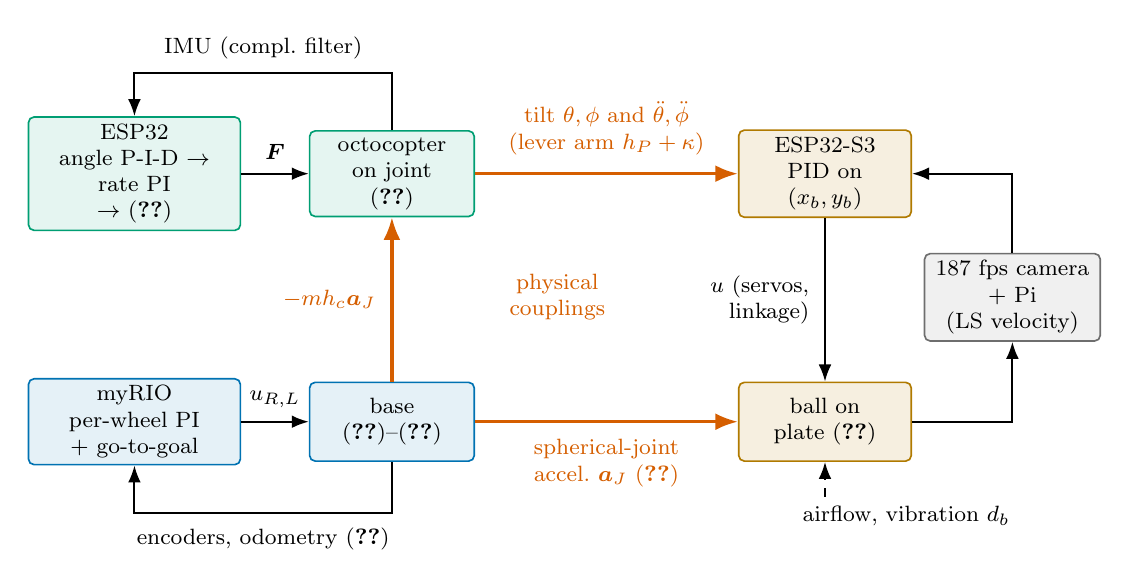
\begin{tikzpicture}[font=\footnotesize, >=Latex,
  blk/.style={draw, rounded corners=2pt, align=center, minimum height=10mm, inner xsep=3pt, inner ysep=2.5pt, line width=0.6pt, fill=#1},
  blk/.default=white]
  % base loop (x: 0.00..5.62)
  \node[blk=pAzul!10, draw=pAzul, text width=2.48cm] (bc) at (1.35, 0.00) {myRIO\\ per-wheel PI\\ + go-to-goal};
  \node[blk=pAzul!10, draw=pAzul, text width=1.88cm] (bp) at (4.62, 0.00) {base\\ \eqref{eq:basev}--\eqref{eq:motor}};
  \draw[->, line width=0.7pt] (bc) -- node[above=1.5pt]{$u_{R,L}$} (bp);
  \draw[->, line width=0.7pt] (bp.south) -- ++(0,-0.65) -| node[pos=0.25, below=1.5pt]{encoders, odometry \eqref{eq:odo}} (bc.south);

  % drone loop
  \node[blk=pVerde!10, draw=pVerde, text width=2.48cm] (dc) at (1.35, 3.15) {ESP32\\ angle P-I-D $\to$\\ rate PI\\ $\to$ \eqref{eq:alloc_inv}};
  \node[blk=pVerde!10, draw=pVerde, text width=1.88cm] (dp) at (4.62, 3.15) {octocopter\\ on joint\\ \eqref{eq:pitchlin}};
  \draw[->, line width=0.7pt] (dc) -- node[above=1.5pt]{$\vect F$} (dp);
  \draw[->, line width=0.7pt] (dp.north) -- ++(0,0.72) -| node[pos=0.25, above=1.5pt]{IMU (compl.\ filter)} (dc.north);

  % ball loop (x: 9.05..13.70)
  \node[blk=pOcre!12, draw=pOcre, text width=1.98cm] (cc) at (10.12, 3.15) {ESP32-S3\\ PID on\\ $(x_b,y_b)$};
  \node[blk=pOcre!12, draw=pOcre, text width=1.98cm] (bb) at (10.12, 0.00) {ball on\\ plate \eqref{eq:balllinx}};
  \node[blk=pGris!10, draw=pGris, text width=2.02cm] (cam) at (12.50, 1.58) {187 fps camera\\ + Pi\\ (LS velocity)};
  \draw[->, line width=0.7pt] (cc) -- node[left=2pt, align=right]{$u$ (servos,\\ linkage)} (bb);
  \draw[->, line width=0.7pt] (bb.east) -| (cam.south);
  \draw[->, line width=0.7pt] (cam.north) |- (cc.east);

  % physical couplings (red #D55E00)
  \draw[->, line width=1.15pt, pRojo] (bp.east) -- node[below=2.5pt, align=center]{spherical-joint\\ accel.\ $\vect a_J$ \eqref{eq:aJ}} (bb.west);
  \draw[->, line width=1.15pt, pRojo] (bp.north) -- node[left=2pt, align=right]{$-mh_c\vect a_J$} (dp.south);
  \draw[->, line width=1.15pt, pRojo] (dp.east) -- node[above=3pt, align=center]{tilt $\theta,\phi$ and $\ddot\theta,\ddot\phi$\\ (lever arm $h_P+\kappa$)} (cc.west);
  \node[pRojo, align=center] at (6.72, 1.58) {physical\\ couplings};

  % direct disturbance on the ball (without crossing any loop)
  \node[align=center] (dist) at (11.15, -1.20) {airflow, vibration $d_b$};
  \draw[->, dashed, line width=0.7pt] (dist.north -| bb.south) -- (bb.south);
\end{tikzpicture}
\caption{AeroTray's three control loops and their physical couplings (thick arrows). The octocopter controller regulates attitude relative to gravity; the ball controller tilts the plate relative to the octocopter; the camera is fixed to the octocopter.}
\label{fig:loops}
\end{figure}

\subsubsection{Octocopter attitude}
\label{sec:attitude}

\paragraph{Estimator and control law}
Attitude is estimated at \SI{200}{\hertz} by integrating the Euler-angle rates \eqref{eq:euler_rates} from the bias-corrected gyroscope and correcting toward accelerometer tilt with a complementary filter \cite{mahony2008}. The accelerometer is pre-filtered by a \SI{10}{\hertz} low-pass filter, the correction time constant is \SI{1}{\second} above \SI{1400}{\micro\second} (\SI{0.25}{\second} below), and correction is skipped when the filtered specific force deviates from $1\,g$ by more than $0.15\,g$, because rotor vibration reached $2\,g$. The controller is a cascade \cite{mahony2012,pounds2010}; for the pitch axis,
\begin{align}
  \dot\theta_{\mathrm{ref}}&=\sat_{\omega_{\lim}}\!\Big(-k_{p\theta}\,\theta-k_{d\theta}\,\dot\theta_f+k_{i\theta}\!\int\!(-\theta)\,\dd t\Big), \notag\\
  \tau_y&=k_{p\omega}(q_{\mathrm{ref}}-q)+k_{i\omega}\!\int\!(q_{\mathrm{ref}}-q)\,\dd t, \label{eq:cascade}
\end{align}
where $\dot\theta_f$ is the Euler-angle derivative filtered with a \SI{25}{\milli\second} time constant, $q_{\mathrm{ref}}$ is obtained from $(\dot\phi_{\mathrm{ref}},\dot\theta_{\mathrm{ref}})$ by inverting \eqref{eq:euler_rates}, and torques are allocated with \eqref{eq:alloc_inv}. The gains are $k_{p\theta}=\SI{4.62}{\per\second}$, $k_{d\theta}=0.12$, $k_{p\omega}=\SI{0.848}{\newton\metre\second\per\radian}$, $k_{i\omega}=\SI{0.10}{\newton\metre\per\radian}$, and $k_{i\theta}=0.8$ in bench mode and $2.0$ in flight mode. The commanded angular rate is limited to $\omega_{\lim}=\SI{25}{\degree\per\second}$ in bench mode and \SI{60}{\degree\per\second} in flight mode, and the rate integral to \SI{0.3}{\radian} and \SI{3.0}{\radian}, respectively. The yaw loop slowly returns to the initial heading ($\pm\SI{15}{\degree\per\second}$, $|\tau_z|\le\SI{0.06}{\newton\metre}$).

\paragraph{Linear stability}
Closing \eqref{eq:pitchlin} with \eqref{eq:cascade}, the thrust-gain ratio $k_T$, motor lag $\tau_m$, and actuation delay $T_a$ (Table~\ref{tab:params}), the inner loop $k_Tk_{p\omega}/(J_ys)$ crosses over at \SI{10}{\radian\per\second} with \SI{43}{\degree} of phase margin for $k_T=1.42$. The outer loop must overcome the negative stiffness of the inverted pendulum. Neglecting the slow integrators and fast actuator, the closed loop is $J_y\ddot\theta+c\dot\theta+(k_Tk_{p\omega}k_{p\theta}-mgh_c)\theta=0$, which is stable only if
\begin{equation}
  k_T\,k_{p\omega}\,k_{p\theta}>m\,g\,h_c .
  \label{eq:stiff}
\end{equation}
Figure~\ref{fig:dronestab}b shows the stability region of the full linear model (cascade, integrators, derivative filter, motor lag, and a second-order Pad\'e approximation of $T_a$) in the $(h_c,k_T)$ plane; its boundary lies only 6--12\% above \eqref{eq:stiff} and is nearly insensitive to $\pm25\%$ changes in $J_y$. At the identified values, the margin is tight: $k_Tk_{p\omega}k_{p\theta}=\SI{5.6}{\newton\metre\per\radian}$ versus $mgh_c=\SI{4.5}{\newton\metre\per\radian}$. Two consequences follow. First, had the firmware thrust map been exact ($k_T=1$), the loop would be unstable for $h_c>\SI{0.11}{\metre}$; the controller worked because the actual thrust gain exceeds the assumed value. Because $k_T$ scales with $V_{\mathrm{bus}}^2$ \eqref{eq:tv}, the same condition explains why battery discharge erodes stiffness margin: at 11.6\,V at rest, $k_T$ drops by 15\% and \eqref{eq:stiff} sits virtually on the boundary. Second, low net stiffness combined with the angle integrator creates a slow, lightly damped closed-loop mode: $\zeta=0.24$ at \SI{0.30}{\hertz} with flight gains and $\zeta=0.42$ at \SI{0.20}{\hertz} with the bench integral gain. Hover attitude spectra peak at 0.15--\SI{0.23}{\hertz} (4--7\,s periods), in agreement with this mode.

\paragraph{Torque authority and region of attraction}
\label{sec:authority}
When the commanded angular rate saturates, the quasi-static restoring torque cannot exceed
\begin{equation}
  \tau_{\mathrm{avail}}=k_T\big(k_{p\omega}\,\omega_{\lim}+k_{i\omega}\,I_{\lim}\big),
  \label{eq:tauavail}
\end{equation}
whereas holding a tilt $\theta$ requires $mg(\delta_x+h_c\sin\theta)$ by \eqref{eq:pitchlin}. Recovery is impossible beyond
\begin{equation}
  \theta^\ast=\arcsin\!\Big(\frac{\tau_{\mathrm{avail}}/(mg)-\delta_x}{h_c}\Big).
  \label{eq:thetastar}
\end{equation}
Under the bench limits of firmware v4--v7, $\tau_{\mathrm{avail}}=0.40k_T=$ 0.53--\SI{0.61}{\newton\metre} and $\theta^\ast=$ 2.8--\SI{3.8}{\degree} for the identified $h_c$ (2.0--\SI{6.7}{\degree} across its uncertainty interval): no liftoff transient larger than a few degrees could recover, and the module drifted slowly into the \SI{12}{\degree} interlock, as observed in Flights~3--6 (Fig.~\ref{fig:dronestab}a). The flight limits of v8--v9 raise $\tau_{\mathrm{avail}}$ to 1.6--\SI{1.8}{\newton\metre} and $\theta^\ast$ to 16--\SI{19}{\degree}, beyond the interlock; the next two flights remained airborne. The decisive change was therefore the angular-rate limit rather than the gains, consistent with the identical behavior of v5 (full gains) and v6 (75\% gains). Neither limit comes from the motors: by \eqref{eq:taumax}, the allocator can deliver over \SI{2.4}{\newton\metre} below \SI{1816}{\micro\second}.

\begin{figure}[!htbp]
  \centering
  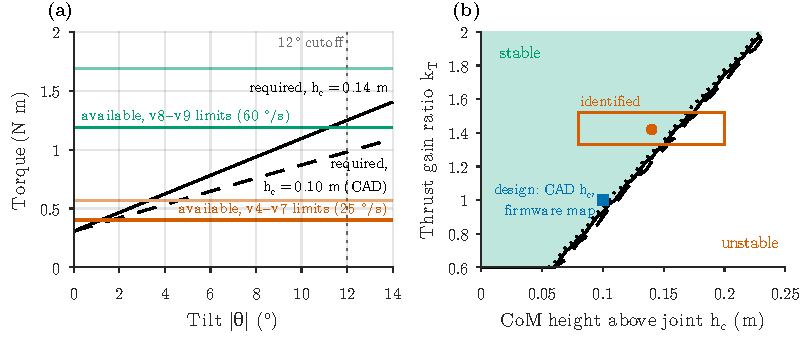
\includegraphics{figures/fig_drone_stability.pdf}
  \caption{Octocopter attitude loop. (a) Gravity torque required to hold a tilt (identified and CAD values of $h_c$) and available torque under angular-rate saturation \eqref{eq:tauavail}, for bench and flight limits; thick lines $k_T=1$, thin lines $k_T=1.42$. (b) Stability region of the full linear model in the $(h_c,k_T)$ plane; boundaries are drawn for $J=0.12$ (solid), 0.09 (dashed), and \SI{0.15}{\kilo\gram\metre\squared} (dotted). The rectangle marks the identified uncertainty and the square marks the design point (CAD $h_c$, firmware map).}
  \label{fig:dronestab}
\end{figure}

\subsubsection{Ball and plate}
\label{sec:ballcontrol}

\paragraph{Control law}
For each axis and each received camera frame, the ESP32-S3 computes
\begin{equation}
  u=u_n+\sat_{\pm220}\Big(k_p\,e+k_i\!\int\!e\,\dd t-k_d\,\hat v\Big),\qquad e=-x_b,
  \label{eq:ballpid}
\end{equation}
with velocity $\hat v$ from \eqref{eq:lsvel} computed by the Pi. The firmware works in \SI{3}{\milli\metre} units; in SI-consistent units, the gains $(1.5;\ 0.8;\ 4.5)$ become $k_p=\SI{0.50}{\micro\second\per\milli\metre}$, $k_i=\SI{0.27}{\micro\second\per\milli\metre\per\second}$, and $k_d=\SI{1.5}{\micro\second\per\milli\metre\second}$. Neutral pulse widths are $u_n=(1386;\ 1392)$\,\si{\micro\second}, the integral is clamped at 90\% of the output range, and the backlash from Section~\ref{sec:linkage} is added with a \SI{30}{\micro\second} ramp.

\paragraph{Discrete-time stability analysis}
Because the derivative acts through an FIR filter and the loop contains several pure delays (frame exposure and transfer, image processing, the \SI{50}{\hertz} servo frame, and analog-servo dead time), the loop was analyzed in discrete time at the camera period $h$: plant \eqref{eq:balltf} with a servo lag $\tau_s=\SI{50}{\milli\second}$ was discretized with a zero-order hold, total delay $T$ was represented by $T/h$ unit delays, the derivative used the exact FIR \eqref{eq:lsvel}, the integral used forward Euler, and stability was decided from the roots of the closed-loop characteristic polynomial. Figure~\ref{fig:ballstab}a shows the largest stable $k_d$ (in firmware units) versus $T$ for several plant gains. At the CAD gain $K_b=6.0$, the nominal $k_d=4.5$ is stable only if $T\lesssim\SI{40}{\milli\second}$---less than the sum of frame, processing, \SI{50}{\hertz} servo-frame, and servo dead-time delays. On the bench with rotors off, $k_d=4.5$ was stable and $k_d=6$ was unstable; for plausible delays ($T=$ 60--\SI{180}{\milli\second}), the model reproduces both observations only with an effective gain $K_{b,\mathrm{eff}}=3.5$--4.9 (58--82\% of the CAD value), where higher gains correspond to shorter delays. This reduction agrees with linkage backlash, whose describing function lowers small-signal gain, and with a direct regression of ball acceleration on logged servo pulses, which gives 2.5 and 4.9 for the $x$ and $y$ axes ($R^2=0.29$ and 0.45, limited by the 20\,Hz pulse logging rate). At $K_{b,\mathrm{eff}}=4.2$ and $T=\SI{0.10}{\second}$, the closed loop has a lightly damped fast mode at \SI{1.3}{\hertz} ($\zeta=0.06$), the signature of operating near the delay limit, and a slow integral mode at \SI{0.064}{\hertz} ($\zeta=0.37$, \SI{16}{\second} period).

\begin{figure}[!htbp]
  \centering
  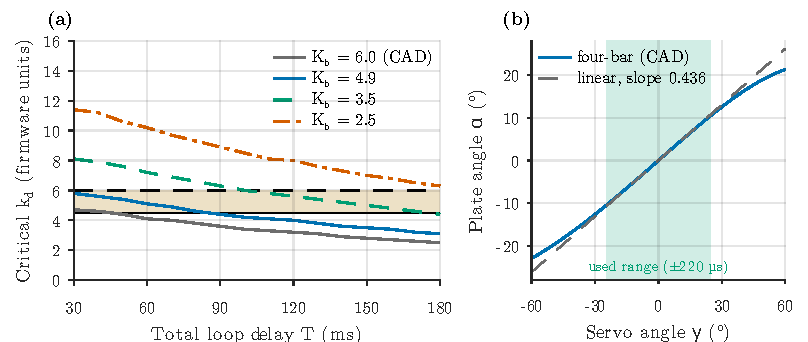
\includegraphics{figures/fig_ball_stability.pdf}
  \caption{Ball and plate. (a) Largest stable derivative gain (firmware units, $k_p=1.5$, $k_i=0.8$) versus total loop delay for four plant gains; the shaded band is bounded by the gain that was stable on the bench ($k_d=4.5$, solid line) and the one that was unstable ($k_d=6$, dashed). (b) Plate angle versus servo angle from the closed-form four-bar solution \eqref{eq:freud} and its linearization.}
  \label{fig:ballstab}
\end{figure}

\subsubsection{Mobile base}
\label{sec:basecontrol}
Each wheel runs a velocity PI loop with conditional integration (the integral freezes when the output saturates at 0 or 100\% duty cycle) using \SI{1}{\kilo\hertz} PWM. Go-to-goal mode uses the polar error $\rho=\|\vect p_g-\vect p\|$, $e_\psi=\operatorname{atan2}(\Delta y,\Delta x)-\psi$, whose kinematics follow from \eqref{eq:diff}: $\dot\rho=-v\cos e_\psi$, $\dot e_\psi=-\omega+(v/\rho)\sin e_\psi$. The law sets $\omega=\sat_{0.2}(1.2e_\psi)$, with $v=0$ while $|e_\psi|>\SI{0.2}{\radian}$ and $v=\min\{0.05;\ \max(0.025;\ 0.8\rho)\}$\,m/s otherwise, stopping once $\rho<\SI{2}{\centi\metre}$. Because no smooth time-invariant feedback can stabilize the full pose of a unicycle \cite{brockett1983}, the law regulates position only; convergence follows from elementary bounds. During the turning phase, $|e_\psi|$ decreases at no less than \SI{0.2}{\radian\per\second} until $|e_\psi|\le0.2$. During the approach phase, $\dot\rho\le-0.025\cos0.2<0$, and $V=e_\psi^2/2$ satisfies $\dot V\le-(\omega/e_\psi-v/\rho)\,e_\psi^2$ with $\omega/e_\psi\ge1$ and $v/\rho\le0.8$ for $\rho\ge\SI{3.1}{\centi\metre}$, so $|e_\psi|$ does not grow and the robot reaches the target tolerance in finite time after at most one turning phase.

\subsubsection{Octocopter altitude and heading (firmware v11)}
\label{sec:altura}
\paragraph{Heading on the base} The octocopter operates independently and receives no data from the base. At idle ($\le\SI{1400}{\micro\second}$), while mounted on the base, it holds its startup heading within a $\pm\SI{20}{\degree}$ \emph{sliding window}. If a base turn drags it past that limit, the reference slides with it instead of cutting the motors. It therefore does not fight the spherical joint during a \SI{360}{\degree} turn, and when the base stops it settles with at most a \SI{20}{\degree} offset. A safety cutoff remains active at \SI{120}{\degree\per\second}. Above \SI{1400}{\micro\second}, v9 behavior is retained: fixed heading hold with cutoffs at \SI{20}{\degree} and \SI{35}{\degree\per\second}. Under v9, base turns ended in the \SI{20}{\degree} cutoff.

\paragraph{Altitude measurement} The VL53L0X produced no valid readings during the 20 November flights. \SI{80}{\percent} of readings returned code~2 (\emph{signal fail}): the return signal from the laboratory floor (0.06--\SI{0.3}{MCPS}) fell below ambient infrared light (0.7--\SI{0.99}{MCPS}). Four measures were applied:
\begin{enumerate}[label=(\roman*)]
  \item a matte white \emph{target} (an A4 sheet) fixed to the base beneath the sensor, boosting signal return by a factor of 2 to 10; mounted on the base, the laser measures module position along the vertical guide---the variable of interest---independent of the floor or ramp;
  \item the sensor's long-range profile, with a \SI{0.05}{MCPS} signal limit, up to \SI{60}{\milli\metre} sigma, and \SI{66}{\milli\second} per reading;
  \item a three-reading median filter rejecting jumps larger than \SI{60}{\milli\metre};
  \item a linear ruler calibration at two guide heights: $d=0.930\,d_m-\SI{36.5}{\milli\metre}$.
\end{enumerate}
Accepted readings rose from \SI{0}{\percent} to nearly \SI{100}{\percent}, yielding 317--\SI{334}{\milli\metre} against \SI{330}{\milli\metre} measured with a ruler.

\paragraph{Sensor lever-arm correction} The laser sits on arm~8 ($+x$) at a horizontal distance $r_s$ from the spherical joint axis. When the module pitches by $\theta$ (positive nose-down, $+x$ downward in the FLU convention) or rolls by $\phi$, its tip moves vertically by $r_s\sin\theta$, altering the measured distance $d$ even when the spherical joint does not move along the guide. The axis height is
\begin{equation}
  z=d\cos\phi\cos\theta+r_s\sin\theta ,
  \label{eq:brazo}
\end{equation}
which feeds the filter. With $r_s=\SI{0.20}{\metre}$ (measured), a \SI{2}{\degree} pitch oscillation produces an apparent \SI{7}{\milli\metre} height shift without correction ($0.20\sin 2^\circ\approx\SI{7.0}{\milli\metre}$); the firmware applies \eqref{eq:brazo} to every reading before filtering. For the same reason, the IMU accelerometer, also on arm~8, measures the tangential and centripetal accelerations of module rotation ($\dot{\vect\omega}\times\vect r_s+\vect\omega\times(\vect\omega\times\vect r_s)$). At hover angular rates below \SI{10}{\degree\per\second}, this term is smaller than \SI{0.05}{\metre\per\second\squared} and falls within the filter's process noise.

\paragraph{Altitude Kalman filter} Altitude is estimated by fusing the laser with the accelerometer. The state is $\vect x=[z,\ v,\ b]^{\top}$, where $z$ is the distance to the target, $v$ is vertical velocity, and $b$ is vertical accelerometer bias. Prediction runs at the IMU rate using world-frame vertical acceleration from the \SI{10}{\hertz}-filtered accelerometer and estimated attitude:
\begin{equation}
  \begin{gathered}
    a_z=\big(-\sin\theta\,a_x+\sin\phi\cos\theta\,a_y+\cos\phi\cos\theta\,a_z^{b}\big)g-g,\\
    z_{k+1}=z_k+v_k\Delta t+\tfrac12(a_z-b_k)\Delta t^2,\quad
    v_{k+1}=v_k+(a_z-b_k)\Delta t,\quad b_{k+1}=b_k .
  \end{gathered}
  \label{eq:kfz}
\end{equation}
Process noise is $\sigma_a=\SI{0.6}{\metre\per\second\squared}$ on acceleration and $\sigma_b=\SI{0.02}{\metre\per\second\squared}/\sqrt{\mathrm{s}}$ on bias. Each accepted laser reading updates the state with $R=(\SI{52}{\milli\metre})^2$, the dispersion measured over the floor. Updates pass through a $3\sigma$ gate, and the filter resynchronizes after five consecutive rejections. In simulation with measured noise, altitude error drops from \SI{73}{\milli\metre} (raw laser) to 33--\SI{52}{\milli\metre}. On the bench with the target, filter uncertainty is about \SI{23}{\milli\metre}.

\paragraph{Cascaded altitude control} The vertical plant is a double integrator, compounded by motor lag (\SI{70}{\milli\second}), sensor delay (\SI{66}{\milli\second} plus median filtering), and dry guide friction that causes stick--slip jumps. A single PID on altitude therefore oscillates. A cascade is used instead:
\begin{equation}
  \begin{gathered}
    v_{\mathrm{ref}}=\mathrm{sat}_{\pm\SI{40}{\milli\metre\per\second}}\!\big(k_z(z_{\mathrm{ref}}-\hat z)\big),\\
    \Delta u=\mathrm{sat}_{\pm\SI{60}{\micro\second}}\!\Big(k_{vp}(v_{\mathrm{ref}}-\hat v)+k_{vi}\!\int(v_{\mathrm{ref}}-\hat v)\,dt\Big),
  \end{gathered}
  \label{eq:cascada}
\end{equation}
with $k_z=\SI{1.5}{\per\second}$, $k_{vp}=\SI{0.18}{\micro\second\per(\milli\metre\per\second)}$, $k_{vi}=\SI{0.35}{\micro\second\per\milli\metre}$, and integrator anti-windup. The reference $z_{\mathrm{ref}}$ follows the target along a \SI{20}{\milli\metre\per\second} ramp; the \emph{Subir} (Up) and \emph{Bajar} (Down) commands step it by $\pm\SI{20}{\milli\metre}$. The inner loop uses velocity from the Kalman filter, avoiding the lag of differentiating laser readings so the module brakes before arrival. Its integrator compensates for battery voltage sag and friction.

In simulation with Coulomb friction and stick--slip in the guide, peak-to-peak oscillation drops from 13--\SI{46}{\milli\metre} with PID to 4--\SI{12}{\milli\metre} with the cascade. Altitude hold activates via \emph{Mantener} (Hold) only if filter uncertainty is below \SI{30}{\milli\metre}; otherwise the collective stays fixed. Flight validation remains pending.

\subsection{Coupled model and disturbance propagation}
\label{sec:coupling}

Combining the linearized octocopter \eqref{eq:pitchlin} closed with \eqref{eq:cascade} and the ball \eqref{eq:balllinx} closed with \eqref{eq:ballpid} gives the propagation from base acceleration to ball position:
\begin{gather}
  X_b(s)=\frac{S_b(s)}{s^2}\Big\{\gamma_b\Big[\big(g-(h_P+\kappa)s^2\big)\,T_{\theta A}(s)-1\Big]A_{J,x}(s)+D_b(s)\Big\}, \label{eq:propag}\\
  T_{\theta A}(s)=\frac{-m h_c\,P(s)}{1+L_D(s)}, \notag
\end{gather}
where $P(s)=1/(J_ys^2-mgh_c)$, $L_D$ is the open-loop transfer function of the attitude cascade, $S_b=1/(1+L_b)$ is the sensitivity of the ball loop, and $D_b$ gathers all disturbances acting directly on the ball (airflow, vibration, backlash). Figure~\ref{fig:transm} evaluates \eqref{eq:propag}. Three findings stand out.

\begin{enumerate}[label=(\roman*)]
  \item \textbf{Rotation and slope are benign.} Centripetal acceleration of the spherical joint during the course-guide turns (wheel speeds up to \SI{0.10}{\metre\per\second}) is at most \SI{0.024}{\metre\per\second\squared} about the axle midpoint and \SI{0.015}{\metre\per\second\squared} about one wheel, equivalent to less than \SI{0.15}{\degree} of plate tilt; slope does not enter the ball equation \eqref{eq:tilt} at all. Only ramp transitions and base starts and stops produce significant accelerations.
  \item \textbf{The octocopter amplifies slow base accelerations.} Because its net stiffness \eqref{eq:stiff} is small, the module responds to base accelerations near its slow mode (0.2--\SI{0.3}{\hertz}) with tilts of several degrees per m/s$^2$ (Fig.~\ref{fig:transm}b), and between 0.1 and \SI{1}{\hertz} this path dominates over the direct path to the ball (Fig.~\ref{fig:transm}c). This agrees with the tilt cutoffs at the ramp edges in the integrated tests. It is the dynamic cost of a drone compared to a rigid gimbal (Section~\ref{sec:porquedron}).
  \item \textbf{Attitude motion is not the main source of ball error.} Filtering the measured octocopter attitude at idle (bench log, RMS 0.23--\SI{0.37}{\degree}) through $X_b/\Theta$ predicts a ball RMS of only 1.7--\SI{2.1}{\milli\metre}, whereas measured RMS with rotors spinning and base stationary is 16--\SI{21}{\milli\metre} in $x$ and 10--\SI{12}{\milli\metre} in $y$. Over 90\% of the measured variance lies below \SI{0.3}{\hertz}, with spectral peaks between 0.02 and \SI{0.05}{\hertz} (20--45\,s periods), the timescale of the ball loop's slow integral mode (\SI{0.064}{\hertz}). The dominant disturbance is therefore a slowly varying load acting directly on the ball ($D_b$): rotor airflow over the plate, vibration-induced drift, and backlash, which pulled the ball toward $(-x,-y)$ during tests. Only integral action rejects it, and its bandwidth is limited by delay.
\end{enumerate}

\begin{figure}[!htbp]
  \centering
  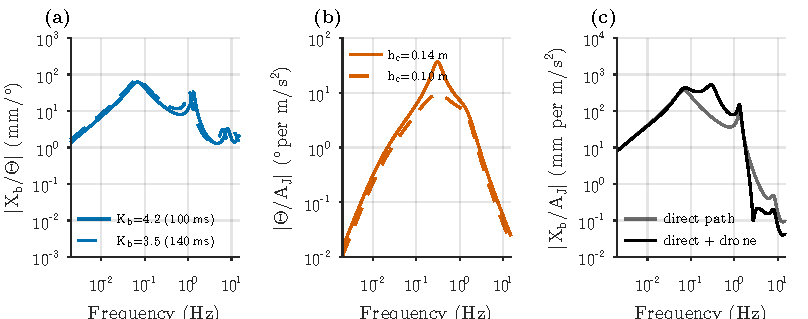
\includegraphics{figures/fig_transmissibility.pdf}
  \caption{Disturbance propagation predicted by \eqref{eq:propag} (hover gains, $k_T=1.42$). (a) Ball displacement per degree of octocopter tilt with the ball loop closed. (b) Octocopter tilt per unit base acceleration. (c) Ball displacement per unit base acceleration, via the direct path and through the octocopter.}
  \label{fig:transm}
\end{figure}

\subsection{Fundamental limitations and design implications}
\label{sec:limits_fund}
The model also bounds what any controller can achieve with the current hardware \cite{skogestad2005}.
\begin{itemize}
  \item \textbf{Octocopter.} An unstable pole $p$ demands a crossover above $\approx2p$, while an effective delay $\theta_e$ caps it at $\approx1/\theta_e$; robust stabilization requires roughly $p\,\theta_e<0.5$. With $p=\SI{6.1}{\radian\per\second}$ and $\theta_e\approx\tau_m+T_a=\SI{0.09}{\second}$, $p\theta_e=0.55$: attitude control on the spherical joint operates at the edge of this limit. The structural remedy is to lower the center of mass: with the batteries below the spherical joint ($h_c<0$), the module becomes a stable pendulum and the torque authority demanded by \eqref{eq:thetastar} decreases; low-mounted batteries would also improve tip-over stability on the ramp.
  \item \textbf{Ball and plate.} The right-half-plane zero $z_1=\SI{15.2}{\radian\per\second}$ limits crossover to $\approx z_1/2=\SI{7.6}{\radian\per\second}$, and the $\approx$\SI{0.1}{\second} delay limits it to $\approx\SI{10}{\radian\per\second}$; the PID operates at $K_{b,\mathrm{eff}}k_d\approx\SI{6}{\radian\per\second}$, near both bounds, explaining the ceiling on $k_d$. Faster ball control requires lower delay (\SI{333}{\hertz} digital servos, frame-synchronized servo updates) and smaller $\kappa$ (moving the plate surface closer to the universal joint center).
  \item \textbf{Mobile base.} Both the acceleration margin \eqref{eq:tip} and the octocopter's slow mode call for smooth (jerk-limited) base references; on a \SI{20}{\degree} slope, the thrust-free acceleration margin is only \SI{0.26}{\metre\per\second\squared}, rising to 0.7--\SI{1.0}{\metre\per\second\squared} when the rotors support 35--55\% of the module weight (Section~\ref{sec:porquedron}). Alternatives are low-mounted ballast or a lower aerial module.
  \item \textbf{Power.} Thrust margin drops with the square of battery voltage (Section~\ref{sec:bateria}); without voltage sensing and collective compensation, usable hover time is 3--\SI{7}{\minute} per LiPo pair.
\end{itemize}
   % 3. Model: coupling, control, and limits
%% ======================================================================
%% 05_design_files.tex -- 4. Design files summary
%% ======================================================================
\section{Design files summary}
\label{sec:designfiles}
All files are hosted in the repository \repourl. Table~\ref{tab:designfiles} summarizes the main design files.

\begin{small}
\begin{longtable}{@{}>{\raggedright\arraybackslash}p{0.36\textwidth}>{\raggedright\arraybackslash}p{0.13\textwidth}>{\raggedright\arraybackslash}p{0.12\textwidth}>{\raggedright\arraybackslash}p{0.31\textwidth}@{}}
\caption{Design files summary.}\label{tab:designfiles}\\
\toprule
File & Type & License & Location / function \\
\midrule\endfirsthead
\toprule File & Type & License & Location / function \\ \midrule\endhead
\texttt{junta nuevo de 8 motores con camara.step} & STEP (383 parts) & CERN-OHL-S & \fn{02_cad/} (external archive, $>95$\,MB; \fn{.glb} in repo) -- full assembly \\
\fn{x8_UAV_R350_imprimible_bandeja_v5.stp} & STEP & CERN-OHL-S & \fn{02_cad/} (external archive, $>95$\,MB) -- octocopter frame, towers, and tray (3D printing) \\
\fn{ball_and_plate_camara.stp} & STEP & CERN-OHL-S & \fn{02_cad/recibidos/} -- plate, servo linkages, camera mount \\
\fn{aerotray_conjunto_cad.xml} & MuJoCo XML & MIT & \fn{06_simulacion/simulacion/} -- spherical-joint and guide model (Isaac Lab, Section~\ref{sec:flights}) \\
\fn{derive_ball.py}, \fn{derive_drone.py} & Python 3 (SymPy) & MIT & \fn{00_paper_HardwareX/.../scripts_modelo/} -- symbolic verification of the Section~\ref{sec:model} equations \\
\fn{analysis.py}, \fn{ball_dt.py}, \fn{chain.py}, \fn{params.py}, \fn{rampa.py}, \fn{bateria.py}, \fn{exportar_datos_matlab.py} & Python 3 & MIT & \fn{00_paper_HardwareX/.../scripts_modelo/} -- all model values in Sections~\ref{sec:model} and \ref{sec:modelval} \\
\fn{generar_todas.m}, \fn{estilo_paper.m}, \fn{fig_*.m} & MATLAB & MIT & \fn{00_paper_HardwareX/.../figuras_matlab_en/} -- all data and model figures \\
\fn{Marcadores_ArUco_y_Calibracion_Bandeja_A4.pdf} & PDF & CC BY 4.0 & \fn{01_guias_y_documentacion/imprimibles/} -- plate calibration sheet \\
\fn{captura_octo_m8_vuelo_guia.ino} (v11) & Arduino C++ & MIT & \fn{03_firmware/firmware/} -- octocopter attitude, base-heading, and guided-flight firmware \\
\fn{captura_octo_m8_banco_angulo_laser.ino} & Arduino C++ & MIT & \fn{03_firmware/firmware/} -- bench-test firmware (fixed collective) \\
\fn{ball_plate_esp32s3_platformio/src/main.cpp} & PlatformIO C++ & MIT & \fn{03_firmware/} -- ball PID and servos on the ESP32-S3 \\
\fn{seguidor.py}, \fn{comunicacion.py}, \fn{myrio_uart.py}, \fn{pagina_dron.py}, \fn{pagina_robot.py} & Python 3 & MIT & \fn{04_raspberry_pi/pi_control/} -- Raspberry Pi supervisor, vision, links, and web UI \\
\fn{config_pi.json}, \fn{ajustes.json}, \fn{arrancar.sh} & JSON, shell & MIT & \fn{04_raspberry_pi/pi_control/} -- configuration, gains, and startup loop \\
\fn{prueba_prueba.vi} (main), \fn{AeroTray_Control_Formula.vi}, \fn{CONTROL_TRAYECTORIA.vi}, \fn{Laboratorio2_Ejercicio1_Motores.lvproj} & LabVIEW 2019 & MIT & \fn{05_labview_myrio/Control_Robot_Movil/} -- myRIO base control, odometry, sequences, UART \\
\fn{cargar_vuelo_guia_desde_pi.sh}, \fn{subir_uart_a_pi.sh} & shell & MIT & \fn{03_firmware/firmware/}, \fn{04_raspberry_pi/pi_control/} -- flash the drone and deploy Pi code \\
\fn{comparar_vuelo_isaac.py}, \fn{make_figures.py}, \fn{bp_metrics.py} & Python 3 & MIT & \fn{07_herramientas/}, \fn{00_paper_HardwareX/scripts_repositorio/} -- metrics and figures for Section~\ref{sec:validation} \\
\fn{isaaclab_aerotray/} (\fn{env.py}, \fn{agent.py}) & Python & MIT & \fn{06_simulacion/simulacion/} -- Isaac Lab task and PPO agent \\
\fn{vuelo_*.csv}, \fn{dron_log_*.csv}, \fn{registro_*.csv}, \fn{salida.log} & CSV, text & CC BY 4.0 & \fn{08_datos_y_registros/} -- raw logs used in this article \\
\fn{GUIA_EQUIPO.md}, \fn{VUELO_GUIA.md}, \fn{UART_MYRIO.md} & Markdown & CC BY 4.0 & \fn{01_guias_y_documentacion/} -- operation and flight procedures \\
Proteus schematics (\fn{AeroTray_Esquematicos.pdsprj}, \fn{AeroTray_Esquematicos_vista_v2.pdf}, \fn{AeroTray_Fig_Comunicaciones.pdf}) & Proteus, PDF & CERN-OHL-S & \fn{02_cad/esquematicos_proteus/} -- 6-sheet hierarchical electrical and communications schematic (Section~\ref{sec:power}) \\
\fn{IMG_1867.mov}, \fn{IMG_1868.mov}, \fn{IMG_1869.mov} & 4K HEVC video & CC BY 4.0 & External archive (see README) -- flights 6 and 7 on Nov 20 (Section~\ref{sec:flights}) \\
\bottomrule
\end{longtable}
\end{small}
        % 4. Design files summary
%% ======================================================================
%% 06_bom.tex -- 5. Bill of materials summary
%% ======================================================================
\section{Bill of materials summary}
\label{sec:bom}
Table~\ref{tab:bom} lists the components of the final prototype. Costs are approximate unit prices in USD as of November 2026 from local and online suppliers. Items marked ``lab'' were provided by the university laboratory; their list prices are shown for reference.

\begin{small}
\setlength{\tabcolsep}{4pt}
\begin{longtable}{@{}>{\raggedright\arraybackslash}p{0.27\textwidth}r>{\raggedleft\arraybackslash}p{0.08\textwidth}>{\raggedleft\arraybackslash}p{0.08\textwidth}>{\raggedright\arraybackslash}p{0.13\textwidth}>{\raggedright\arraybackslash}p{0.16\textwidth}@{}}
\caption{Bill of materials (approximate costs).}\label{tab:bom}\\
\toprule
Component & Qty. & Unit (USD) & Total (USD) & Source & Material type \\
\midrule\endfirsthead
\toprule Component & Qty. & Unit (USD) & Total (USD) & Source & Material type \\ \midrule\endhead
\multicolumn{6}{@{}l}{\emph{N1 -- Mobile base}}\\
NI myRIO-1900 & 1 & 500 & 500 & lab & Electronics \\
TETRIX MAX chassis parts, 2 TorqueNADO motors with encoders, drive wheels, and omni wheels & 1 set & 230 & 230 & lab & Metal / electromech. \\
MDD10A H-bridge ($\geq$\SI{10}{\ampere}/channel) & 1 & 15 & 15 & local supplier & Electronics \\
TETRIX NiMH battery \SI{12}{\volt} \SI{3000}{\milli\ampere\hour} + \SI{20}{\ampere} fuse & 1 & 45 & 45 & lab & Power \\
Power bank \SI{5}{\volt}/\SI{3}{\ampere} + 5-to-\SI{12}{\volt} boost converter & 1 & 25 & 25 & local supplier & Power \\
Mast, vertical guide, and carriage (aluminum profile, 3D-printed parts) & 1 & 30 & 30 & local / printed & Metal, PLA \\
\multicolumn{6}{@{}l}{\emph{N2 -- Aerial module (octocopter)}}\\
Frame (3D-printed center plate and towers, 8 R350 arms) & 1 & 60 & 60 & printed / online & PLA, composite \\
Spherical joint & 1 & 10 & 10 & local supplier & Metal \\
A2212 920\,KV brushless motor & 8 & 18 & 144 & online & Electromech. \\
9450 propeller (CW/CCW pair) & 4 & 3 & 12 & online & Polymer \\
30\,A ESC without BEC & 8 & 10 & 80 & online & Electronics \\
3S \SI{3300}{\milli\ampere\hour} 25C LiPo battery & 2 & 35 & 70 & online & Power \\
ATO fuse holder + \SI{30}{\ampere} fuse, relay, \SI{1000}{\micro\farad}/\SI{25}{\volt} capacitor, 14\,AWG wire, XT60 & 2 & 12 & 24 & local supplier & Electrical \\
NodeMCU-32S (ESP32) & 1 & 8 & 8 & local supplier & Electronics \\
MPU-6050 IMU & 1 & 3 & 3 & local supplier & Electronics \\
VL53L0X time-of-flight sensor & 1 & 5 & 5 & local supplier & Electronics \\
XL4015 buck converter & 2 & 4 & 8 & local supplier & Electronics \\
\multicolumn{6}{@{}l}{\emph{N3 -- Ball-and-plate tray}}\\
PS3 Eye USB camera & 1 & 10 & 10 & online & Electronics \\
ESP32-S3 development board & 1 & 12 & 12 & local supplier & Electronics \\
Futaba S3003 servo & 2 & 10 & 20 & local supplier & Electromech. \\
Plate ($250\times220$~mm), linkages, camera towers & 1 & 15 & 15 & printed & PLA \\
Blue ball, \SI{27}{\milli\metre} & 1 & 1 & 1 & local & Polymer \\
\multicolumn{6}{@{}l}{\emph{N4 -- Supervisor, electronics distribution, and emergency stop}}\\
Raspberry Pi 3B+ + \SI{32}{GB} microSD & 1 & 55 & 55 & online & Electronics \\
3S 18650 pack with BMS (BT5 logic and BT6 servos) & 2 & 20 & 40 & local supplier & Power \\
Latching NC emergency-stop mushroom button, \SI{4}{\metre} twin-core cable, relays K3--K4, 1N4007 diodes, Wago terminals & 1 & 15 & 15 & local supplier & Electrical \\
USB cables, hub, connectors, fasteners, zip ties & 1 & 20 & 20 & local supplier & Misc. \\
\midrule
\multicolumn{3}{@{}l}{\textbf{Total (all items)}} & \textbf{1,457} & & \\
\multicolumn{3}{@{}l}{\textbf{Total excluding lab-supplied items}} & \textbf{682} & & \\
\bottomrule
\end{longtable}
\end{small}

\subsection{Economic viability}
\label{sec:costos}
Table~\ref{tab:costos} compares the aerial module against alternatives that perform the same function: leveling the plate while the base climbs a ramp. Alternative prices are approximate market references.

\begin{table}[!htbp]
\centering
\small
\caption{Cost and capability comparison of alternatives for the leveling stage.}
\label{tab:costos}
\begin{tabularx}{\textwidth}{@{}>{\raggedright\arraybackslash}p{0.26\textwidth}c>{\raggedright\arraybackslash}X>{\raggedright\arraybackslash}p{0.13\textwidth}>{\raggedright\arraybackslash}p{0.14\textwidth}@{}}
\toprule
Alternative & USD & Leveling at \SI{10}{\degree} and \SI{20}{\degree} & Torque on base & Adjustable ballast \\
\midrule
Servos only on the base (2 S3003) & $\sim$20 & at \SI{10}{\degree} uses \SI{93}{\percent} of stroke; not feasible at \SI{20}{\degree} & yes & no \\
Servo gimbal + IMU (2 MG996R, MPU-6050) & $\sim$30--50 & yes & yes & no \\
Brushless gimbal (Storm32 + 2 motors) & $\sim$80--150 & yes, with limited payload & yes & no \\
\textbf{Octocopter module (Table~\ref{tab:bom})} & $\sim$\textbf{425} & yes, gravity-referenced & \textbf{no} (spherical joint) & \textbf{yes} ($f=0$--1) \\
Commercial single-problem lab equipment (ball balancer, 3-DOF drone) & thousands & not mobile & --- & --- \\
\bottomrule
\end{tabularx}
\end{table}

For leveling alone, a servo gimbal is 8 to 14 times cheaper. The octocopter is justified by three capabilities that a gimbal lacks:
\begin{itemize}
  \item it does not transmit the base reaction to the ball;
  \item it leaves the servo stroke free to control the ball;
  \item its thrust acts as an adjustable ballast (weight relief) that lowers the center of mass and increases the tip-over angle (Section~\ref{sec:porquedron}).
\end{itemize}
It also turns the robot into a research platform for stacked equilibria. The total cost remains well below that of commercial laboratory equipment, which solves a single problem on a fixed base.
                 % 5. Bill of materials summary
%% ======================================================================
%% 07_build.tex -- 6. Build instructions
%% ======================================================================
\section{Build instructions}
\label{sec:build}

\paragraph{Tools}
\begin{itemize}
  \item hex keys and TETRIX wrenches;
  \item soldering iron, crimper for XT60 and Dupont connectors, multimeter, and DC clamp meter;
  \item FDM 3D printer (PLA, 0.2\,mm layer height, 30\% infill for the towers and linkages);
  \item a laptop with Arduino CLI (ESP32 core), PlatformIO, and LabVIEW 2019 with the myRIO Toolkit.
\end{itemize}

\paragraph{Safety}
Assemble and flash all boards with the LiPo batteries disconnected and propellers removed. Verify the spin direction of every motor without propellers before the first flight.

\begin{figure}[!htbp]
  \centering
  \begin{subfigure}[b]{0.24\textwidth}\centering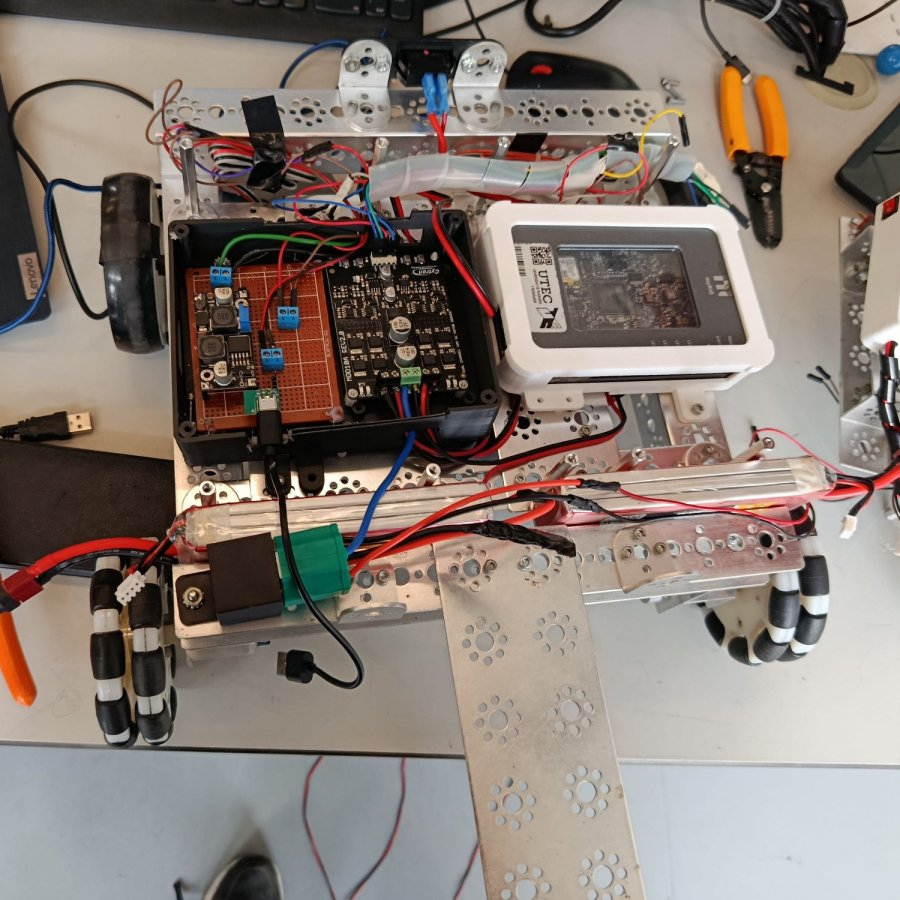
\includegraphics[width=\linewidth]{figures/paso1_base.jpg}\caption{Step 1: mobile base (myRIO, MDD10A, LiPo).}\end{subfigure}\hfill
  \begin{subfigure}[b]{0.24\textwidth}\centering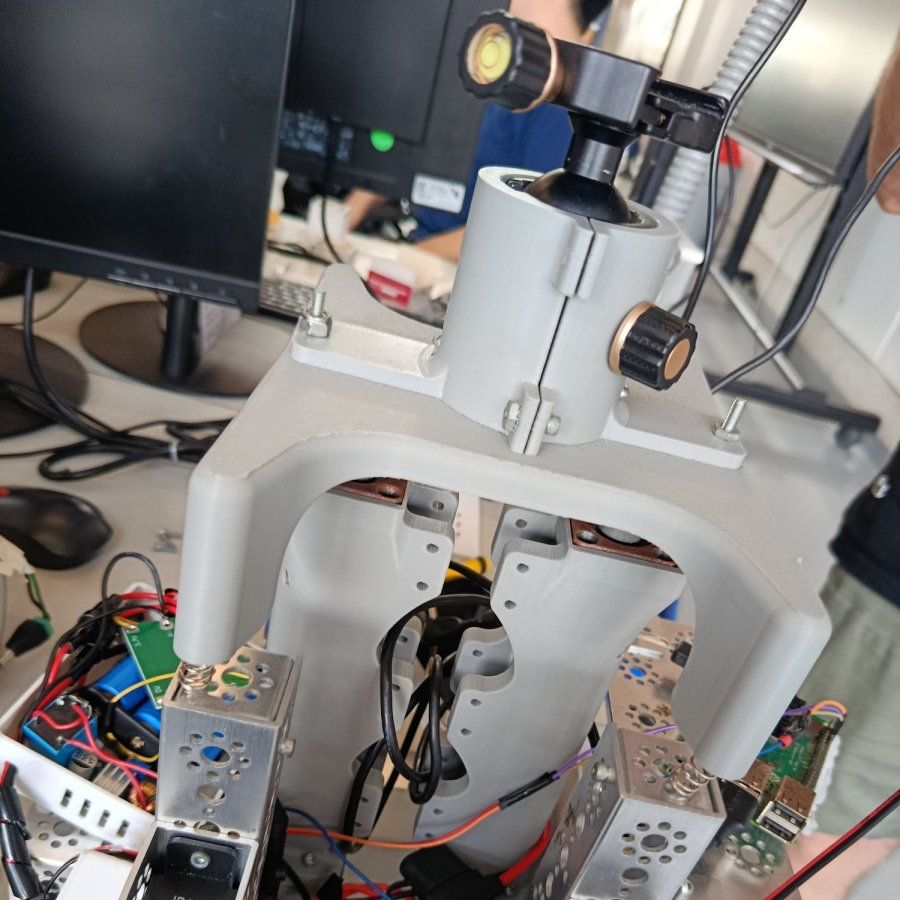
\includegraphics[width=\linewidth]{figures/paso2_mastil.jpg}\caption{Step 2: mast, guide, and spherical joint.}\end{subfigure}\hfill
  \begin{subfigure}[b]{0.24\textwidth}\centering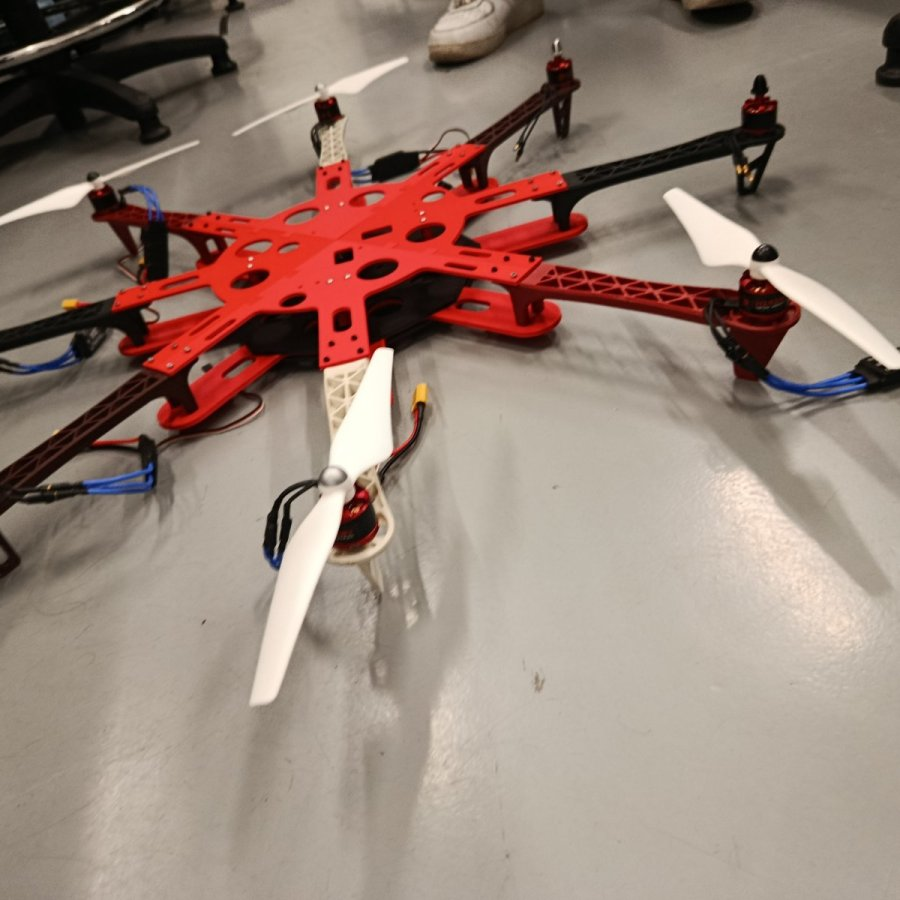
\includegraphics[width=\linewidth]{figures/paso3_marco.jpg}\caption{Step 3: eight-arm frame.}\end{subfigure}\hfill
  \begin{subfigure}[b]{0.24\textwidth}\centering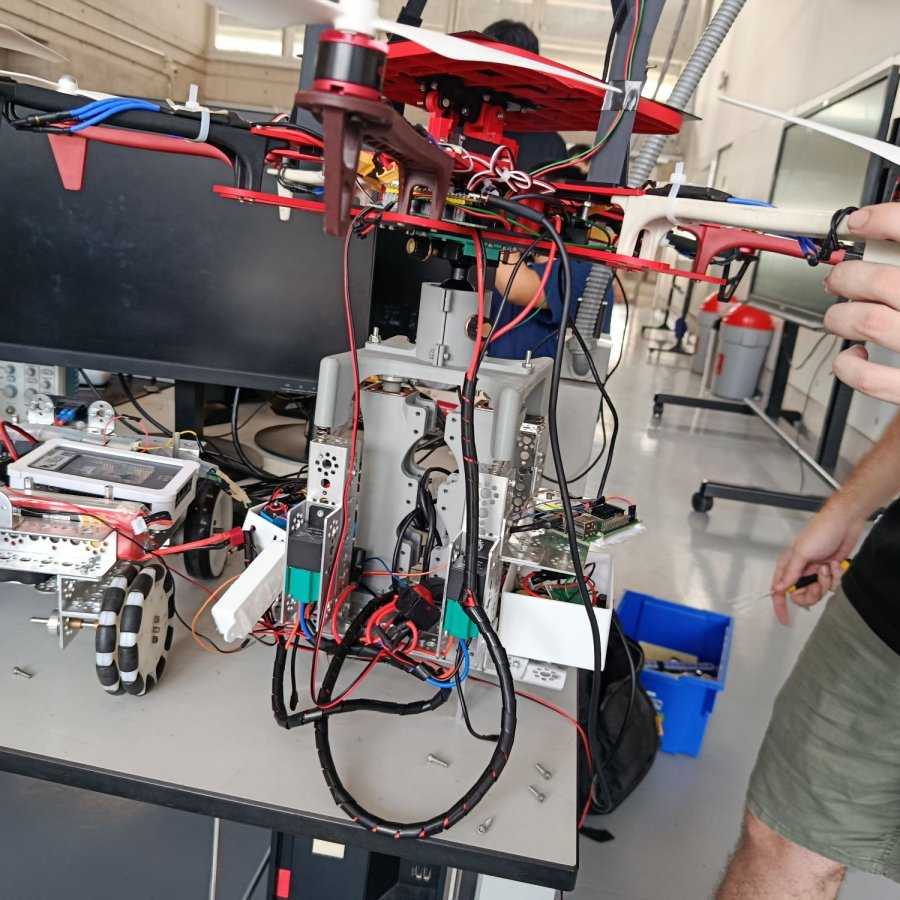
\includegraphics[width=\linewidth]{figures/paso4_dron_rotula.jpg}\caption{Step 4: drone mounted on the spherical joint.}\end{subfigure}\\[2mm]
  \begin{subfigure}[b]{0.24\textwidth}\centering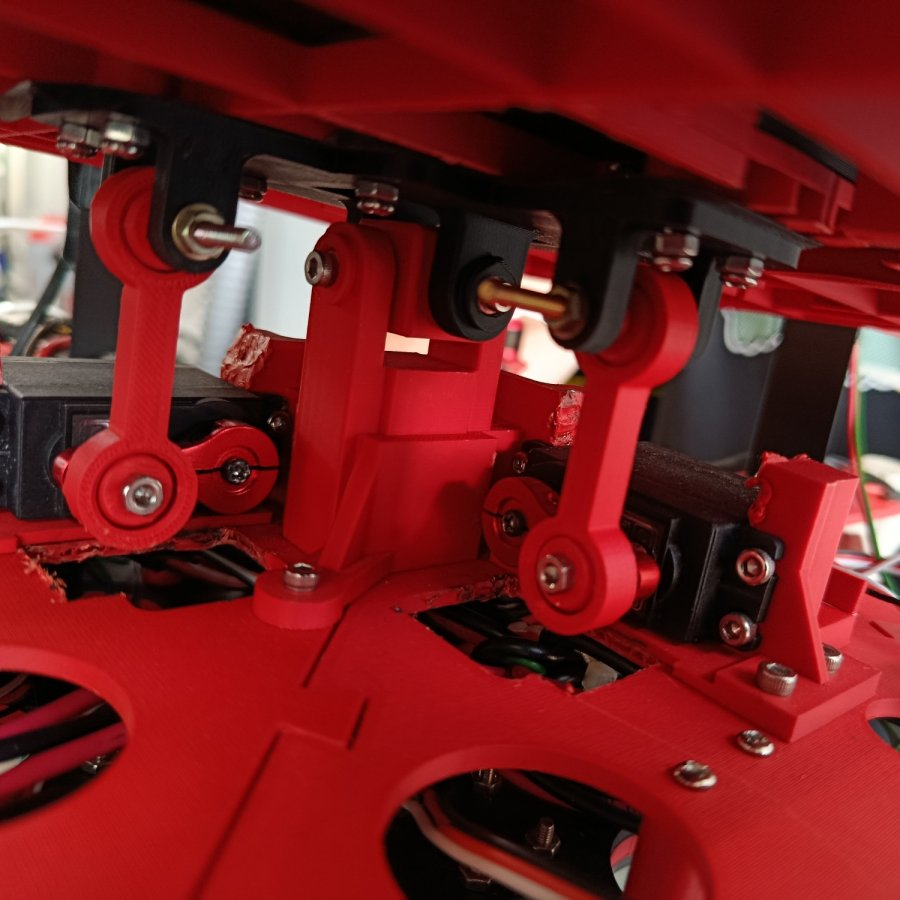
\includegraphics[width=\linewidth]{figures/paso5_mecanismo.jpg}\caption{Step 5: tray servos and linkages.}\end{subfigure}\hfill
  \begin{subfigure}[b]{0.24\textwidth}\centering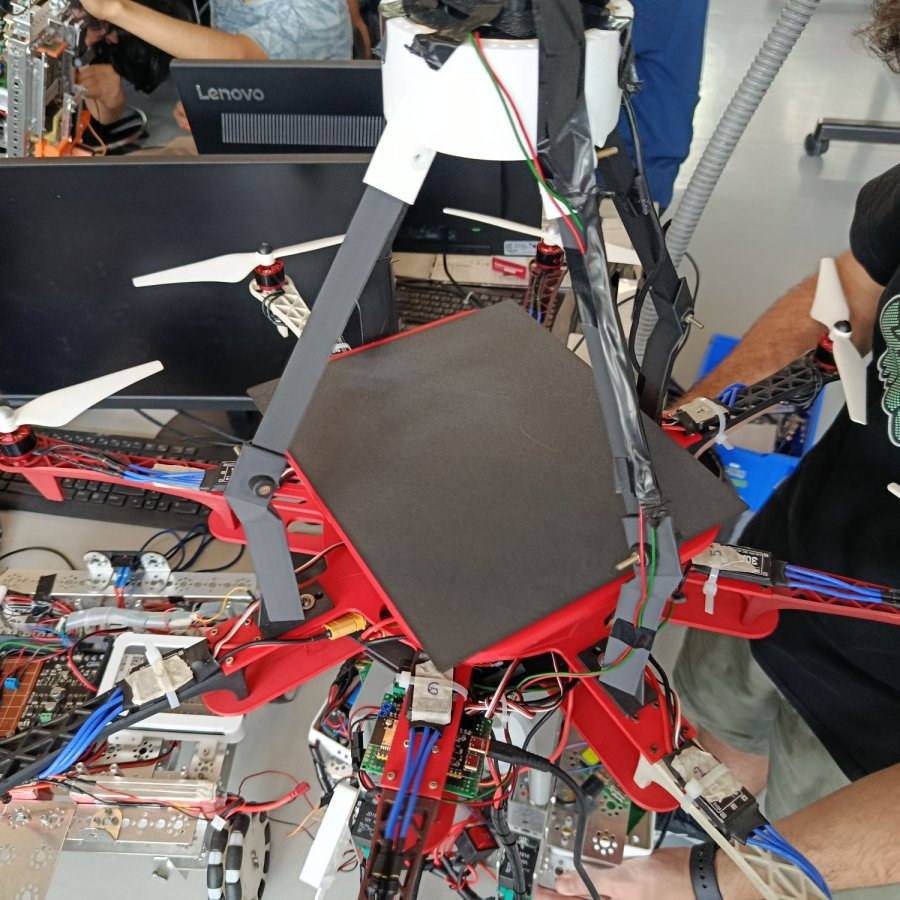
\includegraphics[width=\linewidth]{figures/paso5_bandeja_camara.jpg}\caption{Step 5: plate and camera towers.}\end{subfigure}\hfill
  \begin{subfigure}[b]{0.24\textwidth}\centering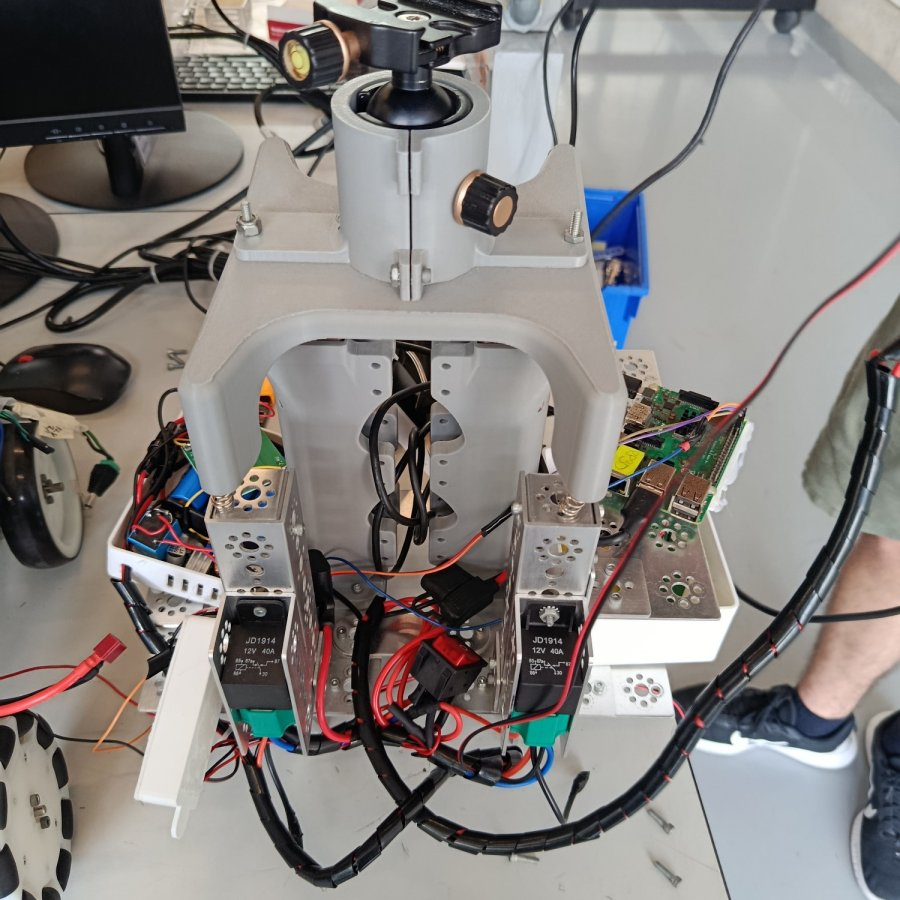
\includegraphics[width=\linewidth]{figures/paso6_supervisor.jpg}\caption{Step 6: emergency-stop relays and Raspberry Pi.}\end{subfigure}\hfill
  \begin{subfigure}[b]{0.24\textwidth}\centering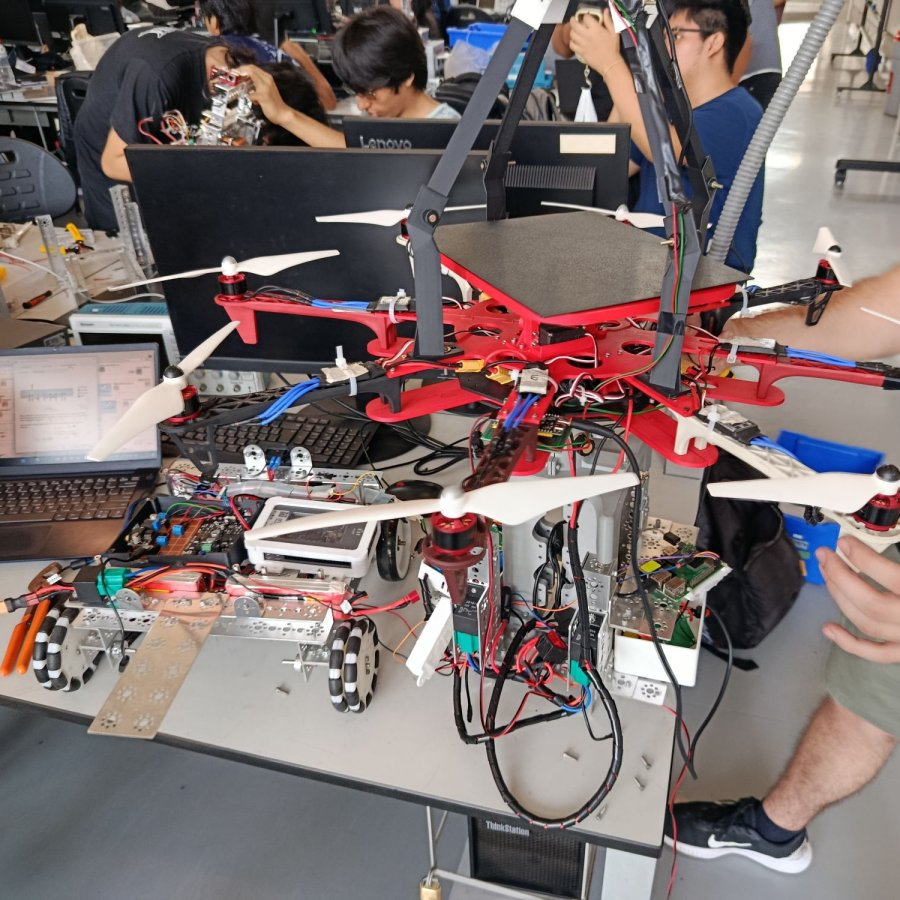
\includegraphics[width=\linewidth]{figures/paso7_integracion.jpg}\caption{Step 8: integration.}\end{subfigure}
  \caption{Build sequence of the final AeroTray prototype.}
  \label{fig:build}
\end{figure}

\begin{enumerate}[label=\textbf{Step \arabic*.}, leftmargin=*, align=left]
  \item \textbf{Mobile base (Fig.~\ref{fig:build}a).}
  \begin{enumerate}[label=(\alph*)]
    \item Assemble the TETRIX chassis with the two TorqueNADO motors on the rear axle and the omni wheels in front.
    \item Measure the track width (center-to-center distance between the drive wheels). It must match the value in the LabVIEW formula node, \SI{0.3794}{\metre}.
    \item Wire the left motor to myRIO MXP-A (PWM0 on pin 27, direction on DIO0, pin 11, encoder on ENC A/B) and the right motor to MXP-B on the same pins via the MDD10A.
    \item Protect the NiMH battery with the \SI{20}{\ampere} fuse and route it through the relay K3 contact.
    \item \emph{Check:} with the wheels off the ground, command forward motion and verify that both encoder counts increase. The right counter is inverted in software.
  \end{enumerate}

  \item \textbf{Mast, vertical guide, and spherical joint (Fig.~\ref{fig:build}b).}
  \begin{enumerate}[label=(\alph*)]
    \item Mount the vertical mast above the drive axle and attach the vertical guide.
    \item Insert the carriage with the spherical joint and verify approximately \SI{140}{\milli\metre} of free travel.
    \item Install soft end-stops at both ends of the guide.
    \item \emph{Check:} the carriage must drop freely under its own weight; guide friction biases the liftoff identification in Section~\ref{sec:ident}.
  \end{enumerate}

  \item \textbf{Octocopter frame and power (Fig.~\ref{fig:build}c).}
  \begin{enumerate}[label=(\alph*)]
    \item 3D-print the center plate and towers (file\\ \fn{x8_UAV_R350_imprimible_bandeja_v5.stp}) and mount the eight arms every \SI{45}{\degree}: M8 along $+x$, M7 along $+y$.
    \item Install M1--M4 as clockwise (CW) and M5--M8 as counterclockwise (CCW) (Table~\ref{tab:params}).
    \item Build the two independent power branches from the Rev.~I schematic (Section~\ref{sec:power}), each with a LiPo battery, XT60 connector, \SI{30}{\ampere} ATO fuse, relay contact 30--87 (K1, K2), 14\,AWG twisted pair, and a \SI{1000}{\micro\farad} capacitor at the drone. Branch A feeds ESCs 1, 3, 5, and 7; branch B feeds ESCs 2, 4, 6, and 8. Tie only the grounds together, and only at the drone.
    \item Cut the red (BEC) wire on all ESCs.
    \item Wire the ESC signals per Table~\ref{tab:pins} (firmware v11): NodeMCU-32S GPIO 25, 26, 27, 14, 21, 19, 5, and 17 for M1--M8; wire the MPU-6050 and VL53L0X to I$^2$C (SDA 23, SCL 22).
    \item Power the NodeMCU through the USB hub (logic domain). Do not add a regulator from the LiPo, as that would parallel two \SI{5}{\volt} supplies.
    \item Optional, recommended: solder VBAT voltage dividers to GPIO34/35 using R1 = R3 = \SI{10}{\kilo\ohm}, R2 = R4 = \SI{3.3}{\kilo\ohm} ($\div4.03$), and \SI{100}{\nano\farad} to GND so future firmware can measure battery voltage (Section~\ref{sec:bateria}).
  \end{enumerate}

  \item \textbf{Drone on the spherical joint (Fig.~\ref{fig:build}d).}
  \begin{enumerate}[label=(\alph*)]
    \item Bolt the frame to the spherical joint so the joint center coincides with the frame center.
    \item Balance the assembly so it sits level with the motors off. Shift the batteries until balanced and keep them as low as possible, because the center-of-mass height above the spherical joint sets the module's instability (Section~\ref{sec:limits_fund}). The prototype retains a \SI{9.5}{\milli\metre} residual eccentricity toward M8, identified in Section~\ref{sec:ident}.
  \end{enumerate}

  \item \textbf{Tray (Fig.~\ref{fig:build}e,f).}
  \begin{enumerate}[label=(\alph*)]
    \item 3D-print the plate, the linkages, and the four camera towers.
    \item Mount the two S3003 servos and connect their signal lines to GPIO47 ($x$) and GPIO21 ($y$) on the ESP32-S3.
    \item Power the servos from domain S5 (BT6, XL4015, relay K4 contact) with \SI{1000}{\micro\farad} at the input and a common ground with the ESP32-S3; do not connect the ESP32-S3 \SI{5}{\volt} pin to this rail.
    \item Mount the PS3 Eye on the towers, centered above the plate, and adjust the linkages so the plate sits level near \SI{1390}{\micro\second}.
  \end{enumerate}

  \item \textbf{Supervisor and emergency stop (Fig.~\ref{fig:build}g).}
  \begin{enumerate}[label=(\alph*)]
    \item Install Raspberry Pi OS (Debian 13) and create a virtual environment \texttt{\textasciitilde/venv} with \texttt{opencv-python}, \texttt{numpy}, \texttt{pyserial}, and \texttt{esptool}.
    \item Copy \texttt{pi\_control/} into the home directory.
    \item Enable the hardware UART: in \texttt{raspi-config}, set the serial login shell to \emph{No} and serial port hardware to \emph{Yes}, then reboot.
    \item Wire GPIO14 (TX, pin 8) to MXP-A pin 10 (RX), GPIO15 (RX, pin 10) to MXP-A pin 14 (TX), and GND (pin 6) to MXP-A pin 12.
    \item Power the Pi from its dedicated 3S 18650 pack (BT5) via an XL4015 set to \SI{5.2}{\volt}.
    \item Wire the control box: latching NC emergency-stop button SB1 in series with the K1--K4 coils powered from BT6 through a \SI{1}{\ampere} fuse, with a 1N4007 flyback diode across each coil. \emph{Check:} with SB1 pressed, no branch may have voltage downstream of its relay.
  \end{enumerate}

  \item \textbf{Firmware.}
  \begin{enumerate}[label=(\alph*)]
    \item Compile the drone firmware:\\ \texttt{arduino-cli compile --fqbn esp32:esp32:nodemcu-32s}.
    \item Flash it from the Pi using \fn{cargar_vuelo_guia_desde_pi.sh}, which runs \texttt{esptool write-flash 0x0}.
    \item Flash the ESP32-S3 with PlatformIO.
    \item Deploy the LabVIEW project to the myRIO (\fn{prueba_prueba.vi} as the main VI).
  \end{enumerate}

  \item \textbf{Integration checks (Fig.~\ref{fig:build}h).}
  \begin{enumerate}[label=(\alph*)]
    \item Launch \texttt{arrancar.sh} and open \url{http://<pi-ip>:8080/robot}. The log must display the drone firmware banner, \texttt{UART conectada en /dev/serial0} (UART connected), and the camera frame rate.
    \item With the battery disconnected, send \texttt{cal} and verify \texttt{CAL OK}.
    \item Place the ball on the plate and verify detection in all four corners.
  \end{enumerate}
\end{enumerate}
               % 6. Build instructions
%% ======================================================================
%% 08_operation.tex -- 7. Operation instructions
%% ======================================================================
\section{Operation instructions}
\label{sec:operation}

\begin{figure}[!htbp]
  \centering
  \begin{subfigure}[b]{0.52\textwidth}\centering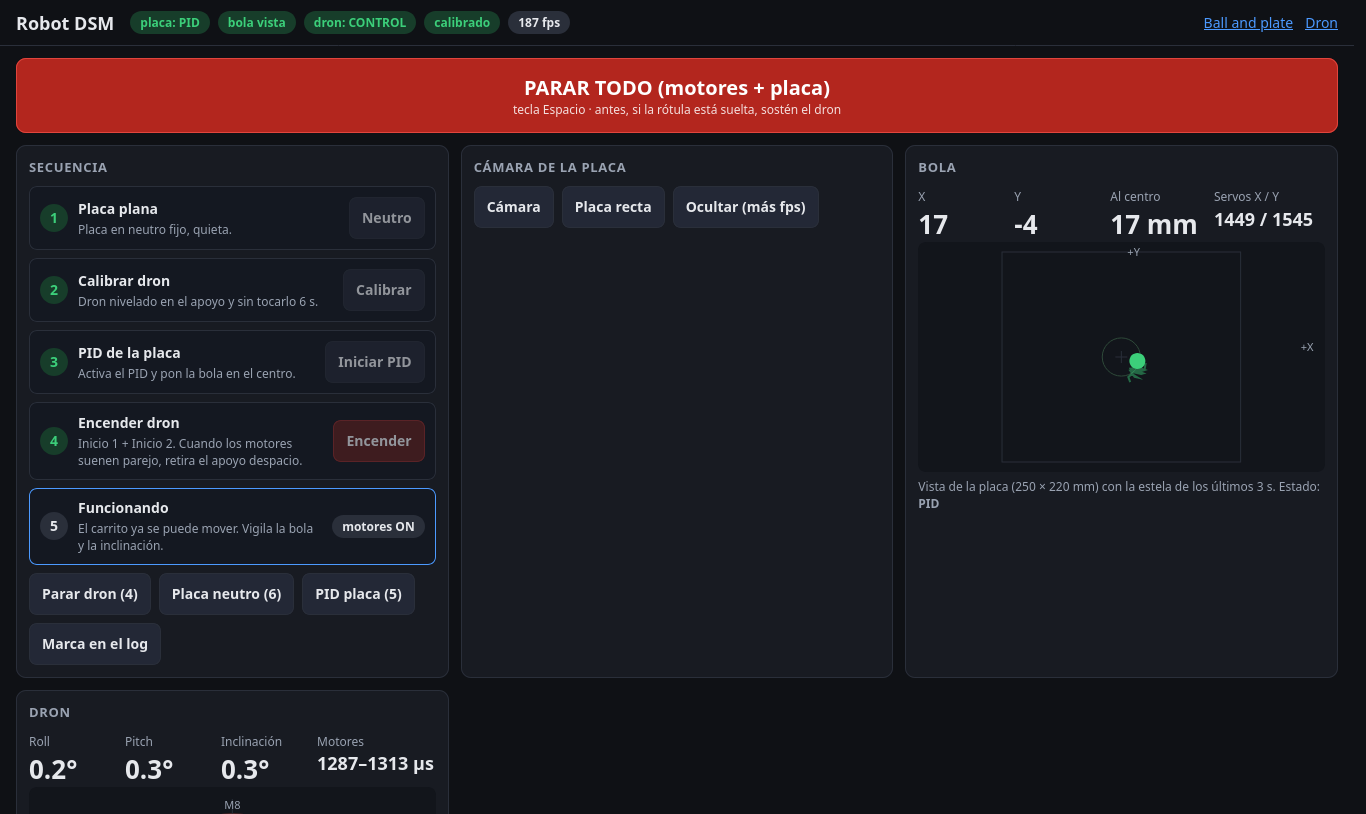
\includegraphics[width=\linewidth]{figures/ui_robot_page.png}\caption{\texttt{/robot} web page served by the Pi.}\end{subfigure}\hfill
  \begin{subfigure}[b]{0.45\textwidth}\centering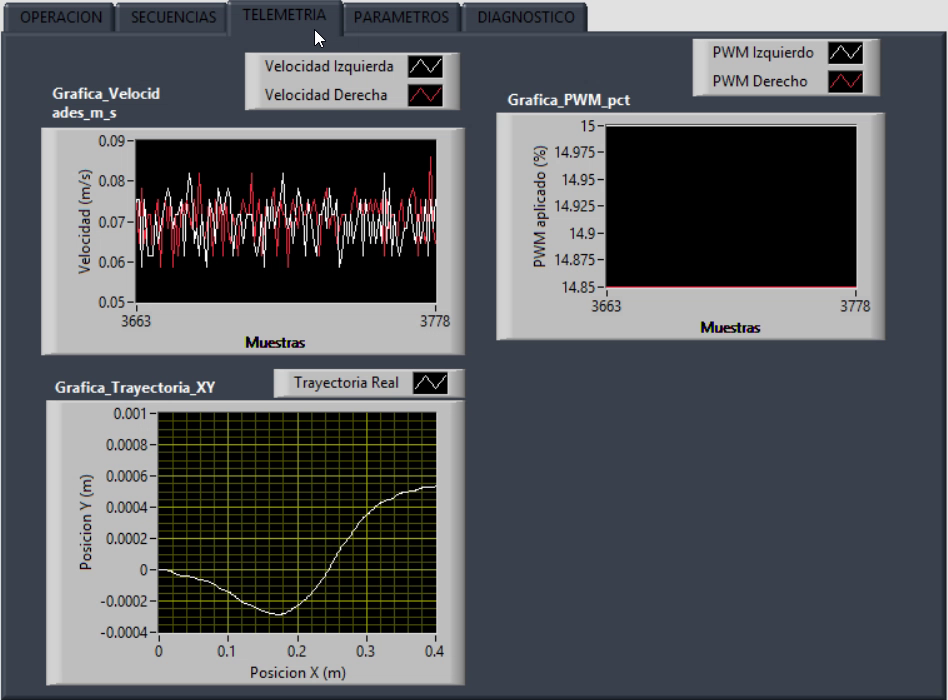
\includegraphics[width=\linewidth]{figures/ui_labview_telemetry.png}\caption{LabVIEW telemetry tab (myRIO).}\end{subfigure}
  \caption{Operator interfaces. The web page displays plate, ball, and drone status, a guided startup sequence, and a ``PARAR TODO'' (STOP ALL) button (also mapped to the spacebar); the LabVIEW panel shows wheel speeds, PWM, and the $x$--$y$ trajectory.}
  \label{fig:ui}
\end{figure}

\paragraph{Prerequisites}
\begin{itemize}
  \item charged batteries: both LiPo packs at \SI{12.6}{\volt} at rest and within \SI{0.05}{\volt} of each other, the NiMH pack, both 18650 packs, and the power bank;
  \item propellers inspected and tightened;
  \item vertical guide unobstructed, with both end-stops in place;
  \item a laptop or smartphone on the same Wi-Fi network as the Pi;
  \item two operators: one at the web page with the spacebar ready for immediate stop, and one watching the robot with the emergency stop (SB1) in hand;
  \item safety glasses for everyone within \SI{2}{\metre}.
\end{itemize}

\paragraph{Startup sequence}
Fig.~\ref{fig:fsm_dron} summarizes the octocopter firmware v11 state machine governing startup, guided flight, and safety cutoffs.
\begin{enumerate}
  \item With SB1 pressed, switch on logic power (SW1). \texttt{arrancar.sh} starts \texttt{seguidor.py} and restarts it if it exits. Wait for the NodeMCU to boot so the boot pulses emitted on GPIO5 and GPIO14 do not reach energized ESCs.
  \item Power on the myRIO and run the LabVIEW VI. The UART module must display the received ball position and drone angles (Fig.~\ref{fig:ui}b).
  \item On \texttt{/robot}:
  \begin{enumerate}[label=\alph*.]
    \item set the plate to ``Neutro'' (Neutral);
    \item with the drone level and still, click ``Calibrar'' (Calibrate) and wait \SI{5}{\second} until \texttt{CAL OK} appears;
    \item click ``Iniciar PID'' (Start PID) with the ball near the center.
  \end{enumerate}
  \item Measure and record the resting voltage of both LiPo packs, then connect them. Release SB1 (relays K1--K4 close). Click ``Armar e iniciar motores'' (Arm and start motors): the collective ramps up to \SI{1300}{\micro\second} (idle) and the attitude loop becomes active.
  \item \textbf{Bench mode} (moving base, drone at idle). Drive the base from LabVIEW using a manual command, a distance target, a \SI{360}{\degree} turn, go-to-point, or a loaded sequence.
  \item \textbf{Ramp mode} (proposed, Section~\ref{sec:porquedron}). Before the ramp, raise the collective with ``Subir'' (Up) to 1450--\SI{1550}{\micro\second} ($f\approx0.35$--0.55): the module remains seated while the rotors provide weight relief. Lower back to \SI{1300}{\micro\second} after clearing the climb. Above \SI{1500}{\micro\second}, the firmware limits the run to \SI{90}{\second}.
  \item \textbf{Guided flight.} Click ``Flotar'' (Hover): the collective ramps up at \SI{25}{\micro\second\per\second}, slowing to \SI{8}{\micro\second\per\second} above \SI{1650}{\micro\second}, up to \SI{1750}{\micro\second}. If the module does not lift off, click ``Subir'' ($+$\SI{25}{\micro\second}) and record the liftoff collective; if it exceeds \SI{1825}{\micro\second}, land and swap the batteries (Section~\ref{sec:bateria}). Use ``Subir''/``Bajar'' (Up/Down, $\pm$\SI{25}{\micro\second}) and ``Mantener'' (Hold); finish with ``Aterrizar'' (Land), which ramps down at \SI{60}{\micro\second\per\second}.
\end{enumerate}

\begin{figure}[!htbp]
\centering
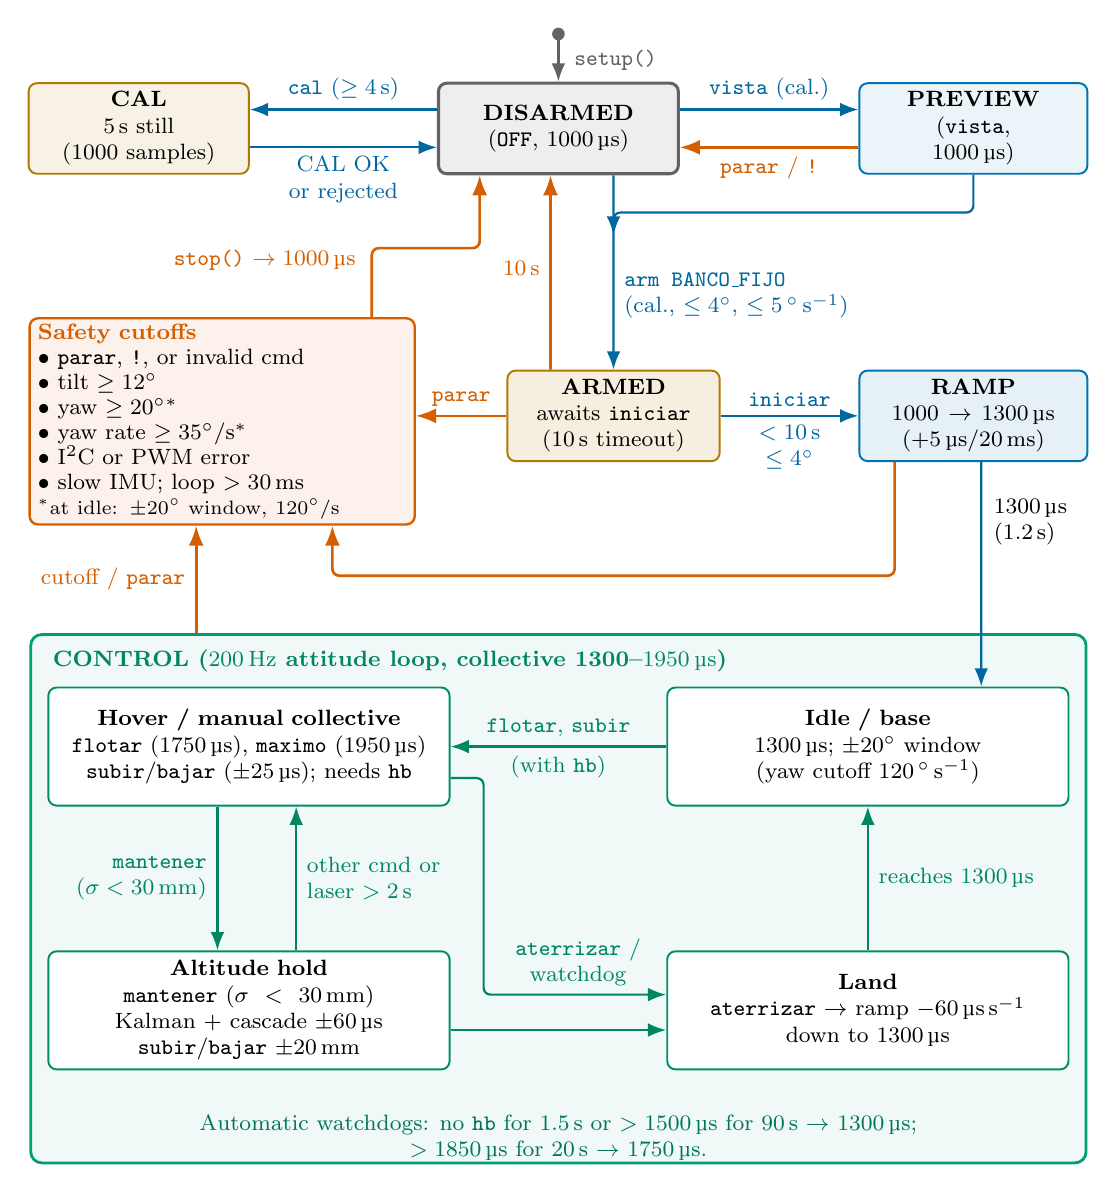
\begin{tikzpicture}[font=\footnotesize, >=Latex,
  st/.style={draw, rounded corners=3pt, align=center, minimum height=11.5mm, inner xsep=3.5pt, inner ysep=3pt, line width=0.7pt},
  stOff/.style={st, draw=pGris!90!black, fill=pGris!12, line width=1.1pt, text width=2.80cm},
  stPre/.style={st, draw=pOcre, fill=pOcre!10, text width=2.55cm},
  stVis/.style={st, draw=pAzul, fill=pAzul!8, text width=2.65cm},
  stArm/.style={st, draw=pOcre, fill=pOcre!12, text width=2.45cm},
  stRmp/.style={st, draw=pAzul, fill=pAzul!10, text width=2.65cm},
  stSub/.style={st, draw=pVerde!90!black, fill=white, minimum height=15mm, text width=4.85cm},
  stCut/.style={st, draw=pRojo, fill=pRojo!8, align=left, text width=4.68cm, line width=0.85pt, inner xsep=3pt, inner ysep=2pt, font=\footnotesize\linespread{0.95}\selectfont},
  tr/.style={->, line width=0.8pt, pAzul!90!black, rounded corners=2.5pt},
  trG/.style={->, line width=0.8pt, pVerde!85!black, rounded corners=2.5pt},
  trR/.style={->, line width=0.95pt, pRojo, rounded corners=2.5pt},
  lbl/.style={font=\footnotesize, align=center, inner sep=1.5pt}]

  % ---- Level 1: Preparation (y = 0.00, total width 0.00..13.50 cm <= 13.74 cm)
  \node[stPre] (cal) at (1.42, 0.00) {\textbf{CAL}\\ \SI{5}{\second} still\\ (1000 samples)};
  \node[stOff] (off) at (6.75, 0.00) {\textbf{DISARMED}\\ (\texttt{OFF}, \SI{1000}{\micro\second})};
  \node[stVis] (vis) at (12.02, 0.00) {\textbf{PREVIEW}\\ (\texttt{vista},\\ \SI{1000}{\micro\second})};

  % Start arrow into DISARMED
  \fill[pGris!90!black] (6.75, 1.20) circle (0.08);
  \draw[->, thick, pGris!90!black] (6.75, 1.13) -- node[right=2pt]{\texttt{setup()}} (off.north);

  % Level 1 transitions (gaps 2.85..5.20 = 2.35 cm and 8.30..10.55 = 2.25 cm)
  \draw[tr]  ([yshift=2.4mm]off.west) -- node[lbl, above=1.5pt]{\texttt{cal} ($\ge\SI{4}{\second}$)} ([yshift=2.4mm]cal.east);
  \draw[tr]  ([yshift=-2.4mm]cal.east) -- node[lbl, below=1.5pt]{CAL OK\\ or rejected} ([yshift=-2.4mm]off.west);
  \draw[tr]  ([yshift=2.4mm]off.east) -- node[lbl, above=1.5pt]{\texttt{vista} (cal.)} ([yshift=2.4mm]vis.west);
  \draw[trR] ([yshift=-2.4mm]vis.west) -- node[lbl, below=1.5pt, pRojo]{\texttt{parar} / \texttt{!}} ([yshift=-2.4mm]off.east);

  % ---- Level 2: Safety (left), ARMED (center), RAMP (right) (y = -3.65)
  \node[stCut] (cut) at (2.48, -3.72) {%
    \textbf{\textcolor{pRojo}{Safety cutoffs}}\\
    $\bullet$ \texttt{parar}, \texttt{!}, or invalid cmd\\
    $\bullet$ tilt $\ge\SI{12}{\degree}$\\
    $\bullet$ yaw $\ge20^\circ$$^\ast$\\
    $\bullet$ yaw rate $\ge35^\circ$/s$^\ast$\\
    $\bullet$ I$^2$C or PWM error\\
    $\bullet$ slow IMU; loop $>\SI{30}{\milli\second}$\\
    {\scriptsize $^\ast$at idle: $\pm20^\circ$ window, $120^\circ$/s}};
  \node[stArm] (arm) at (7.45, -3.65) {\textbf{ARMED}\\ awaits \texttt{iniciar}\\ (\SI{10}{\second} timeout)};
  \node[stRmp] (rmp) at (12.02, -3.65) {\textbf{RAMP}\\ $1000\to\SI{1300}{\micro\second}$\\ ($+5\us/\SI{20}{\milli\second}$)};

  % Level 1 <-> Level 2 transitions (vertical space -0.65..-2.55)
  % DISARMED and PREVIEW share the arm BANCO_FIJO transition into ARMED
  \draw[tr]  ([xshift=7mm]off.south) -- node[lbl, right=2pt, pos=0.62, align=left]{\texttt{arm BANCO\_FIJO}\\ (cal., $\le\SI{4}{\degree}$, $\le\SI{5}{\degree\per\second}$)} (arm.north);
  \draw[tr]  (vis.south) -- ++(0,-0.48) -| ([xshift=7mm]off.south |- 0,-1.35);
  % 10 s timeout from ARMED to DISARMED (left of arm.north)
  \draw[trR] ([xshift=-8mm]arm.north) -- node[lbl, left=2pt, pos=0.52, pRojo]{\SI{10}{\second}} ([xshift=-1mm]off.south);
  % Exit from Safety cutoffs to DISARMED (clean label above elbow, well above cut.north)
  \draw[trR] ([xshift=19mm]cut.north) -- (4.38,-1.52) -| ([xshift=-10mm]off.south);
  \node[lbl, pRojo, left=3pt, align=right] at (4.34, -1.68) {\texttt{stop()} $\to\SI{1000}{\micro\second}$};
  % Stop from ARMED to Safety cutoffs
  \draw[trR] (arm.west) -- node[lbl, above=1.5pt, pRojo]{\texttt{parar}} (cut.east |- arm.west);
  % ARMED -> RAMP (gap 8.80..10.55 = 1.75 cm)
  \draw[tr]  (arm.east) -- node[lbl, above=1.5pt]{\texttt{iniciar}} node[lbl, below=1.5pt, align=center]{$<\SI{10}{\second}$\\ $\le\SI{4}{\degree}$} (rmp.west);

  % ---- Level 3: CONTROL container (y = -6.30..-13.25, width 0.00..13.50 cm)
  \node[stSub] (flt) at (2.82, -7.85) {\textbf{Hover / manual collective}\\ \texttt{flotar} (\SI{1750}{\micro\second}), \texttt{maximo} (\SI{1950}{\micro\second})\\ \texttt{subir}/\texttt{bajar} ($\pm\SI{25}{\micro\second}$); needs \texttt{hb}};
  \node[stSub] (ral) at (10.68, -7.85) {\textbf{Idle / base}\\ \SI{1300}{\micro\second}; $\pm\SI{20}{\degree}$ window\\ (yaw cutoff \SI{120}{\degree\per\second})};
  \node[stSub] (alt) at (2.82, -11.20) {\textbf{Altitude hold}\\ \texttt{mantener} ($\sigma<\SI{30}{\milli\metre}$)\\ Kalman + cascade $\pm\SI{60}{\micro\second}$\\ \texttt{subir}/\texttt{bajar} $\pm\SI{20}{\milli\metre}$};
  \node[stSub] (atr) at (10.68, -11.20) {\textbf{Land}\\ \texttt{aterrizar} $\to$ ramp $-\SI{60}{\micro\second\per\second}$\\ down to \SI{1300}{\micro\second}};

  % Automatic watchdogs note inside CONTROL (centered without forced justification)
  \node[font=\footnotesize, text=pVerde!75!black, align=center] (vig) at (6.75, -12.82)
    {Automatic watchdogs: no \texttt{hb} for \SI{1.5}{\second} or $>\SI{1500}{\micro\second}$ for \SI{90}{\second} $\to$ \SI{1300}{\micro\second};\\
     $>\SI{1850}{\micro\second}$ for \SI{20}{\second} $\to$ \SI{1750}{\micro\second}.};

  % CONTROL container frame on background layer
  \begin{scope}[on background layer]
    \node[draw=pVerde, fill=pVerde!6, rounded corners=4pt, line width=1pt,
          fit=(flt)(ral)(alt)(atr)(vig), inner xsep=6pt, inner ysep=8pt,
          yshift=3.8mm] (ctrl) {};
  \end{scope}
  \node[font=\footnotesize\bfseries, text=pVerde!85!black, anchor=north west]
    at ([xshift=5pt, yshift=-2.5pt]ctrl.north west) {CONTROL (\SI{200}{\hertz} attitude loop, collective 1300--\SI{1950}{\micro\second})};

  % RAMP -> CONTROL (Idle) entry (label to the right of the blue arrow, clear of the red arrow)
  \draw[tr] ([xshift=1mm]rmp.south) -- (ral.north -| 12.12,0);
  \node[lbl, right=2pt, align=left] at (12.15, -5.00) {\SI{1300}{\micro\second}\\ (\SI{1.2}{\second})};

  % Internal transitions inside CONTROL (ample vertical space -8.70..-10.35)
  \draw[trG] (ral.west) -- node[lbl, above=1.5pt]{\texttt{flotar}, \texttt{subir}} node[lbl, below=1.5pt]{(with \texttt{hb})} (flt.east);
  \draw[trG] ([xshift=-4mm]flt.south) -- node[lbl, left=2pt, align=right]{\texttt{mantener}\\ ($\sigma<\SI{30}{\milli\metre}$)} ([xshift=-4mm]alt.north);
  \draw[trG] ([xshift=6mm]alt.north) -- node[lbl, right=2pt, align=left]{other cmd or\\ laser $>\SI{2}{\second}$} ([xshift=6mm]flt.south);
  \draw[trG] ([yshift=-4mm]flt.east) -- (5.80,-8.25) |- ([yshift=2mm]atr.west);
  \node[lbl, text=pVerde!85!black, above=1.5pt, align=center] at (7.00,-11.00) {\texttt{aterrizar} /\\ watchdog};
  \draw[trG] ([yshift=-2.5mm]alt.east) -- ([yshift=-2.5mm]atr.west);
  \draw[trG] (atr.north) -- node[lbl, right=2pt]{reaches \SI{1300}{\micro\second}} (ral.south);

  % Safety exits from RAMP and CONTROL to Safety cutoffs (in open corridor -5.65)
  \draw[trR] ([xshift=-10mm]rmp.south) -- (11.02,-5.68) -| ([xshift=14mm]cut.south);
  \draw[trR] (ctrl.north -| 2.15,0) -- node[lbl, left=2pt, pRojo]{cutoff / \texttt{parar}} (cut.south -| 2.15,0);
\end{tikzpicture}
\vspace{-4pt}
\caption{\raggedright Octocopter firmware v11 state machine (\texttt{captura\_octo\_m8\_vuelo\_guia.ino}). Transition functions: boot to \texttt{DISARMED} (\texttt{setup()}); serial commands \texttt{cal}, \texttt{vista}, \texttt{arm BANCO\_FIJO}, \texttt{iniciar}, \texttt{flotar}, \texttt{maximo}, \texttt{subir}, \texttt{bajar}, \texttt{mantener}, \texttt{aterrizar}, \texttt{parar}, and rejected command (\texttt{command()}); \texttt{!} stop and invalid line (\texttt{serialInput()}); calibration end (\texttt{collectCalibration()}); \SI{10}{\second} timeout in \texttt{ARMED}, \texttt{RAMP} to \texttt{CONTROL} (\SI{1300}{\micro\second}), and MCPWM fault (\texttt{loop()}); collective and \texttt{hb} heartbeat (\texttt{fijarObjetivo()}, \texttt{hbReciente()}); collective ramp, altitude hold, and watchdogs (\SI{1.5}{\second}, \SI{20}{\second}, \SI{90}{\second}, and \SI{2}{\second} without laser; \texttt{actualizarColectivo()}); attitude/yaw cutoffs (\texttt{checkAttitudeCutoff()}); and I$^2$C error, IMU $>\SI{15}{\milli\second}$, or late loop (\texttt{imuFault()} from \texttt{loop()}). Every cutoff calls \texttt{stop()} (\SI{1000}{\micro\second}, \texttt{DISARMED}).}
\label{fig:fsm_dron}
\end{figure}

\paragraph{Reading results}
Each run produces three logs:
\begin{itemize}
  \item \texttt{registros/registro\_*.csv}: ball position, servo pulses, and status at the camera frame rate;
  \item \texttt{registros/vuelo\_*.csv}: drone attitude, motor commands, accelerometer, laser range, and collective at \SI{10}{\hertz};
  \item the drone onboard buffer (last \SI{16}{\second} at \SI{100}{\hertz}, 1600 samples), exported via ``Exportar registro'' (Export log).
\end{itemize}
The scripts in \texttt{analysis/} compute the metrics reported in Section~\ref{sec:validation}. Record the resting LiPo voltage before and \SI{10}{\minute} after each flight, along with each video timestamp, so videos can be cross-referenced with the logs as in Section~\ref{sec:flights}.

\paragraph{Operating limits and protections}
Drone firmware v11 stops the motors in five cases:
\begin{itemize}
  \item estimated tilt exceeds \SI{12}{\degree};
  \item above \SI{1400}{\micro\second} (or with base yaw rate \texttt{yb} active), relative yaw exceeds \SI{20}{\degree} or relative yaw rate exceeds \SI{35}{\degree\per\second};
  \item at idle on the base ($\le\SI{1400}{\micro\second}$, without \texttt{yb}), the heading reference slides within a $\pm\SI{20}{\degree}$ window without angle cutoff, while a \SI{120}{\degree\per\second} rate cutoff remains active;
  \item the estimated IMU state becomes non-finite;
  \item any unknown command arrives.
\end{itemize}
It also limits the collective in three situations:
\begin{itemize}
  \item without the Pi heartbeat (\texttt{hb}, sent every \SI{0.3}{\second}), the collective is capped at \SI{1400}{\micro\second}, and after \SI{1.5}{\second} without a heartbeat it drops to \SI{1300}{\micro\second};
  \item above \SI{1850}{\micro\second}, the collective returns to \SI{1750}{\micro\second} after \SI{20}{\second} to protect the \SI{30}{\ampere} fuses;
  \item above \SI{1500}{\micro\second}, the collective drops after \SI{90}{\second}.
\end{itemize}
The firmware does not measure battery voltage. With charged LiPo packs, useful continuous hover time is 3--\SI{7}{\minute} (Section~\ref{sec:bateria}); keep runs short and do not discharge LiPo packs below \SI{11.1}{\volt} at rest (\SI{3.7}{\volt} per cell).

\paragraph{Safe shutdown}
\begin{enumerate}
  \item Click ``Aterrizar'' (Land) and wait for the collective to reach \SI{1300}{\micro\second}; then click ``Parar'' (Stop).
  \item Set the plate to ``Neutro'' (Neutral) and stop the base.
  \item Press SB1 and disconnect the LiPo batteries before touching the drone.
  \item Export the logs and record the resting LiPo voltage.
\end{enumerate}
In an emergency, press the spacebar (all motors stop immediately and the drone drops onto the lower end-stop) and press the emergency stop (SB1), which simultaneously disconnects both LiPo branches, the mobile base, and the servos.

\subsection{Basic troubleshooting}
\label{sec:troubleshooting}
Table~\ref{tab:troubleshooting} summarizes faults observed during prototype testing, their probable causes, and recommended actions.

\begin{table}[!htbp]
\centering
\caption{Basic troubleshooting for faults observed during AeroTray operation.}
\label{tab:troubleshooting}
\footnotesize
\begin{tabularx}{\textwidth}{@{}>{\raggedright\arraybackslash}p{0.27\textwidth}>{\raggedright\arraybackslash}p{0.31\textwidth}>{\raggedright\arraybackslash}X@{}}
\toprule
Symptom & Probable cause & Recommended action \\
\midrule
\texttt{ORDEN RECHAZADA} or \texttt{CAL RECHAZADA} when calibrating & IMU did not initialize after flashing or rebooting the NodeMCU (\texttt{IMU=0} at boot) & Press EN on the NodeMCU, wait \SI{5}{\second}, and calibrate with the drone still and level \\
Web page unresponsive or Pi not visible & Laptop or Pi switched networks & Connect both to the same hotspot and locate the Pi by its MAC address \\
Servos receive pulses but the plate does not move & Missing servo power (BT6, regulator, or common ground) & Check BT6, the XL4015 at \SI{5.2}{\volt}, and the common ground with the ESP32-S3 \\
Laser reports \texttt{estado 2} or invalid readings & Weak return signal from the floor & Place the white target sheet under the sensor; the firmware uses long-range mode with filtering \\
Ball is not detected & Lighting or color & Control ambient lighting; inspect the ``Cámara'' (Camera) view on \texttt{/robot} \\
\texttt{Flotar} does not lift off & Discharged LiPo packs ($<\SI{12.4}{\volt}$ at rest) & Measure and charge the LiPo packs; at \SI{11.1}{\volt} the module cannot lift off below the sustained limit \\
Tilt (\SI{12}{\degree}) or yaw cutoff & Impact at a ramp break or base rotation with collective $>\SI{1400}{\micro\second}$ & Recalibrate and re-arm; cross the ramp at idle \\
\bottomrule
\end{tabularx}
\end{table}
           % 7. Operation instructions
%% ======================================================================
%% 09_validation.tex -- 8. Validation and characterization (+ model validation)
%% ======================================================================
\section{Validation and characterization}
\label{sec:validation}

Validation follows the scenarios defined in the course guide: mobile-base motion on flat ground and on a \SI{10}{\degree} slope, ball balancing with the base stationary and moving, and stability of the intermediate stage (the octocopter). All results come from logs recorded on November 17, 18, 20, and 23, 2026, and published in the repository. Ball error is the Euclidean distance between the ball and the plate center (reference $(0,0)$), computed only while the PID controller was active and the ball was detected.

\subsection{Test methodology and metrics}
\label{sec:metodologia}
The final test protocol (Nov.~23) defined configurations that add \emph{one element at a time}, isolating each error increase to the newly added subsystem:
\begin{itemize}
  \item C0: unpowered measurements (\emph{completed});
  \item C1: ball and plate alone, with the base stationary and the drone off (\emph{completed});
  \item C2: moving base with the drone locked to the base, equivalent to a \emph{servos-only} solution (\emph{pending});
  \item C3: full robot with the drone free on the spherical joint (\emph{completed}).
\end{itemize}
The protocol also includes test~D (comparing C2 and C3 over the same ramp cycle as a direct test of Section~\ref{sec:porquedron}), as well as dedicated tape-measured translation/rotation tests (E1), a sinusoidal plate sweep (E2), recovery from 2 and \SI{5}{\centi\metre} offsets (E3), and weight relief at $f=0.5$. These tests were not executed during the Nov.~23 campaign and remain future work (Section~\ref{sec:limits}). Table~\ref{tab:metricas} summarizes the metrics defined in \texttt{metricas\_pruebas.py} and their measurement status.

\begin{table}[!htbp]
\centering
\small
\caption{Performance metrics, acceptance criteria, and validation status. $e(t)$ is the ball distance to the center, in mm, while the PID is active; $R_u=\SI{96.5}{\milli\metre}$ is the usable plate radius.}
\label{tab:metricas}
\begin{tabularx}{\textwidth}{@{}>{\raggedright\arraybackslash}p{0.23\textwidth}>{\raggedright\arraybackslash}X>{\raggedright\arraybackslash}p{0.22\textwidth}>{\raggedright\arraybackslash}p{0.15\textwidth}@{}}
\toprule
Metric & Definition & Criterion & Status \\
\midrule
Relative error & $e_{\mathrm{RMS}}/R_u\times100$ & E3: $\le\SI{10}{\percent}$ (off), $\le\SI{30}{\percent}$ (idle); E4/E5: $\le\SI{45}{\percent}$ & measured (Table~\ref{tab:ensayos23}) \\
Effectiveness & \% of time with $e\le\SI{30}{\milli\metre}$ (and \SI{50}{\milli\metre} band on Nov.~23) & E3: $\ge\SI{90}{\percent}$; E4/E5: $\ge\SI{60}{\percent}$ & measured (Tables~\ref{tab:ensayos23}--\ref{tab:completos23}) \\
Ball losses and success rate & intervals $>\SI{1}{\second}$ without ball; loss-free / total trials & $\ge\SI{80}{\percent}$ & measured on bench and ramp \\
Recovery (2 and \SI{5}{\centi\metre}) & time to enter band (5 or \SI{20}{\milli\metre}) and stay \SI{2}{\second}; overshoot & $\le$3 and \SI{5}{\second}; success $\ge\SI{80}{\percent}$ & pending (E3) \\
Servo control effort & $\sqrt{\overline{(u_x-n_x)^2+(u_y-n_y)^2}}$ (\si{\micro\second}); activity $\sum|\Delta u|/T$ & compare C1, C2, and C3, and D-A vs.\ D-B & C1/C3 measured; C2 and D pending \\
Servo usage and saturation & mean $\max|u-n|/\SI{220}{\micro\second}$; \% of time $\ge\SI{95}{\percent}$ & saturation $\le\SI{10}{\percent}$ & measured (Nov.~18 and Pi Nov.~23) \\
Drone control effort & spread across the 8 motors (\si{\micro\second}) and mean collective & zero cutoffs in base mode & measured (Secs.~\ref{sec:flights}--\ref{sec:ensayos23}) \\
Base: translation and rotation & $|d-d_{\mathrm{ref}}|/d_{\mathrm{ref}}$ and $|\psi-\SI{360}{\degree}|/\SI{360}{\degree}$ & $\le\SI{5}{\percent}$ & speed and drift measured; 25/50\,cm and \SI{360}{\degree} pending \\
Platform & max frequency with amplitude $\ge\SI{70}{\percent}$ (0.5--\SI{4}{\hertz} sweep) & $\ge\SI{1}{\hertz}$ & pending (E2) \\
\bottomrule
\end{tabularx}
\end{table}

\paragraph{Unpowered measurements (C0, Nov.~23)} These measurements replaced values that the model previously took from CAD or estimates:
\begin{itemize}
  \item total robot mass: \SI{10.4}{\kilo\gram};
  \item wheelbase: \SI{0.22}{\metre};
  \item vertical guide travel: roughly \SI{140}{\milli\metre} (CAD indicated \SI{77}{\milli\metre});
  \item static tip-over angles: \SI{21.5}{\degree} and \SI{30.5}{\degree}, yielding $x_G=\SI{88}{\milli\metre}$ and $h_G=\SI{224}{\milli\metre}$;
  \item spherical joint range: \SI{35}{\degree} toward M8, \SI{40}{\degree} toward M6, \SI{47}{\degree} toward M5, and \SI{53}{\degree} toward M7.
\end{itemize}
The spherical joint range comfortably exceeds the \SI{10}{\degree} base angle change at each ramp transition. Therefore, the Nov.~18 tilt cutoffs upon entering the ramp did not result from the module hitting a mechanical stop. Instead, dynamics explain them: the transition impact excites an inverted pendulum that has low torque authority at idle.

\subsection{Octocopter on the bench (rotors at idle)}
On Nov.~18, the drone operated at a fixed \SI{1300}{\micro\second} collective on the free spherical joint while pushed by hand. The onboard buffer logged data at 190--\SI{200}{\hertz} (Fig.~\ref{fig:bench}).

\begin{itemize}
  \item Across both trials, RMS roll was \SI{0.38}{\degree} and \SI{0.26}{\degree}, and RMS pitch was \SI{0.26}{\degree} and \SI{0.24}{\degree}.
  \item Maximum tilt was \SI{1.42}{\degree}.
  \item Motor commands stayed between \SI{1255}{\micro\second} and \SI{1338}{\micro\second}, indicating low control effort.
  \item After the largest push (\SI{3.7}{\degree}), the drone re-leveled in about \SI{1}{\second}.
\end{itemize}

\begin{figure}[!htbp]
  \centering
  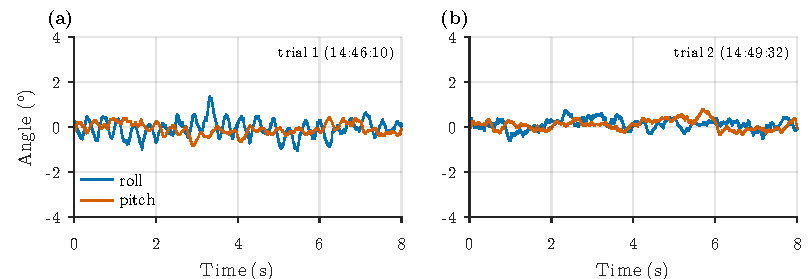
\includegraphics{figures/fig_drone_bench.pdf}
  \caption{Octocopter attitude on the free spherical joint at idle collective (\SI{1300}{\micro\second}), logged onboard at 190--\SI{200}{\hertz}.}
  \label{fig:bench}
\end{figure}

\subsection{Flight campaign on the vertical guide}
\label{sec:flights}
On Nov.~20, nine flights were performed on the vertical guide across successive firmware versions, starting the afternoon session with the LiPo batteries charged to 12.4\,V at rest. Table~\ref{tab:flights} and Fig.~\ref{fig:flights} summarize the campaign.

\begin{itemize}
  \item \textbf{Flights 1--2.} Revealed two issues: accelerometer saturation from rotor vibration (\SIrange{0.03}{2.2}{g}), which triggered false tilt cutoffs, and real yaw rotation of the drone on the spherical joint. These findings led to the \SI{10}{\hertz} accelerometer filter and the yaw loop.
  \item \textbf{Flights 3--6.} Lifted off, then slowly drifted in pitch or roll until the operator or safety interlock stopped them. The drift had a 5--\SI{10}{\second} period and was identical with full gains (v5) and reduced gains (v6). This pointed to the torque-authority limit of Section~\ref{sec:authority}---whose region of attraction was only 3--4$^\circ$---rather than gain tuning.
  \item \textbf{Flight 7} (v8, wider angular-rate limit). First stable hover: \SI{20}{\second} at 1725--\SI{1775}{\micro\second}, with \SI{0.55}{\degree} RMS roll and \SI{1.19}{\degree} RMS pitch. A cutoff occurred during landing when gains reverted to bench values while the drone was still airborne.
  \item \textbf{Flights 8--9} (v9, with hysteresis). Flew and landed without cutoff. In Flight~9, takeoff required \SI{1796}{\micro\second} (\SI{21}{\micro\second} higher than Flight~8) and collective was raised to \SI{1816}{\micro\second}; after \SI{48}{\second} of hovering, pitch diverged to the \SI{12}{\degree} limit. Allocation saturation does not explain this, because \eqref{eq:taumax} still provides \SI{2.4}{\newton\metre}. The candidate causes are the lightly damped slow mode of Section~\ref{sec:attitude}, whose damping depends on $k_T$, and battery voltage sag, which reduces $k_T$ with $V_{\mathrm{bus}}^2$: by the end of Flight~9, each LiPo had delivered \SI{1.0}{\ampere\hour} that afternoon (Section~\ref{sec:bateria}). Later, at 11.1\,V, the module no longer lifted off.
\end{itemize}

\begin{table}[!htbp]
\centering
\caption{Flight campaign on the vertical guide (November 20, 2026). RMS error relative to horizontal, computed while mean motor command exceeded \SI{1650}{\micro\second}.}
\label{tab:flights}
\footnotesize
\setlength{\tabcolsep}{4pt}
\begin{tabularx}{\textwidth}{@{}clrrrrr>{\raggedright\arraybackslash}X@{}}
\toprule
Flight & FW & Max.\ col. & $t$ & Roll & Pitch & Max. & Outcome \\
 & & (\si{\micro\second}) & (\si{\second}) & RMS (\si{\degree}) & RMS (\si{\degree}) & tilt (\si{\degree}) & \\
\midrule
1 & v2 & 1625 & 0 & -- & -- & -- & tilt cutoff (accelerometer vibration) \\
2 & v3 & 1475 & 0 & -- & -- & -- & yaw cutoff ($-20^\circ$) \\
3 & v4 & 1700 & 10.9 & 0.93 & 4.89 & 9.8 & operator stop, pitch drift \\
4 & v5 & 1800 & 19.4 & 2.99 & 0.95 & 9.3 & operator stop, slow oscillation \\
5 & v6 & 1700 & 3.1 & 0.83 & 3.59 & 10.9 & tilt cutoff at takeoff \\
6 & v6 & 1725 & 8.4 & 4.14 & 1.38 & 11.1 & roll cutoff (videos IMG\_1867--1868) \\
7 & v8 & 1775 & 27.2 & 0.55 & 1.19 & 4.3 & \SI{20}{\second} hover; cutoff on landing (video IMG\_1869) \\
8 & v9 & 1775 & 31.0 & 1.15 & 0.95 & 3.8 & hover and landing, no cutoff \\
9 & v9 & 1816 & 62.0 & 1.73 & 1.70 & 10.8 & \SI{48}{\second} hover; pitch cutoff \\
\bottomrule
\end{tabularx}
\end{table}

\begin{figure}[!htbp]
  \centering
  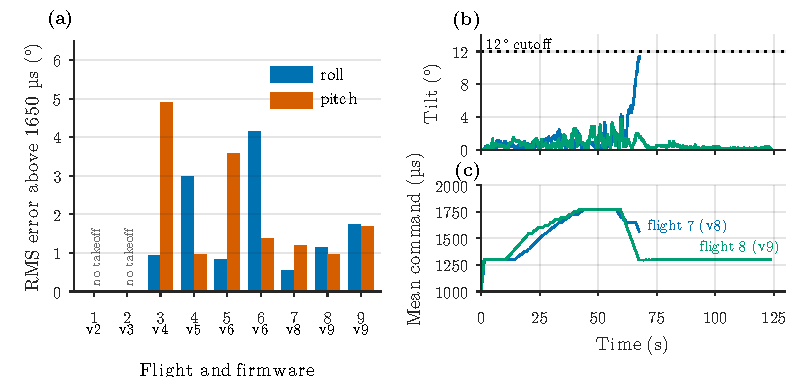
\includegraphics{figures/fig_flight_campaign.pdf}
  \caption{Flight campaign on the vertical guide. (a) RMS roll and pitch error above \SI{1650}{\micro\second} for each flight, with firmware version. (b) Tilt and (c) mean motor command for Flights~7 (v8) and 8 (v9): v8 cuts off when flight gains deactivate during landing, whereas v9 lands normally.}
  \label{fig:flights}
\end{figure}

\paragraph{Videos synchronized with telemetry}
The three Nov.~20 videos (iPhone, 4K at \SI{120}{fps}) were synchronized with the logs using the file creation timestamp (which marks recording start on iPhone) and the PC timestamp on each log line (Fig.~\ref{fig:video}). IMG\_1867 (15:10:11, \SI{11}{\second}) shows Flight~6 as the collective ramps from 1600 to \SI{1675}{\micro\second}. IMG\_1868 (15:10:26, \SI{4}{\second}) captures its end: roll moves from $-6^\circ$ to $-11.1^\circ$ in \SI{1.3}{\second}, the firmware cuts the motors, and the module drops onto the guide, matching the log within \SI{1}{\second}. IMG\_1869 (15:23:32, \SI{13}{\second}) falls inside the Flight~7 hover, with collective between 1763 and \SI{1775}{\micro\second} and tilt between 0.1 and 1.7$^\circ$. In all three videos, an operator follows the camera mast by hand as a safety measure; the footage cannot rule out light contact, which would act as an additional disturbance on the attitude loop; the figures in Table~\ref{tab:flights} are reported directly from the logs.

\begin{figure}[!htbp]
  \centering
  \begin{subfigure}[b]{0.24\textwidth}\centering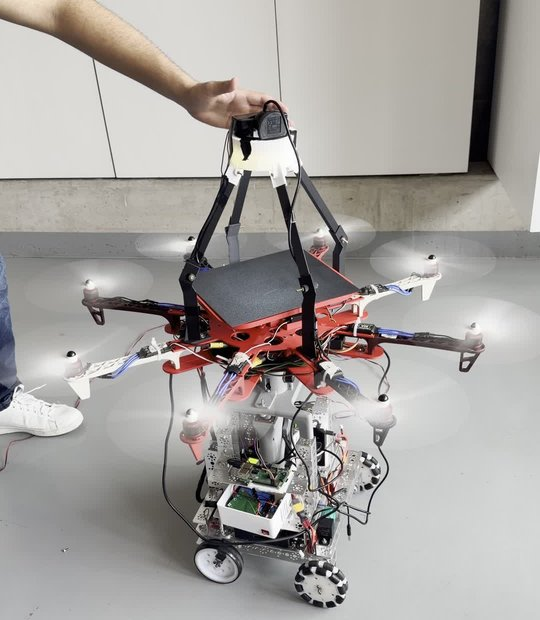
\includegraphics[width=\linewidth]{figures/video_a.jpg}\caption{Flight~6, \SI{1650}{\micro\second}.}\end{subfigure}\hfill
  \begin{subfigure}[b]{0.24\textwidth}\centering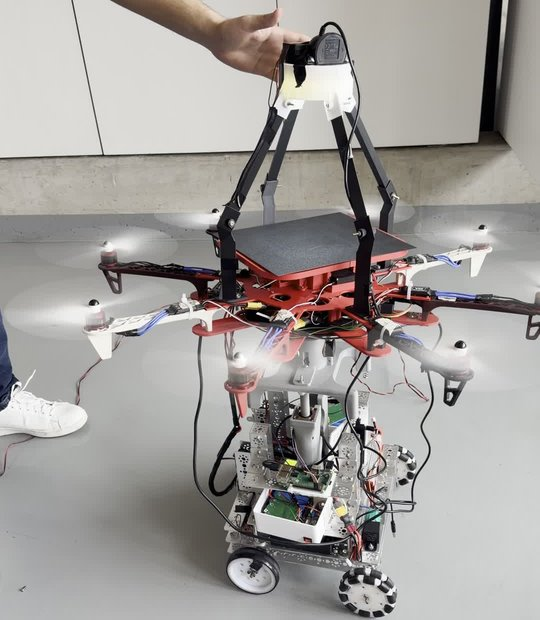
\includegraphics[width=\linewidth]{figures/video_b.jpg}\caption{Flight~6, \SI{1724}{\micro\second}.}\end{subfigure}\hfill
  \begin{subfigure}[b]{0.24\textwidth}\centering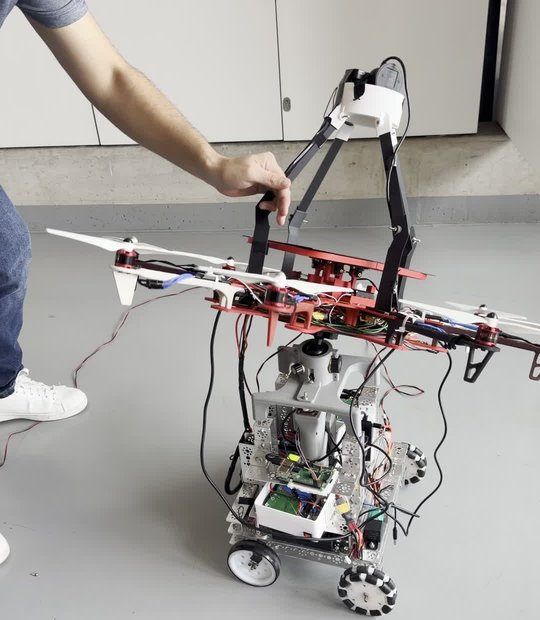
\includegraphics[width=\linewidth]{figures/video_c.jpg}\caption{Flight~6, after cutoff.}\end{subfigure}\hfill
  \begin{subfigure}[b]{0.24\textwidth}\centering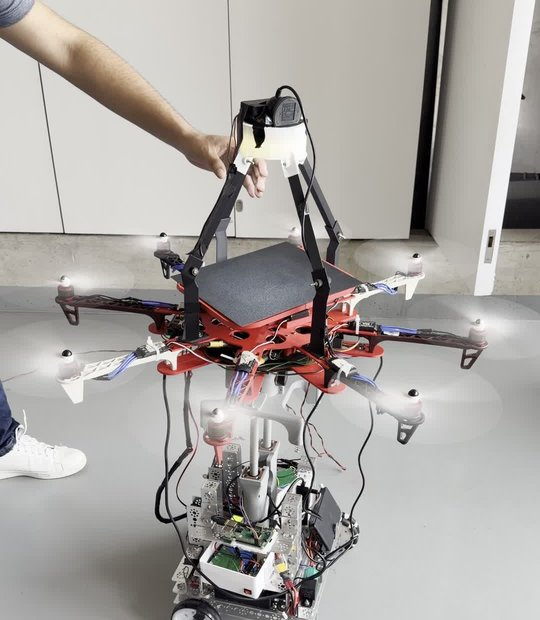
\includegraphics[width=\linewidth]{figures/video_d.jpg}\caption{Flight~7, \SI{1774}{\micro\second}.}\end{subfigure}
  \caption{Frames from the Nov.~20 videos synchronized with telemetry: (a) IMG\_1867 at \SI{6}{\second}, (b) IMG\_1868 at \SI{1}{\second}, (c) IMG\_1868 at \SI{3.2}{\second}, after the $-11.1^\circ$ roll cutoff with motors stopped and the module resting on its side, and (d) IMG\_1869 at \SI{7}{\second}, hovering at 0.4--0.6$^\circ$ tilt. The LiPo batteries were near 12.4\,V.}
  \label{fig:video}
\end{figure}

\paragraph{Comparison with the Isaac Lab model}
Before testing, the assembly was modeled in Isaac Lab \cite{mittal2023} from CAD, including the spherical joint and vertical guide (\SI{3.6}{\kilo\gram}, thrust capped at \SI{6}{\newton} per motor). Both a PPO policy \cite{schulman2017} and a classical PI-D controller were trained and evaluated there. Comparison yields two distinct findings:
\begin{itemize}
  \item \textbf{Thrust.} The model predicted hover at \SI{1899}{\micro\second} (\SI{4.41}{\newton} per motor); the physical assembly lifted off 124--\SI{174}{\micro\second} earlier, meaning the actual thrust gain is 33--52\% higher (Section~\ref{sec:ident}). The thrust model was conservative, and that error---not controller tuning---placed the physical attitude loop inside the stable region of Fig.~\ref{fig:dronestab}b. The simulator also omitted battery voltage, which shifts takeoff by more than \SI{100}{\micro\second} on the prototype between full charge and discharge (Section~\ref{sec:bateria}).
  \item \textbf{Attitude.} Simulated RMS tilt was \SI{0.02}{\degree} with PPO, \SI{0.04}{\degree} with the classical controller, and \SI{0.12}{\degree} under disturbances; measured values are 0.55--\SI{1.7}{\degree}. The model ignored four effects that dominated hardware behavior: rotor vibration on the IMU, center-of-mass eccentricity (\SI{9.5}{\milli\metre}), angular-rate command saturation, and the loop delay and actuation lag that, combined with the inverted-pendulum pole, push the loop near the limit of Section~\ref{sec:limits_fund}. All eight simulated motors were symmetric, whereas the measured median spread across motors was 50--\SI{90}{\micro\second}.
\end{itemize}

\subsection{Ball and plate with the base stationary and moving}
Fig.~\ref{fig:bp} and Table~\ref{tab:bp} compare four conditions:
\begin{enumerate}[label=(\alph*)]
  \item stationary base with the drone off (Nov.~17, \SI{75}{\second});
  \item stationary base with all eight rotors at idle and the attitude loop active (Nov.~17, \SI{469}{\second});
  \item robot driving straight and turning on flat ground (Nov.~18, four runs, \SI{582}{\second});
  \item robot climbing and descending the \SI{10}{\degree} ramp (Nov.~18, six runs, \SI{345}{\second}).
\end{enumerate}
Each run in (c) and (d) was matched to its video via the video file timestamp.

\begin{table}[!htbp]
\centering
\caption{Ball error $|e|$ (distance to plate center, in mm) across the four conditions. Ball diameter \SI{27}{\milli\metre}; plate half-width \SI{110}{\milli\metre}.}
\label{tab:bp}
\small
\begin{tabular}{@{}lrrrrr@{}}
\toprule
Condition & Samples & Median & Mean & P90 & P95 \\
\midrule
(a) stationary base, drone off & 13\,951 & 4.4 & 4.4 & 4.4 & 4.5 \\
(b) stationary base, drone at idle & 85\,219 & 18.9 & 23.1 & 39.9 & 60.4 \\
(c) moving, flat ground & 95\,851 & 27.9 & 33.1 & 63.2 & 76.2 \\
(d) moving, \SI{10}{\degree} ramp & 62\,492 & 29.5 & 35.8 & 63.9 & 87.9 \\
\bottomrule
\end{tabular}
\end{table}

\begin{figure}[!htbp]
  \centering
  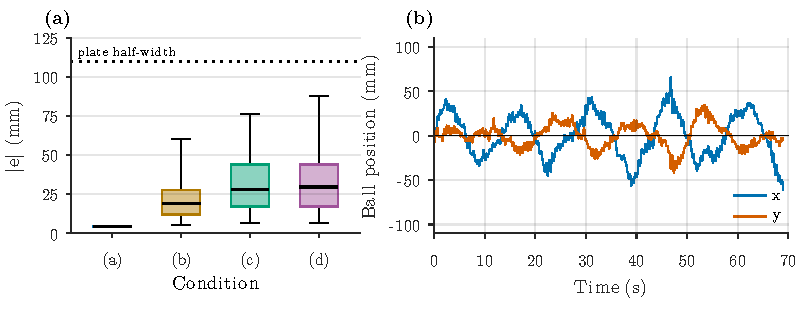
\includegraphics[width=\textwidth]{figures/fig_bp_results.pdf}
  \caption{Left: ball error distribution for conditions (a)--(d) of Table~\ref{tab:bp} (box: quartiles; whiskers: 5th and 95th percentiles). Right: ball position during a ramp run (video \texttt{VID\_20261118\_165747}).}
  \label{fig:bp}
\end{figure}

\paragraph{Discussion}
\begin{itemize}
  \item \textbf{Drone off.} With the drone off, the error is constant at \SI{4.4}{\milli\metre}: the ball settles inside the servo deadband. Vision noise lies well below this level.
  \item \textbf{Rotors at idle.} Turning the rotors on quadruples the median error (to \SI{18.9}{\milli\metre}). The propagation model shows that residual octocopter attitude (within \SI{0.4}{\degree}) accounts for only about \SI{2}{\milli\metre} RMS; the remainder is a slow load acting directly on the ball (rotor downwash, vibration, and backlash), concentrated below \SI{0.3}{\hertz} (Section~\ref{sec:coupling}). With the earlier gains ($k_i=0.2$), the ball fell off in under \SI{5}{\second}; after increasing the integral gain to 0.8, no drops occurred in a \SI{20}{\second} check, and the \SI{469}{\second} trial of condition~(b) completed without drops.
  \item \textbf{Moving base.} Moving the base adds roughly \SI{10}{\milli\metre} to the median and widens the tail (P95 of 76--\SI{88}{\milli\metre}), consistent with the spherical-joint acceleration term in \eqref{eq:balllinx} and its amplification through the octocopter (Fig.~\ref{fig:transm}c). Ramp performance is only slightly worse than flat ground: as \eqref{eq:tilt} predicts, the spherical joint absorbs the \SI{10}{\degree} slope and the octocopter keeps the plate level. With the tray fixed to the base, that same slope would have left the servos only \SI{0.8}{\degree} of usable travel (Section~\ref{sec:porquedron}).
  \item \textbf{Ball detection.} During moving-base runs, the ball was detected 61--100\% of the time. Gaps include drops off the plate edge---often at the ramp transitions, where the accelerometer recorded impacts up to \SI{1.95}{g}---and intervals while the ball was replaced by hand.
\end{itemize}

\begin{figure}[!htbp]
  \centering
  \begin{subfigure}[b]{0.32\textwidth}\centering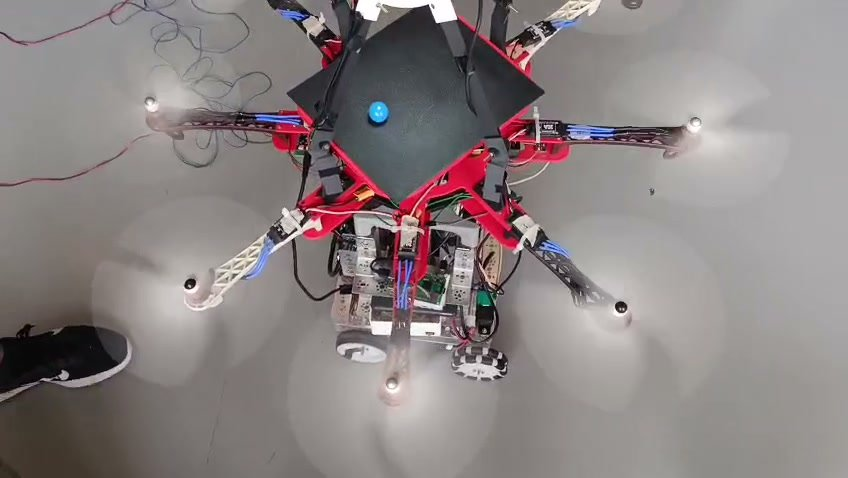
\includegraphics[width=\linewidth]{figures/photo_flat_turn.jpg}\caption{Flat-ground turn.}\end{subfigure}\hfill
  \begin{subfigure}[b]{0.32\textwidth}\centering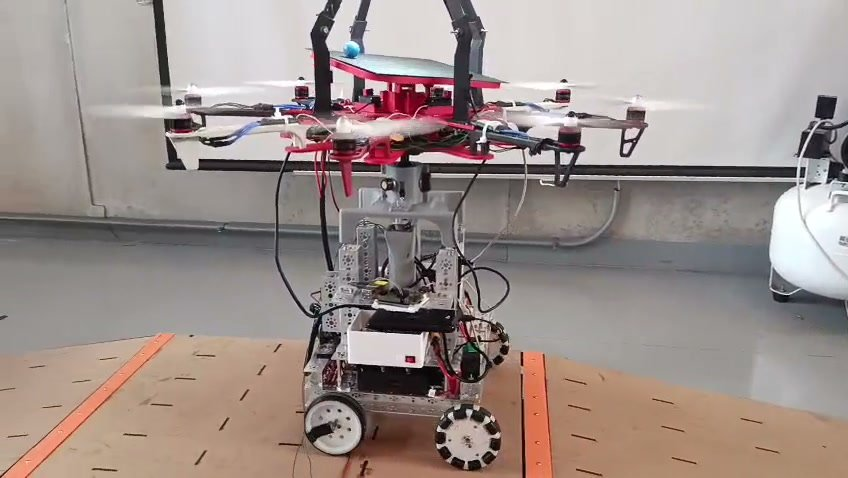
\includegraphics[width=\linewidth]{figures/photo_ramp_climb.jpg}\caption{Climbing the ramp.}\end{subfigure}\hfill
  \begin{subfigure}[b]{0.32\textwidth}\centering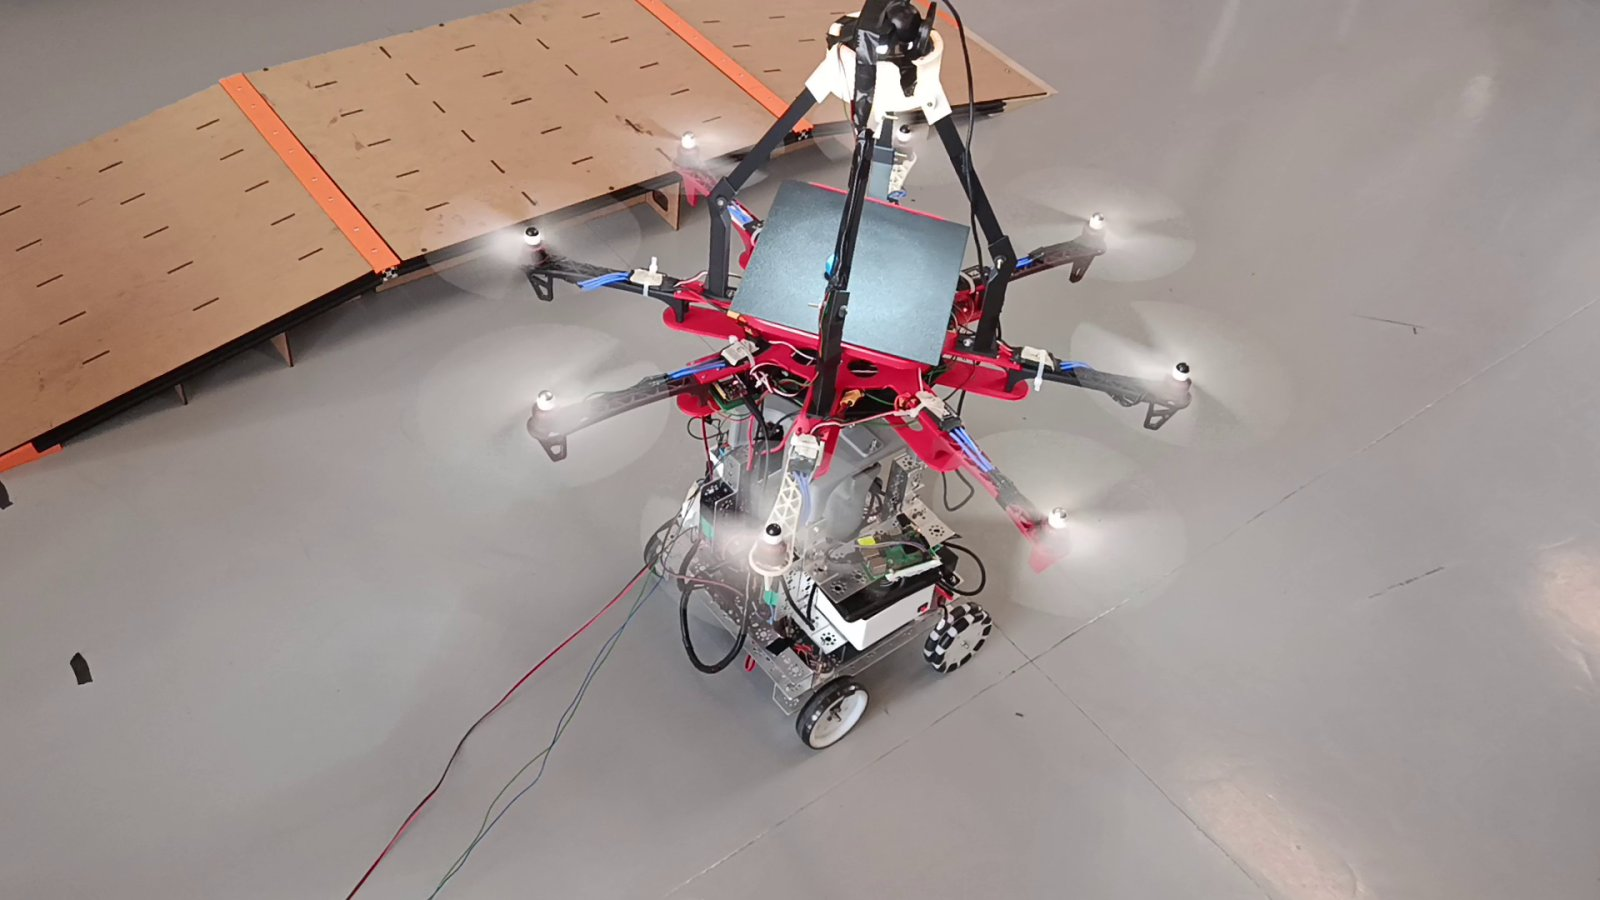
\includegraphics[width=\linewidth,trim=200 0 200 0,clip]{figures/photo_ramp_top.jpg}\caption{At the top of the ramp.}\end{subfigure}
  \caption{Integrated tests on November 18, 2026, with rotors spinning and the ball on the plate (frames from test videos).}
  \label{fig:tests}
\end{figure}

\subsection{Final full-robot trials (Nov.~23)}
\label{sec:ensayos23}
On Nov.~23, ball balancing was repeated on the full robot---the TETRIX mobile base carrying the octocopter on the spherical joint with the ball-and-plate assembly on top---running drone firmware v11 (Sections~\ref{sec:altura} and \ref{sec:metodologia}). We recorded \textbf{13 balancing trials} lasting 23--\SI{122}{\second}, totaling \SI{816}{\second}; in 10 of them, all eight rotors were spinning (\SI{614}{\second}). A trial begins when the PID detects the ball on the plate and ends when the ball leaves the plate or the operator stops it; the first \SI{3}{\second}, during which the ball is placed by hand, are discarded. Table~\ref{tab:ensayos23} and Fig.~\ref{fig:ensayos23} summarize these trials.

\paragraph{Data sources and verification} The Raspberry Pi logged ball position at \SI{187}{\hertz} (\texttt{registro\_20261123\_182316.csv}, 18:23--18:39), but its logs before and after that window could not be downloaded prior to reporting. For those trials, telemetry was recovered from two screen recordings of the web interface (17:29 and 18:36): the page renders the live ball position on the plate map and drone tilt over its 2, 5, and \SI{12}{\degree} rings, and \texttt{extraer\_de\_grabacion.py} measures those markers frame by frame (about \SI{13}{\hertz}) using the page's exact drawing scales. On intervals covered by both the recording and the Pi log, recovered positions differ from logged values by a median of 0.6 and \SI{1.4}{\milli\metre} (P90 of \SI{6.4}{\milli\metre}; 4007 samples), well below the reported errors, so both sources are analyzed together. Screen recovery does not yield servo pulses or drone collective, but it captures plate and motor states.

\begin{table}[!htbp]
\centering
\caption{Ball-balancing trials on the full robot (November 23, 2026). Rot.: rotors spinning. Source: Raspberry Pi log at \SI{187}{\hertz} or telemetry recovered from screen recording. Errors in mm; relative error $e_{\mathrm{RMS}}/R_u$ in \%; effectiveness: \% of time with $e\le\SI{50}{\milli\metre}$. $^\ast$: full-system trial with the base crossing the ramp (Table~\ref{tab:completos23}).}
\label{tab:ensayos23}
\footnotesize
\setlength{\tabcolsep}{3.5pt}
\begin{tabular}{@{}clrclrrrrrc@{}}
\toprule
Trial & Time & $t$ (s) & Rot. & Source & Median & RMS & P95 & Rel.\ err. & Effect. & $\sigma_x$ / $\sigma_y$ \\
 & & & & & & & & & ($\le$\SI{50}{\milli\metre}) & \\
\midrule
01 & 17:30 & 27.0 & yes & video & 29.2 & 33.7 & 56.2 & 34.9 & 88.5 & 30.9 / 11.1 \\
02 & 17:32 & 98.5 & yes & video & 31.8 & 35.3 & 54.9 & 36.6 & 90.5 & 32.3 / 14.3 \\
03 & 17:45 & 122.3 & no & video & 31.5 & 35.0 & 55.7 & 36.3 & 92.1 & 31.2 / 15.7 \\
04 & 18:25 & 22.9 & no & Pi & 44.0 & 51.9 & 94.0 & 53.8 & 63.3 & 49.3 / 11.8 \\
05 & 18:26 & 95.9 & yes & Pi & 39.2 & 51.0 & 99.2 & 52.9 & 67.9 & 49.2 / 13.4 \\
06 & 18:33 & 57.0 & no & Pi & 31.3 & 45.1 & 97.1 & 46.7 & 77.5 & 41.6 / 14.9 \\
07 & 18:36 & 83.5 & yes & Pi & 33.5 & 38.3 & 63.9 & 39.7 & 81.2 & 35.5 / 14.4 \\
08 & 18:40 & 57.4 & yes & video & 42.8 & 46.1 & 72.8 & 47.7 & 65.4 & 40.8 / 20.9 \\
09 & 18:45 & 60.6 & yes & video & 35.1 & 47.3 & 86.5 & 49.0 & 70.2 & 43.4 / 18.8 \\
10$^\ast$ & 18:49 & 39.1 & yes & video & 33.2 & 41.4 & 67.8 & 42.9 & 71.7 & 38.4 / 12.7 \\
11$^\ast$ & 18:51 & 54.7 & yes & video & 42.0 & 48.0 & 82.9 & 49.7 & 67.1 & 38.3 / 28.1 \\
12$^\ast$ & 18:55 & 45.3 & yes & video & 33.4 & 42.6 & 77.4 & 44.1 & 75.7 & 37.2 / 19.6 \\
13$^\ast$ & 19:00 & 51.5 & yes & video & 33.5 & 41.0 & 73.2 & 42.5 & 77.3 & 38.4 / 14.4 \\
\midrule
\multicolumn{5}{@{}l}{Median across 13 trials} & 33.5 & 42.6 & 73.2 & 44.1 & 75.7 & 38.3 / 14.4 \\
\bottomrule
\end{tabular}
\end{table}

\begin{figure}[!htbp]
  \centering
  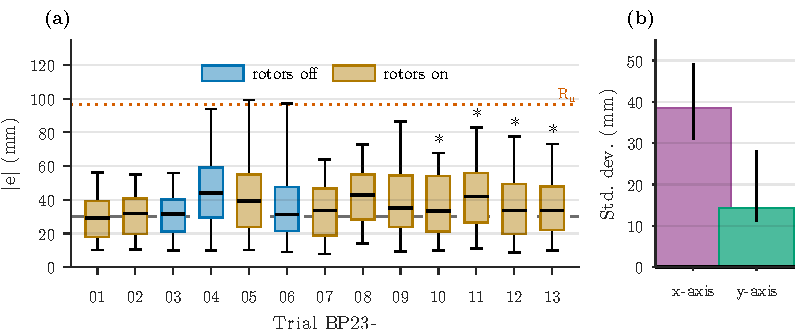
\includegraphics[width=\textwidth]{figures/fig_ensayos_23nov.pdf}
  \caption{Nov.~23 trials on the full robot. (a) Ball error distribution in each trial; the dashed line marks \SI{30}{\milli\metre} and the dotted line marks the usable plate radius. (b) Position standard deviation along each axis (bar: median of the 13 trials; whiskers: minimum and maximum).}
  \label{fig:ensayos23}
\end{figure}

\paragraph{Results}
\begin{itemize}
  \item \textbf{Thirteen continuous balancing segments of 23--\SI{122}{\second} were recorded}, with a median error of 29--\SI{44}{\milli\metre} and 63--92\% of the time within \SI{50}{\milli\metre} of center. The three trials from 17:30--17:47 (BP23-01 to 03) performed best: 29--\SI{32}{\milli\metre} median and 89--92\% of the time within \SI{50}{\milli\metre}, with rotors spinning in two of them. Relative error meets the $\le\SI{45}{\percent}$ criterion of Table~\ref{tab:metricas} in 7 of 13 trials and falls between 46 and \SI{54}{\percent} in the rest; effectiveness in the \SI{30}{\milli\metre} band (25--52\%) does not meet the \SI{60}{\percent} criterion.
  \item \textbf{The rotors do not degrade balancing.} With rotors spinning, drone tilt was 0.71--\SI{1.0}{\degree} RMS, and trials with and without rotors share the same median error (Fig.~\ref{fig:ensayos23}a). The drone kept the plate level across all 10 trials with zero cutoffs.
  \item \textbf{The $x$-axis dominates the error.} Spread along $x$ (31--\SI{49}{\milli\metre}) is 2.7 times that along $y$ (11--\SI{28}{\milli\metre}) in every trial. Along $x$, the ball oscillates side to side with a period of roughly \SI{10}{\second} (Fig.~\ref{fig:bp23despegue}), and the $x$ servo operates with a mean bias of $+65$ to $+\SI{80}{\micro\second}$ above its neutral (\SI{1386}{\micro\second}), reaching its \SI{1612}{\micro\second} stop, whereas the $y$ servo operates centered. This indicates an $x$-axis leveling offset on the plate mounted atop the drone: it consumes one-third of servo travel on that side, and the oscillation is the limit cycle caused by saturation interacting with the integrator. The drone is not the cause, because the same offset appears with the rotors off. Re-leveling the $x$ neutral on the assembled robot (via the Pi's \texttt{/nivelar} routine) directly fixes this.
  \item \textbf{Comparison with Nov.~17--18.} With the base stationary and rotors at idle, the Nov.~17 median was \SI{18.9}{\milli\metre}, compared to 29--\SI{44}{\milli\metre} on Nov.~23. Because the Nov.~23 median $y$-axis spread is \SI{14}{\milli\metre} and the excess error lies in $x$, the difference is attributed to that axis offset, which was absent in earlier sessions.
  \item \textbf{Servo power failure (18:31--18:33).} During this interval, pulse commands varied between 1200 and \SI{1580}{\micro\second}, yet the ball moved less than \SI{0.1}{\milli\metre}: the servo power supply was disconnected. A direct servo check identified the fault, and this interval is excluded from the trials.
\end{itemize}

\paragraph{Full-system trials: base crossing the ramp with drone and ball} In four trials (BP23-10 to 13), the mobile base drove across the \SI{10}{\degree} ramp while the drone---with all eight rotors spinning---leveled the plate and the PID balanced the ball. Motion is confirmed independently in two ways: the LabVIEW screen recording (18:48--19:10, Fig.~\ref{fig:completos23}d) displays the \texttt{ADELANTE} command at 25\% PWM (23\% on the right wheel due to the 0.92 trim) during those intervals, and handheld videos \texttt{VID\_20261123\_184731}, \texttt{\_185130}, \texttt{\_185429}, \texttt{\_190032}, and \texttt{\_190131} (whose filenames encode their start times) show the robot climbing and crossing the ramp transitions (Fig.~\ref{fig:completos23}a--c). Table~\ref{tab:completos23} isolates the moving-base segments.

\begin{table}[!htbp]
\centering
\caption{Nov.~23 full-system trials: base crossing the \SI{10}{\degree} ramp, drone with rotors spinning, and ball balancing. Ball metrics computed only while LabVIEW issued the \texttt{ADELANTE} command.}
\label{tab:completos23}
\small
\begin{tabular}{@{}lrrrrrr@{}}
\toprule
Trial & Moving & Median & P95 & Effect. & Drone RMS & Drone max. \\
 & base (s) & (mm) & (mm) & ($\le$\SI{50}{\milli\metre}) & tilt (\si{\degree}) & tilt (\si{\degree}) \\
\midrule
BP23-10 & 22.9 & 29.6 & 53.7 & 91\,\% & 1.15 & 6.7 \\
BP23-11 & 29.5 & 34.5 & 74.6 & 81\,\% & 0.85 & 4.4 \\
BP23-12 & 18.2 & 30.7 & 52.9 & 89\,\% & 0.99 & 2.3 \\
BP23-13 & 19.0 & 30.6 & 74.7 & 80\,\% & 0.94 & 2.3 \\
\bottomrule
\end{tabular}
\end{table}

\begin{figure}[!htbp]
  \centering
  \begin{subfigure}[b]{0.32\textwidth}\centering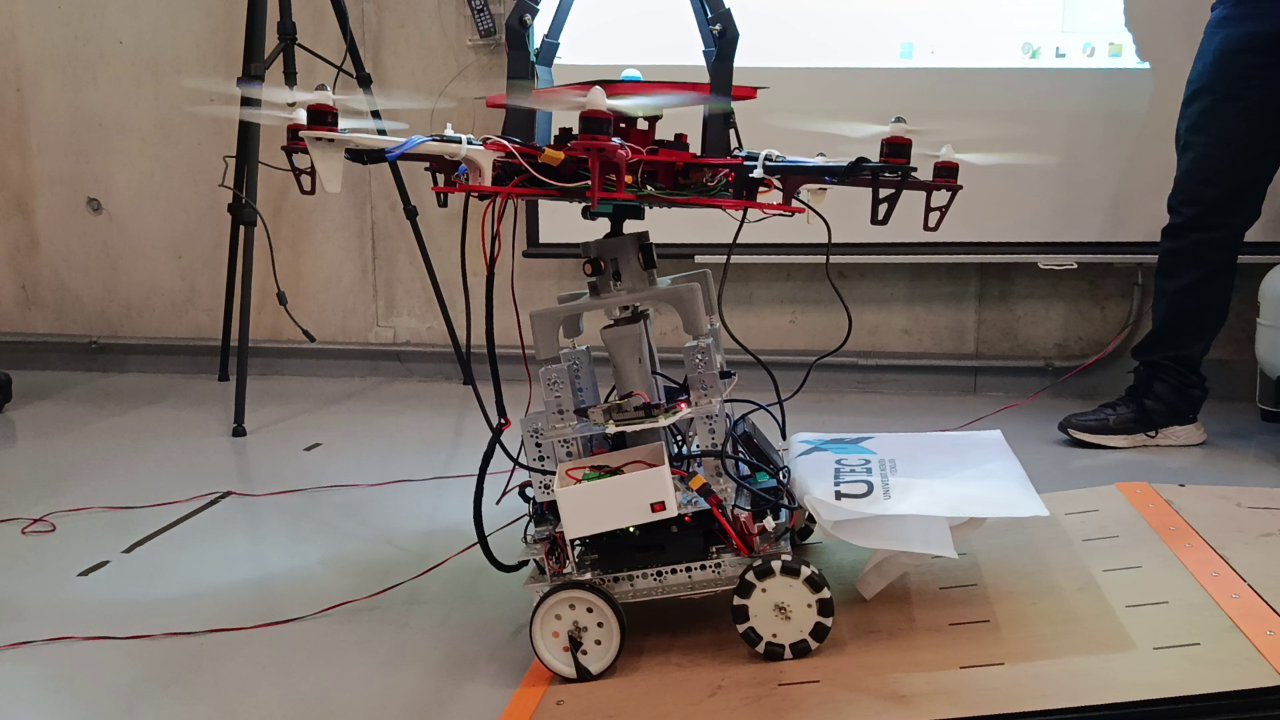
\includegraphics[width=\linewidth]{figures/ensayo23_a.jpg}\caption{BP23-12, 18:55:44.}\end{subfigure}\hfill
  \begin{subfigure}[b]{0.32\textwidth}\centering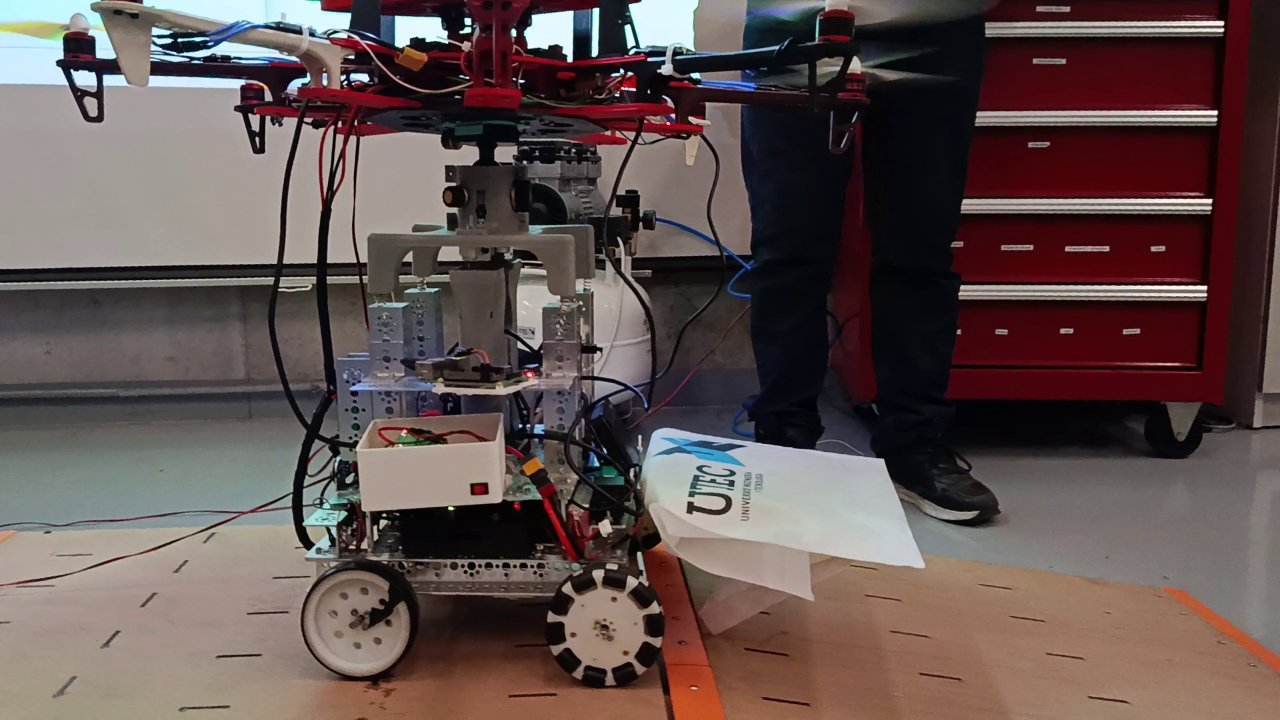
\includegraphics[width=\linewidth]{figures/ensayo23_b.jpg}\caption{BP23-12, 18:55:56.}\end{subfigure}\hfill
  \begin{subfigure}[b]{0.32\textwidth}\centering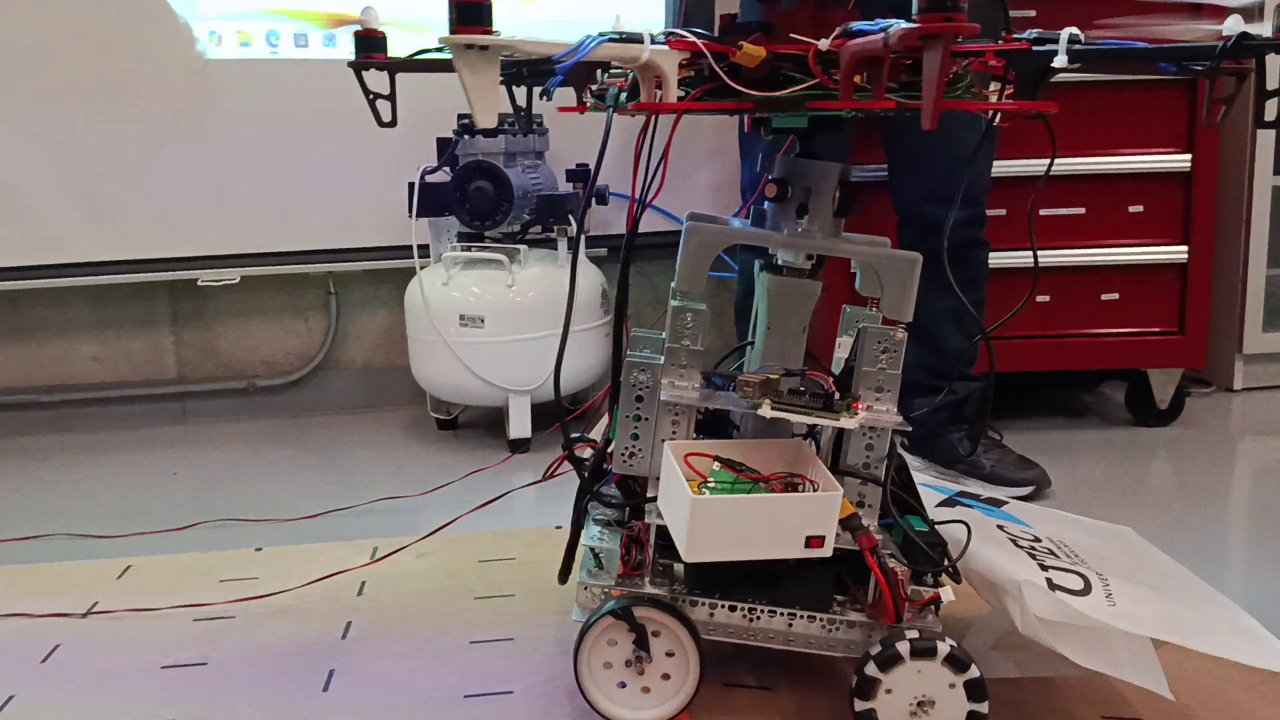
\includegraphics[width=\linewidth]{figures/ensayo23_c.jpg}\caption{BP23-13, 19:01:34.}\end{subfigure}\\[4pt]
  \begin{subfigure}[b]{0.7\textwidth}\centering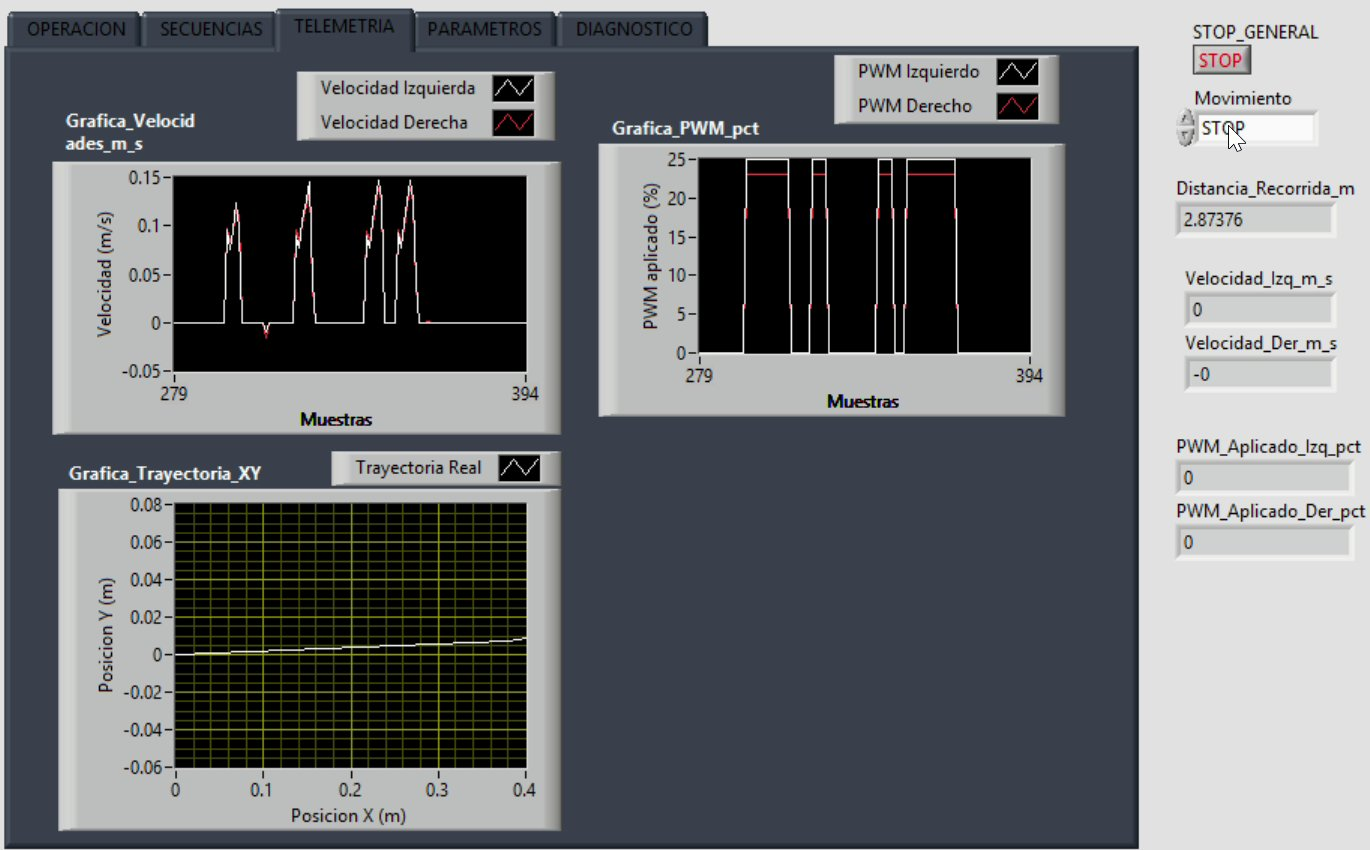
\includegraphics[width=\linewidth]{figures/ensayo23_labview.jpg}\caption{LabVIEW telemetry, 18:49:28.}\end{subfigure}
  \caption{Nov.~23 full-system trials. (a)--(c) The robot crosses the ramp with all eight rotors spinning and the ball on the plate (videos \texttt{VID\_20261123\_185429} and \texttt{\_190131}). (d) myRIO telemetry panel during trial BP23-10: wheel speeds, applied PWM (25/23\,\%), odometry trajectory, and \texttt{ADELANTE} command.}
  \label{fig:completos23}
\end{figure}

During the crossing, the ball stayed within a median of 30--\SI{35}{\milli\metre} from center and 80--91\% of the time within \SI{50}{\milli\metre}---an error equal to or smaller than with the base stationary in the same trials (35--\SI{56}{\milli\metre}) and comparable to the Nov.~18 ramp runs (\SI{29.5}{\milli\metre} median, Table~\ref{tab:bp}). Drone tilt was 0.85--\SI{1.15}{\degree} RMS, with peaks up to \SI{6.7}{\degree} at the transitions, and firmware v11 triggered zero motor cutoffs---unlike the Nov.~18 runs, which ended due to yaw and tilt cutoffs in the bench firmware (Section~\ref{sec:integrated}). The ball stayed on the plate for 18--\SI{30}{\second} of crossing in each trial, on the order of a full traversal of the measured ramp (\SI{2.2}{\metre}; the model predicts \SI{19}{\second} at 25\% PWM, Table~\ref{tab:modelval}). All four trials ended during the crossing as the ball rolled off the plate in the final segment (in BP23-13, while descending the last transition, Fig.~\ref{fig:completos23}c), the same region where drops concentrated on Nov.~18.

\paragraph{Base: speed and straightness} LabVIEW telemetry logged wheel speeds during the Nov.~23 runs. At 25\% PWM, it read 0.078--\SI{0.084}{\metre\per\second} on some segments and 0.124--\SI{0.134}{\metre\per\second} on others. Equation~\eqref{eq:vss} with the measured \SI{10.4}{\kilo\gram} mass predicts \SI{0.078}{\metre\per\second} climbing \SI{10}{\degree} and \SI{0.124}{\metre\per\second} on flat ground, so both groups match the two predictions within 8\%; because telemetry does not flag the current ramp segment, each group is assigned to a segment by proximity. At 40\% PWM, readings ranged from 0.110 to \SI{0.222}{\metre\per\second}, with the peak sitting 8--10\% above the \SI{0.201}{\metre\per\second} flat-ground model prediction. Over a \SI{2.16}{\metre} straight run, odometry ended with \SI{7.8}{\milli\metre} lateral drift (0.4\%) and \SI{-2.7}{\degree} heading error, using the 0.92 right-wheel trim with the wheel PI controller disabled.

\paragraph{Drone takeoff with the ball aboard} In trial BP23-05, hovering was commanded while the ball was balancing (Fig.~\ref{fig:bp23despegue}). The collective ramped from 1300 to \SI{1750}{\micro\second} over \SI{25}{\second} without losing the ball. At 18:28:04, the module lifted off along the vertical guide: the laser reading rose from 385 to \SI{499}{\milli\metre} (a \SI{114}{\milli\metre} climb) with tilt staying within \SI{2.5}{\degree}, and landed cleanly on the land command with zero cutoffs. This was the tenth flight on the guide (the first with firmware v11) and the first carrying the plate and ball. However, the ball---which sat at center ($x=\SI{-1}{\milli\metre}$) half a second earlier---left the plate within \SI{0.5}{\second}: the module jumps upward rather than rising smoothly because guide friction holds it until thrust breaks stiction, and the accelerometer recorded 0.28 to \SI{1.5}{g} at that instant. The plate cannot compensate vertical acceleration, so the fix lies in the takeoff sequence: ramp more slowly near liftoff thrust and engage the cascaded altitude controller (Section~\ref{sec:altura}) as soon as the laser detects upward motion, preventing continued upward acceleration.

\begin{figure}[!htbp]
  \centering
  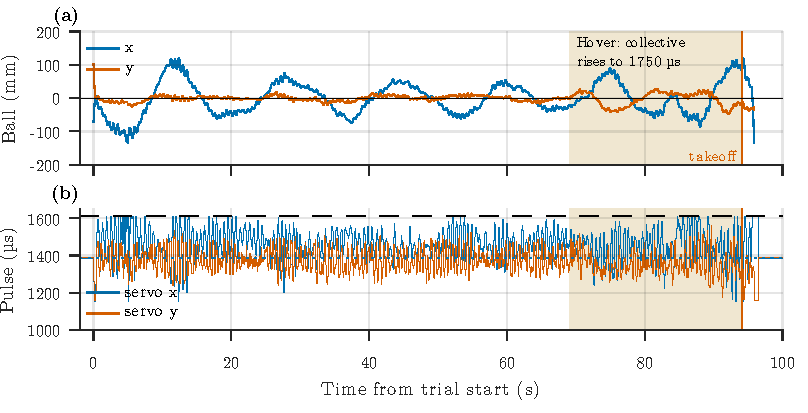
\includegraphics[width=\textwidth]{figures/fig_bp23_despegue.pdf}
  \caption{Trial BP23-05 (Raspberry Pi log at \SI{187}{\hertz}). Top: ball position; bottom: servo pulses, with the $x$-axis neutral (dotted) and upper stop (dashed). The shaded band marks the collective ramp up to \SI{1750}{\micro\second}, and the red line marks drone takeoff, when the ball leaves the plate. Both the slow $x$-axis oscillation and the $x$-servo bias above neutral are visible.}
  \label{fig:bp23despegue}
\end{figure}

\subsection{Mobile base and integrated tests}
\label{sec:integrated}
Fig.~\ref{fig:tests} shows frames from the integrated tests. Carrying the drone with rotors spinning and the ball on the plate, the mobile base completed:
\begin{itemize}
  \item straight runs and turns on flat ground;
  \item climbs and descents of the \SI{10}{\degree} ramp in both directions, repeated over multiple passes (test videos in the repository's \texttt{videos/} folder).
\end{itemize}
In the eight integrated runs of Nov.~18, the drone ran the bench firmware at a \SI{1300}{\micro\second} collective---providing no weight relief ($f\approx0$)---and the runs ended as follows:
\begin{itemize}
  \item four due to the \SI{20}{\degree} yaw cutoff, as the drone rotated with the base;
  \item three due to the \SI{12}{\degree} tilt cutoff, measured at 12.0--\SI{12.2}{\degree} with angular rates up to \SI{49}{\degree\per\second} upon entering the ramp, leaving only \SI{2}{\degree} of margin on a \SI{10}{\degree} slope;
  \item one stopped by the operator.
\end{itemize}
These events confirm the coupling predicted by \eqref{eq:pitchlin}: spherical-joint acceleration at the ramp edges acts on the module through the $-mh_ca_J$ term, and the slow attitude mode amplifies it (Fig.~\ref{fig:transm}b). The UART link between the myRIO and the Pi was implemented on both ends and verified on the Pi using a simulated serial port: valid frames executed, invalid frames were rejected, myRIO priority was respected, and 6-field telemetry was generated. It was then tested with the myRIO connected (Fig.~\ref{fig:uart}): the Pi transmitted ball position over UART, and the myRIO VI received and plotted it in real time on its $x$--$y$ graph, spanning the full plate ($\pm$\SI{150}{\milli\metre}) as the ball moved; the received-character indicator stayed lit throughout the test. In that test, the drone roll and pitch plots remained blank, so drone-to-myRIO telemetry remains to be verified, and the session ended with LabVIEW reporting a lost connection to the myRIO.

\begin{figure}[!htbp]
  \centering
  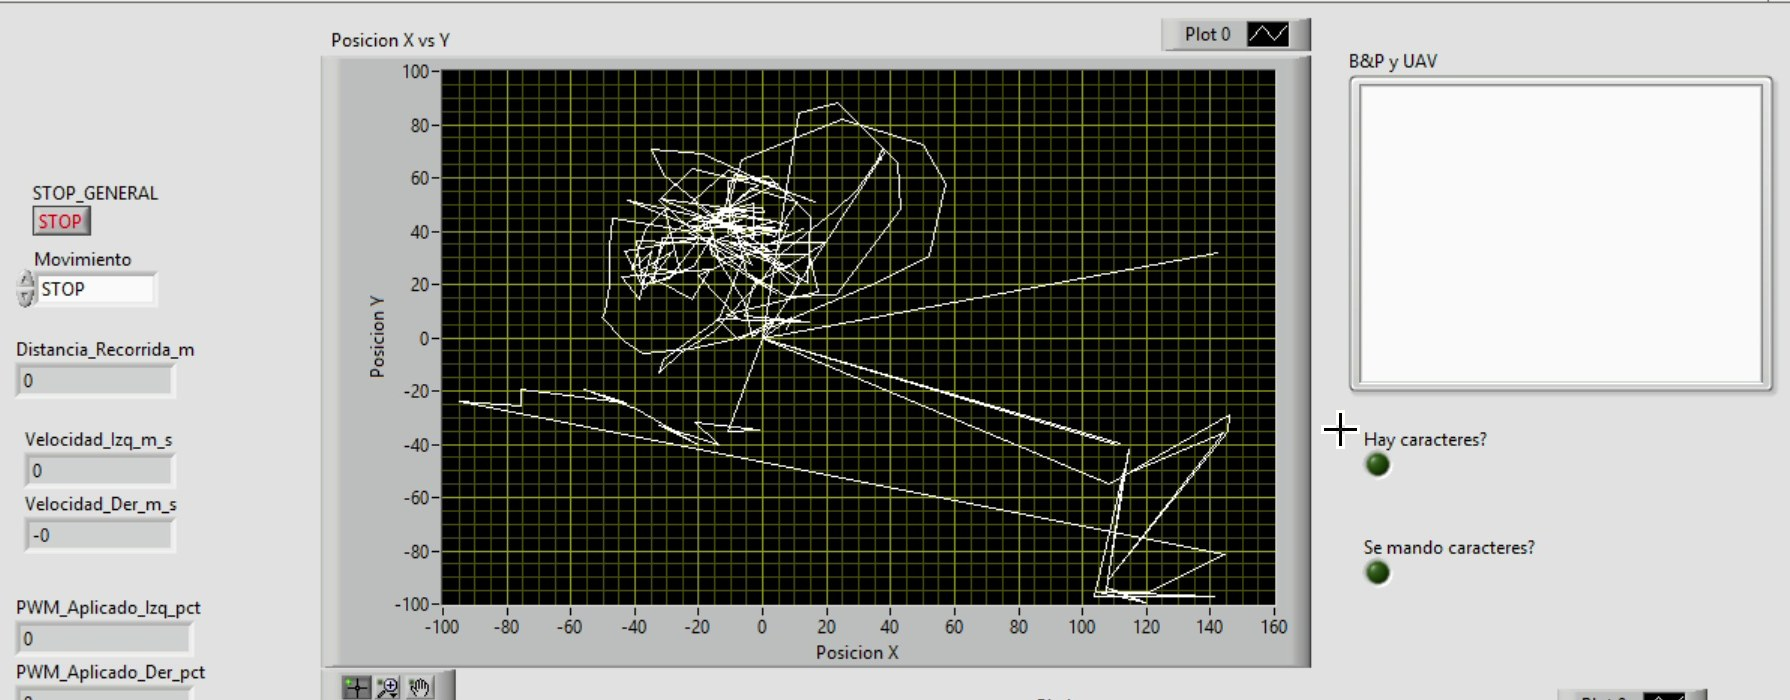
\includegraphics[width=0.9\textwidth]{figures/uart_myrio_bola.jpg}
  \caption{UART link test between the Raspberry Pi and the myRIO: LabVIEW panel showing ball position received from the Pi ($x$--$y$ graph, in mm), the received string (\texttt{B\&P y UAV}), and transmit/receive indicators.}
  \label{fig:uart}
\end{figure}

%% ---- TODO after final base trials: populate and uncomment this table ----
% \begin{table}[!htbp]\centering\small
% \caption{Final base trials (odometry and video). Error = |final position - target|.}
% \begin{tabular}{@{}lrrrr@{}}\toprule
% Trial & Target & Measured (mean $\pm$ SD, $n$) & Error (\%) & Median ball error (mm) \\\midrule
% Translation, flat & 25 cm & & & \\
% Translation, flat & 50 cm & & & \\
% Translation, 10 degrees & 25 cm & & & \\
% Turn about axle midpoint & 360 degrees & & & \\
% Turn about one wheel & 360 degrees & & & \\
% 10-degree climb in ramp mode (f = 0.5) & -- & & & \\
% \bottomrule\end{tabular}\end{table}

\subsection{Model validation}
\label{sec:modelval}
Table~\ref{tab:modelval} compares the predictions of the Section~\ref{sec:model} model against measurements. Parameters identified from a dataset are marked; comparisons in all other rows use data not used to construct the model.

\begin{small}
\setlength{\tabcolsep}{4pt}
\begin{longtable}{@{}>{\raggedright\arraybackslash}p{0.25\textwidth}>{\raggedright\arraybackslash}p{0.22\textwidth}>{\raggedright\arraybackslash}p{0.34\textwidth}>{\raggedright\arraybackslash}p{0.11\textwidth}@{}}
\caption{Model predictions versus measurements.}\label{tab:modelval}\\
\toprule
Quantity & Model & Measurement & Eq./Sec. \\
\midrule\endfirsthead
\toprule Quantity & Model & Measurement & Eq./Sec. \\ \midrule\endhead
Base speed, 15\%, flat & \SI{0.072}{\metre\per\second} & 0.06--\SI{0.08}{\metre\per\second} (LabVIEW telemetry) & \eqref{eq:vss} \\
Base speed, 15\%, \SI{10}{\degree} & \SI{0.027}{\metre\per\second} & ramp climbed more slowly than flat ground (videos) & \eqref{eq:vss} \\
Base speed, 25\%, flat / \SI{10}{\degree} (Nov.~23) & 0.124 / \SI{0.078}{\metre\per\second} & 0.124--0.134 / 0.078--\SI{0.084}{\metre\per\second} (LabVIEW), error $\le\SI{8}{\percent}$ & \eqref{eq:vss} \\
Base speed, 40\%, flat (Nov.~23) & \SI{0.201}{\metre\per\second} & peak 0.217--\SI{0.222}{\metre\per\second} (+8 to +10\%) & \eqref{eq:vss} \\
Hover collective & \SI{1899}{\micro\second} (firmware map); \SI{1770}{\micro\second} (audit) & liftoff at \SIrange{1725}{1775}{\micro\second} & \ref{sec:ident} \\
Takeoff with discharged battery (Flight~9) & \SI{1787}{\micro\second} (1758--1817) & \SI{1796}{\micro\second} & \eqref{eq:ureq} \\
Takeoff at 11.1\,V at rest & 1850--\SI{2000}{\micro\second}: cannot sustain hover & did not hover & \eqref{eq:ureq} \\
Module center of mass & $h_c=\SI{0.10}{\metre}$ (CAD) & $h_c=0.14\pm\SI{0.06}{\metre}$, $\delta_x=9.5\pm\SI{1.8}{\milli\metre}$ (identified) & \eqref{eq:cop} \\
Recoverable tilt, v4--v7 limits & $\theta^\ast=$ 2.8--\SI{3.8}{\degree} & Flights~3--6 drifted to the \SI{12}{\degree} interlock & \eqref{eq:thetastar} \\
Recoverable tilt, v8--v9 limits & $\theta^\ast=$ 16--\SI{19}{\degree} & Flights~7--9 held for 20--\SI{48}{\second} & \eqref{eq:thetastar} \\
Slow attitude mode in hover & 0.20--\SI{0.30}{\hertz}, $\zeta=$ 0.24--0.42 & spectral peaks at 0.15--\SI{0.23}{\hertz} & \ref{sec:attitude} \\
Ball loop, derivative gain & stable at 4.5, unstable at 6 for $K_{b,\mathrm{eff}}=$ 3.5--4.9 & 4.5 stable, 6 unstable (bench) & \ref{sec:ballcontrol} \\
Ball plant gain & 6.0 (CAD); 3.5--4.9 (inferred) & 2.5 / 4.9 ($x$/$y$, regression, $R^2\le0.45$) & \eqref{eq:balltf} \\
Ball error from attitude, rotors on & 1.7--\SI{2.1}{\milli\metre} RMS & 16--\SI{21}{\milli\metre} RMS (dominated by $D_b$) & \eqref{eq:propag} \\
Ball error, stationary vs.\ moving base & increase from base accelerations & median +9 to \SI{11}{\milli\metre} & \eqref{eq:balllinx} \\
Static tip-over angle (locked module) & CAD CoM: $x_G=\SI{81}{\milli\metre}$ & \SI{21.5}{\degree} uphill and \SI{30.5}{\degree} downhill (Nov.~23), giving $x_G=\SI{88}{\milli\metre}$: CAD differs by \SI{8}{\percent} & \eqref{eq:tip} \\
Vertical guide travel & \SI{77}{\milli\metre} (CAD) & about \SI{140}{\milli\metre} (measured) & Table~\ref{tab:params} \\
Spherical joint range vs.\ ramp transitions & required $>\SI{10}{\degree}$ & 35--\SI{53}{\degree} depending on direction & Sec.~\ref{sec:metodologia} \\
Altitude via calibrated laser and Kalman filter & \SI{330}{\milli\metre} (ruler) & 317--\SI{334}{\milli\metre} (error $\le\SI{4}{\percent}$) & \eqref{eq:kfz} \\
Cascaded altitude control & 4--\SI{12}{\milli\metre} peak-to-peak (simulation) & not flight-tested; laser with Kalman filter logged Flight~10 takeoff (\SI{114}{\milli\metre} climb) & \eqref{eq:cascada} \\
Ramp cycle (\SI{0.7}{\metre} at \SI{10}{\degree} + \SI{0.8}{\metre} + \SI{0.7}{\metre}), \SI{15}{\percent} PWM & \SI{41}{\second} at idle; \SI{37}{\second} in ramp mode & pending (stopwatch) & \eqref{eq:vss}, \eqref{eq:descarga} \\
Ramp crossing at \SI{25}{\percent} PWM (Nov.~23) & \SI{19}{\second} & \SI{25.5}{\second} \texttt{ADELANTE} command in BP23-12; ball held 18--\SI{30}{\second} during crossing & \eqref{eq:vss}, \eqref{eq:descarga} \\
\bottomrule
\end{longtable}
\end{small}

The model reproduces every measured quantity, mostly within parameter uncertainty. Its main open discrepancy is the magnitude of the direct ball disturbance, $D_b$, which the model treats as an external input; quantifying rotor airflow over the plate is the natural next experiment. Weight-relief predictions on the ramp have not yet been measured.

\subsection{Requirements compliance and limitations}
\label{sec:requirements}
\label{sec:limits}
Table~\ref{tab:req} compares our results against the validation scenarios in the course guide.

\begin{table}[!htbp]
\centering
\caption{Status of the project guide validation scenarios.}
\label{tab:req}
\footnotesize
\renewcommand{\arraystretch}{1.1}
\begin{tabularx}{\textwidth}{@{}>{\raggedright\arraybackslash}p{0.34\textwidth}>{\raggedright\arraybackslash}X>{\raggedright\arraybackslash}p{0.17\textwidth}@{}}
\toprule
Scenario & Evidence & Status \\
\midrule
Base translation and rotation (flat, \SI{10}{\degree}) & ramp climbed and descended in both directions; Nov.~23 speeds within 8--10\% of model; 0.4\% lateral drift over \SI{2.16}{\metre}; odometry modes for \SI{25}{\centi\metre}, \SI{50}{\centi\metre}, and \SI{360}{\degree} implemented & met for translation; rotation lacks final metric \\
Base on \SI{20}{\degree} slope & not tested; without thrust, measured static tip-over angle is \SI{21.5}{\degree} (\SI{0.26}{\metre\per\second\squared} margin at \SI{20}{\degree}); with ramp mode ($f=0.35$--0.55), margin rises to 0.72--\SI{0.98}{\metre\per\second\squared} (Section~\ref{sec:porquedron}) & not met; feasible with ramp mode, unvalidated \\
Platform and ball estimation & detection at \SI{187}{fps} across the full plate; homography calibration & met \\
Balancing with stationary base & median 4.4 / \SI{18.9}{\milli\metre} (drone off / on, Nov.~17), zero drops; 13 continuous segments of 23--\SI{122}{\second} on Nov.~23 (\SI{816}{\second}, 10 with rotors), median 29--\SI{44}{\milli\metre} (Table~\ref{tab:ensayos23}) & met \\
Balancing during translation (flat, \SI{10}{\degree}) & median 27.9 / \SI{29.5}{\milli\metre} (Nov.~18), P95 below plate half-width; four Nov.~23 full-system ramp crossings with rotors spinning: median 30--\SI{35}{\milli\metre}, 18--\SI{30}{\second} crossing, zero drone cutoffs (Table~\ref{tab:completos23}) & met, with drops on the final ramp segment \\
Balancing during rotation & runs with turns included in condition~(c) & partially met (yaw cutoffs) \\
Intermediate stage (octocopter) & bench RMS $<$\SI{0.4}{\degree}; three hovers on the vertical guide of \SIrange{20}{48}{\second} (Flights~7--9); 0.71--\SI{1.0}{\degree} RMS with rotors and tray aboard (Nov.~23); cutoff-free takeoff and landing with ball aboard (Flight~10, v11) & met on the guide \\
Interface and logging & web interface, LabVIEW panel, CSV logs at camera and drone rates & met \\
\bottomrule
\end{tabularx}
\end{table}

The main limitations are:
\begin{enumerate}[label=(\roman*)]
  \item \textbf{Cutoffs during integrated runs and pending v11 features.} During the Nov.~18 runs, the bench firmware cut off on yaw (\SI{20}{\degree}) and tilt (\SI{12}{\degree}). Firmware v11 resolved the idle yaw cutoff ($\le\SI{1400}{\micro\second}$) via a $\pm\SI{20}{\degree}$ sliding window with a \SI{120}{\degree\per\second} safety ceiling, enabling all four Nov.~23 ramp crossings without cutoffs. Scaling the \SI{12}{\degree} tilt limit with slope and validating active yaw tracking (\texttt{yb}) from the myRIO over full \SI{360}{\degree} turns remain pending.
  \item \textbf{Unmonitored battery voltage.} The firmware does not measure LiPo voltage, yet thrust margin drops with voltage squared: useful sustained flight lasts 3--\SI{7}{\minute} per battery pair, and at 11.1\,V at rest the module no longer lifts off below the sustained limit (Section~\ref{sec:bateria}).
  \item \textbf{Pending protocol tests (future work).} The Nov.~23 campaign did not execute ramp weight relief ($f=0.5$; runs stayed at idle), comparative test~D (locked drone C2 vs.\ free drone C3), tape-measured repetitions of \SI{25}{\centi\metre}, \SI{50}{\centi\metre}, and \SI{360}{\degree} turns (E1), the sinusoidal plate sweep (E2), or the 2 and \SI{5}{\centi\metre} recovery tests (E3).
  \item \textbf{Center of mass and authority margin.} The \SI{9.5}{\milli\metre} eccentricity demands a permanent \SI{0.31}{\newton\metre} trim torque, and the center-of-mass height above the spherical joint ($h_c\approx\SI{0.14}{\metre}$) leaves a small net attitude-loop stiffness (Section~\ref{sec:attitude}).
  \item \textbf{Thrust map.} The thrust map was not identified on a load cell; takeoff data show that $k_F$ is 33--52\% higher than assumed, and its shape at high collective remains unknown.
  \item \textbf{Power system.} The original BMS for the servos and relay coils failed, so a bench power supply was used in part of the tests; GPIO5 and GPIO14 emit startup pulses when the ESP32 boots, requiring the ESCs to be powered only after boot.
  \item \textbf{Vision.} Ball detection relies on color thresholding, so ambient lighting must be controlled.
  \item \textbf{Spherical joint height.} The module center of mass lies above the spherical joint, making the module an inverted pendulum ($h_c=0.14\pm\SI{0.06}{\metre}$, unstable pole at \SI{6.1}{\radian\per\second}) and forcing attitude control near the delay limit $p\theta_e\approx0.5$. Lowering the center of mass below the spherical joint would make it passively stable.
  \item \textbf{Model parameters.} Inertia $\vect J$, base mass distribution, and LiPo internal resistance are estimates derived from CAD, tests, or typical values, and servo lag was inferred rather than measured. A load-cell thrust stand, a bifilar pendulum test for inertia, a servo step-response test, and a loaded voltage-sag measurement would close these gaps.
\end{enumerate}
          % 8. Validation and characterization
%% ======================================================================
%% 10_conclusions.tex -- 9. Conclusions
%% ======================================================================
\section{Conclusions}
\label{sec:conclusions}
AeroTray demonstrates that three independent balancing loops can be stacked on a mobile base using low-cost hardware, and that base-disturbance propagation across them can be both measured with synchronized logs and predicted from a first-principles model. Symbolically verified and parameterized from the CAD assembly, datasheets, and logs, the model yields six experimentally confirmed findings.

(i)~The aerial module behaves as an inverted pendulum on an accelerating pivot whose center of mass, identified from hover telemetry, lies $0.14\pm\SI{0.06}{\metre}$ above the spherical joint and \SI{9.5}{\milli\metre} toward M8. (ii)~The attitude loop works only because proportional stiffness exceeds gravitational stiffness by a narrow margin supplied by the underestimated thrust gain; that narrow margin explains the slow attitude mode observed in hover. (iii)~The slow divergences in early flights were a torque-authority limit, with a region of attraction of only 3--4$^\circ$, and were resolved by widening the angular-rate command limit rather than retuning gains. (iv)~The ball loop is bounded by its delay and by a right-half-plane zero caused by ball height above the plate pivot, which together set the derivative-gain ceiling; effective plant gain is roughly 70\% of the CAD value due to mechanism backlash. (v)~The passive spherical joint removes slope from the ball dynamics, turns are benign, and residual ball error with spinning rotors is dominated by a slowly varying direct aerodynamic and vibrational load rather than octocopter attitude motion.

(vi)~The drone is justified on the ramp for two quantified reasons. By leveling itself, it decouples the slope from the plate and preserves 84--95\% of servo travel, whereas a base-fixed tray would exhaust its travel on an \SI{11}{\degree} slope. By supporting part of its own weight, it acts as adjustable ballast that lowers the effective center of mass: with the rotors carrying half the module weight, the uphill tip-over angle rises from \SI{21.5}{\degree} (measured on the \SI{10.4}{\kilo\gram} full robot) to a predicted \SI{27.7}{\degree}, the downhill tip-over angle rises from \SI{30.5}{\degree} to a predicted \SI{38.2}{\degree}, and the acceleration margin at \SI{20}{\degree} increases by a factor of 3.5. On the ramp, the drone should not hover; instead, it should operate in a 35--55\% weight-relief window at a cost of 2--5\% battery capacity per minute. Conversely, hover thrust margin depends on LiPo voltage squared: at 12.4\,V the module lifts off at 1725--\SI{1775}{\micro\second}, whereas at 11.1\,V it would require 1850--\SI{2000}{\micro\second}, explaining why hover failed at low charge and limiting useful flight to 3--\SI{7}{\minute} per battery pair.

Experimentally, the final firmware holds the \SI{3.6}{\kilo\gram} module on the vertical guide within 0.55--\SI{1.7}{\degree} RMS attitude error, and the ball controller keeps the ball within a median of 19--\SI{30}{\milli\metre} of center on a stationary base, on flat ground, and on a \SI{10}{\degree} ramp. In the final full-robot trials (Nov.~23), 13 balancing trials lasted 23--\SI{122}{\second} (\SI{816}{\second} total; 29--\SI{44}{\milli\metre} median), 10 of them with spinning rotors and the drone leveled at 0.71--\SI{1.0}{\degree} RMS. In four full-system trials, the base crossed the \SI{10}{\degree} ramp with rotors spinning and the ball balancing for 18--\SI{30}{\second} (30--\SI{35}{\milli\metre} median, drone at 0.85--\SI{1.15}{\degree} RMS with zero cutoffs, the ball exiting the plate in the final segment). The module also took off and landed on the vertical guide carrying the tray, though the ball rolled off at liftoff. Base speed measured that day agrees with the model within 8--10\%. Two concrete fixes follow directly from these trials: re-leveling the plate's $x$-axis neutral, which concentrates the error, and smoothing guide takeoff, whose stiction jump dislodged the ball at liftoff. The model also identifies the highest-impact next steps: measuring battery voltage to compensate collective, testing ramp mode, lowering the module center of mass below the spherical joint, shortening ball-loop delay, shielding the plate from rotor airflow, and smoothing base velocity references. All design files, source code, analysis scripts, videos, and raw data are published so these experiments can be reproduced and extended---for example, using the already implemented tilt feedforward or controllers trained on the published model.
         % 9. Conclusions
%% ======================================================================
%% 11_declarations.tex -- ethics, CRediT, competing interest, funding, AI disclosure, acknowledgments, biographies
%% ======================================================================
\section*{Ethics statements}
This work did not involve human subjects, animal experiments, or data collected from social media platforms.

\section*{CRediT author statement}
\textbf{Sebastián Rejas Córdova:} Conceptualization, Methodology, Investigation (integration and verification), Validation, Writing -- review \& editing.
\textbf{George Henry Ramos Astuhuamán:} Software (Raspberry Pi supervisor, vision, octocopter and ESP32-S3 firmware, web interface), Methodology (kinematic and dynamic model, identification), Formal analysis, Data curation, Visualization, Writing -- original draft.
\textbf{Johan Nireo Naupay Fabián:} Methodology, Resources (power system design and audit), Investigation (integration), Writing -- review \& editing.
\textbf{Hideky Edu Garnique Pisfil:} Investigation (flat-ground validation), Software (user interface), Visualization, Writing -- review \& editing.
\textbf{Diego André Miranda Zamora:} Software (LabVIEW base control and myRIO--Pi UART link), Investigation (ramp validation), Writing -- review \& editing.

\section*{Declaration of competing interest}
The authors declare that they have no known competing financial interests or personal relationships that could have appeared to influence the work reported in this paper.

\paragraph{Funding}
\tocheck{This work received no external funding; laboratory equipment from UTEC was used.}

\section*{Declaration of generative AI and AI-assisted technologies in the writing process}
During the preparation of this manuscript, the authors occasionally used the artificial intelligence tools Claude (Anthropic) and Gemini (Google) solely for support in specific tasks:
\begin{itemize}
  \item preliminary literature review and background search;
  \item grammar, spelling, and style editing of the manuscript;
  \item targeted debugging of errors in code written by the team.
\end{itemize}
Mechanical and electrical design, mathematical modeling, prototype construction, subsystem programming, experimental testing, and data analysis were carried out by the authors. After using these tools, the authors reviewed, edited, and verified all technical content, equations, measurements, and software against the source code and experimental logs, and take full responsibility for the content of the publication.

\section*{Acknowledgments}
The authors thank the instructors of the course MT5001 Mechatronic Systems Design (Elvis Jara and Rodrigo Magallanes) and the UTEC laboratory staff for providing equipment (myRIO, TETRIX kit, and bench power supplies) and guidance.

\section*{Biographies}
\noindent\textbf{Sebastián Rejas Córdova} is an undergraduate student in Mechatronics Engineering at UTEC (Lima, Peru). His interests include mechanical design and systems integration for mobile robots.

\noindent\textbf{George Henry Ramos Astuhuamán} is an undergraduate student in Mechatronics Engineering at UTEC. His interests include embedded control, computer vision, and aerial robotics.

\noindent\textbf{Johan Nireo Naupay Fabián} is an undergraduate student in Mechatronics Engineering at UTEC. His interests include power electronics and energy systems for robots.

\noindent\textbf{Hideky Edu Garnique Pisfil} is an undergraduate student in Mechatronics Engineering at UTEC. His interests include human--machine interfaces and experimental validation.

\noindent\textbf{Diego André Miranda Zamora} is an undergraduate student in Mechatronics Engineering at UTEC. His interests include real-time control on NI hardware and inter-robot communication.
        % ethics, CRediT, funding, AI, acknowledgments, biographies

\appendix
%% ======================================================================
%% A_derivations.tex -- Appendix A: derivations and symbolic verification
%% ======================================================================
\section{Derivations and verification}
\label{app:derivations}

\subsection{Ball on an accelerating and rotating plate}
All vectors are expressed in $\{P\}$, which rotates at $\vect\Omega$ and whose origin $G$ has absolute acceleration $\vect a_G$. With $\vect\rho=[x_b,y_b,\varepsilon]\T$ and relative velocity $\dot{\vect\rho}=[\dot x_b,\dot y_b,0]\T$, the absolute acceleration of the ball center is
\begin{equation}
  \vect a_b=\vect a_G+\dot{\vect\Omega}\times\vect\rho+\vect\Omega\times(\vect\Omega\times\vect\rho)+2\,\vect\Omega\times\dot{\vect\rho}+\ddot{\vect\rho}.
  \tag{A.1}
\end{equation}
The ball contact point is $\vect\rho-r_b\ez$. Equating its velocity, $\vect v_G+\vect\Omega\times\vect\rho+\dot{\vect\rho}+\vect\omega_b\times(-r_b\ez)$, to that of the coinciding plate point, $\vect v_G+\vect\Omega\times(\vect\rho-r_b\ez)$, yields the no-slip rolling constraint $\dot{\vect\rho}=r_b\,\vect w\times\ez$ with $\vect w=\vect\omega_b-\vect\Omega$; hence $w_x=-\dot y_b/r_b$, $w_y=\dot x_b/r_b$, and $w_z$ is free. The absolute angular acceleration of the ball is $\dot{\vect\omega}_b=\dot{\vect\Omega}+\dot{\vect w}+\vect\Omega\times\vect w$. With contact force $\vect F=[F_x,F_y,N]\T$, the Newton--Euler equations are
\begin{equation}
  m_b\vect a_b=m_b\vect g_P+\vect F,\qquad I_b\dot{\vect\omega}_b=(-r_b\ez)\times\vect F=[\,r_bF_y,\ -r_bF_x,\ 0\,]\T .
  \tag{A.2}
\end{equation}
The first two components of the rotational equation give $F_x$ and $F_y$; substituting them into the first two components of the translational equation and dividing by $m_b(1+\iota)$ yields \eqref{eq:ballx}--\eqref{eq:bally}, while the third rotational component gives \eqref{eq:spin}. The term $-\kappa\dot\Omega_y$ combines $-\varepsilon\dot\Omega_y$ from the transport acceleration~(A.1) and $-(I_b/m_br_b)\dot\Omega_y$ from the rotational equation: because the ball center lies above the rotation axis, angular acceleration of the plate accelerates the contact surface beneath the ball, producing the right-half-plane zero $z_1$ in \eqref{eq:balltf}. The script \fn{scripts_modelo/derive_ball.py} performs this elimination in SymPy for arbitrary $\vect\Omega(t)$, $\vect a_G(t)$, and $\vect g_P$, confirming that the residual against \eqref{eq:ballx}--\eqref{eq:spin} vanishes identically.

\subsection{Rigid body about an accelerating pivot}
For a rigid body and a point $A$ fixed in it, the angular momentum about $A$ is $\vect H_A=\vect J_A\vect\omega$ (in body-frame components) and, if $A$ accelerates at $\vect a_A$, $\dot{\vect H}_A=\vect M_A-m\,\vect r_{AC}\times\vect a_A$ \cite{ginsberg1998}. Including gravity in $\vect M_A$ and projecting into body axes yields \eqref{eq:euler}. The script \fn{derive_drone.py} constructs $\Rot_{WD}=\Rot_z(\psi)\Rot_y(\theta)\Rot_x(\phi)$, evaluates $m\vect r_c\times\Rot_{WD}\T(\vect g_W-\vect a_J)$, and returns its first-order Taylor expansion,
\begin{equation}
  \begin{bmatrix}m(h_ca_y-\delta_yg+gh_c\phi)\\ m(-h_ca_x+\delta_xg+gh_c\theta)\\ 0\end{bmatrix},
  \tag{A.3}
\end{equation}
which is the gravitational and inertial part of \eqref{eq:rolllin}--\eqref{eq:pitchlin}. The same script inverts the mapping between body angular rates and $z$--$y$--$x$ Euler-angle derivatives, recovering \eqref{eq:euler_rates}, the kinematic law integrated by the firmware.

\subsection{Allocation identities}
For the rotor layout in Table~\ref{tab:params}, with $D=L_r/\sqrt2$, the four diagonal rotors contribute $4D^2=2L_r^2$ and the four axial rotors contribute $2L_r^2$ to both $\sum x_i^2$ and $\sum y_i^2$; all cross sums vanish by symmetry, and $\sum s_i=\sum s_ix_i=\sum s_iy_i=0$ because each spin direction occupies a complete square. Therefore, $\vect B\vect B\T$ in \eqref{eq:alloc} is diagonal and \eqref{eq:alloc_inv} is the Moore--Penrose pseudoinverse; the quantity $\sum y_i^2=4L_r^2$ appears explicitly in the firmware as \texttt{leverNorm}.

\subsection{Discrete-time ball loop}
With $h=1/187$\,s, the plant $K_b(1-s^2/z_1^2)/[s^2(\tau_ss+1)]$ is discretized via zero-order hold as $G(z)=N_G(z)/D_G(z)$; the loop delay is $z^{-n}$ with $n=\operatorname{round}(T/h)$; and the controller acting on $x_b$ is $K(z)=k_p+k_ihz/(z-1)+k_d\sum_{j=0}^{N-1}w_jz^{-j}$ with the weights of \eqref{eq:lsvel}. The closed loop is stable if all roots of $D_G(z)D_K(z)z^{n}+N_G(z)N_K(z)$ lie inside the unit circle. The script \fn{ball_dt.py} sweeps $k_d$, $T$, and $K_b$ to produce Fig.~\ref{fig:ballstab}a.

\subsection{Bus voltage, takeoff collective, and extracted charge}
In steady state, each branch delivers power $P_b$ at voltage $V_{\mathrm{bus}}=V_{oc}-I_bR_\Sigma$ with $I_b=P_b/V_{\mathrm{bus}}$, giving $V_{\mathrm{bus}}^2-V_{oc}V_{\mathrm{bus}}+R_\Sigma P_b=0$. The physically meaningful root (tending to $V_{oc}$ as $R_\Sigma\to0$) is \eqref{eq:vbus}, which exists whenever $V_{oc}^2\ge4R_\Sigma P_b$, i.e., as long as the battery can supply the requested power. Equating thrust \eqref{eq:tv} to weight at two different voltages yields $V_{\mathrm{bus}}^2x^n=V_{\mathrm{bus,ref}}^2x_{\mathrm{ref}}^n$, from which \eqref{eq:ureq} follows. The charge extracted during a flight is computed from the logged motor commands $u_i(t_k)$ as
\begin{equation}
  Q=\sum_k\frac{1}{2V_{\mathrm{bus}}}\sum_{i=1}^{8}P_m\Big(\frac{F_i(t_k)}{F_h}\Big)^{3/2}\Delta t_k,\qquad F_i=k_F'\Big(\frac{u_i-u_0}{860}\Big)^n,
  \tag{A.4}
\end{equation}
where $P_m=\SI{62.5}{\watt}$ is per-motor hover power and $F_h=\SI{4.41}{\newton}$; the factor $1/2$ splits power between the two branches. State of charge is updated with $Q/C_b$, and resting voltage follows a typical LiPo cell discharge curve.

\subsection{Reproducibility}
All scripts reside in \fn{scripts_modelo/}, read raw logs from \fn{08_datos_y_registros/}, and require Python~3 with NumPy, SciPy, SymPy, pandas, and Matplotlib:
\begin{itemize}
  \item \fn{derive_ball.py}, \fn{derive_drone.py}: symbolic checks of \eqref{eq:ballx}--\eqref{eq:spin}, (A.3), and \eqref{eq:euler_rates};
  \item \fn{params.py}: all parameters in Table~\ref{tab:params};
  \item \fn{analysis.py}: base limits, torque authority, allocation, attitude-loop poles, and ball-loop margins;
  \item \fn{ball_dt.py}: discrete-time ball loop and critical gains;
  \item \fn{chain.py}: disturbance propagation and spectra;
  \item \fn{rampa.py}: ramp weight relief (Table~\ref{tab:rampa}, Fig.~\ref{fig:rampa});
  \item \fn{bateria.py}: thrust margin and endurance versus battery state (Table~\ref{tab:bateria}, Fig.~\ref{fig:bateria});
  \item \fn{exportar_datos_matlab.py}: computes data for all figures and saves them in \fn{figuras_matlab/datos/};
  \item \fn{figuras_matlab/generar_todas.m} (MATLAB or GNU Octave): renders all figures in a shared style at final print size (\fn{estilo_paper.m} sets the font, sizes, and colors).
\end{itemize}
          % Appendix A: derivations and verification

\bibliographystyle{elsarticle-num}
\bibliography{references}

\end{document}
